\documentclass{article}

% if you need to pass options to natbib, use, e.g.:
%     \PassOptionsToPackage{numbers, compress}{natbib}
% before loading neurips_2026

% The authors should use one of these tracks.
% Before accepting by the NeurIPS conference, select one of the options below.
% 0. "default" for submission
% \usepackage{neurips_2026}
% the "default" option is equal to the "main" option, which is used for the Main Track with double-blind reviewing.
% 1. "main" option is used for the Main Track
% \usepackage[main]{neurips_2026}
% 2. "position" option is used for the Position Paper Track
%  \usepackage[position]{neurips_2026}
% 3. "eandd" option is used for the Evaluations & Datasets Track
 % \usepackage[eandd]{neurips_2026}
 % if you need to opt-in for a single-blind submission in the E&D track:
 %\usepackage[eandd, nonanonymous]{neurips_2026}
% 4. "creativeai" option is used for the Creative AI Track
%  \usepackage[creativeai]{neurips_2026}
% 5. "sglblindworkshop" option is used for the Workshop with single-blind reviewing
 % \usepackage[sglblindworkshop]{neurips_2026}
% 6. "dblblindworkshop" option is used for the Workshop with double-blind reviewing
%  \usepackage[dblblindworkshop]{neurips_2026}

% After being accepted, the authors should add "final" behind the track to compile a camera-ready version.
% 1. Main Track
\usepackage[main, final]{neurips_2026}
% 2. Position Paper Track
%  \usepackage[position, final]{neurips_2026}
% 3. Evaluations & Datasets Track
 % \usepackage[eandd, final]{neurips_2026}
% 4. Creative AI Track
%  \usepackage[creativeai, final]{neurips_2026}
% 5. Workshop with single-blind reviewing
%  \usepackage[sglblindworkshop, final]{neurips_2026}
% 6. Workshop with double-blind reviewing
%  \usepackage[dblblindworkshop, final]{neurips_2026}
% Note. For the workshop paper template, both \title{} and \workshoptitle{} are required, with the former indicating the paper title shown in the title and the latter indicating the workshop title displayed in the footnote.
% For workshops (5., 6.), the authors should add the name of the workshop, "\workshoptitle" command is used to set the workshop title.
% \workshoptitle{WORKSHOP TITLE}

% "preprint" option is used for arXiv or other preprint submissions
% \usepackage[preprint]{neurips_2026}

% to avoid loading the natbib package, add option nonatbib:
%\usepackage{neurips_2026}

\usepackage[utf8]{inputenc} % allow utf-8 input
\usepackage[T1]{fontenc}    % use 8-bit T1 fonts
\usepackage{hyperref}       % hyperlinks
\usepackage{url}            % simple URL typesetting
\usepackage{booktabs}       % professional-quality tables
\usepackage{amsfonts}       % blackboard math symbols
\usepackage{nicefrac}       % compact symbols for 1/2, etc.
\usepackage{microtype}      % microtypography
\usepackage{xcolor}         % colors
\usepackage{wrapfig}

\usepackage[most]{tcolorbox}

\newtcolorbox{researchquestion}{
  colback=gray!5,
  colframe=gray!60,
  boxrule=0.6pt,
  arc=1mm,
  left=6pt,
  right=6pt,
  top=5pt,
  bottom=5pt
}

% Note. For the workshop paper template, both \title{} and \workshoptitle{} are required, with the former indicating the paper title shown in the title and the latter indicating the workshop title displayed in the footnote. 
\title{Characterizing the Trainability of Instantaneous Quantum Polynomial Circuit Born Machines}


% The \author macro works with any number of authors. There are two commands
% used to separate the names and addresses of multiple authors: \And and \AND.
%
% Using \And between authors leaves it to LaTeX to determine where to break the
% lines. Using \AND forces a line break at that point. So, if LaTeX puts 3 of 4
% authors names on the first line, and the last on the second line, try using
% \AND instead of \And before the third author name.


\author{%
  Kevin Shen\thanks{\texttt{k.shen@liacs.leidenuniv.nl}} \\
  $\langle aQa \rangle ^L$, Leiden University\\
  LIACS, Leiden University\\
  BMW Group\\
  \And
  Susanne Pielawa\\
  BMW Group\\
  \AND
  Vedran Dunjko\\
  $\langle aQa \rangle ^L$, Leiden University\\
  LIACS, Leiden University\\
  \And
  Hao Wang \thanks{\texttt{h.wang@liacs.leidenuniv.nl}}\\
  $\langle aQa \rangle ^L$, Leiden University\\
  LIACS, Leiden University\\
}

%%%%% NEW MATH DEFINITIONS %%%%%

\usepackage{amsmath,amsfonts,bm,}

% Our own additions
\newcommand{\inner}[2]{\left\langle #1, #2 \right\rangle}
\newcommand{\vttheta}{{\bm{\theta}}}
\newcommand{\vta}{{\bm{a}}}
\newcommand{\vtaj}{{\bm{a}^j}}
\newcommand{\vtb}{{\bm{b}}}
\newcommand{\vtz}{{\bm{z}}}
\newcommand{\vtx}{{\bm{x}}}
\newcommand{\vty}{{\bm{y}}}
\newcommand{\vtv}{{\bm{v}}}
\newcommand{\vtzp}{{\bm{z}'}}
\newcommand{\vtsj}{{\bm{s}^j}}
\newcommand{\vtsji}{{\bm{s}^j_k}}
\newcommand{\vtsl}{{\bm{s}^\ell}}
\newcommand{\vts}{{\bm{s}}}
%\usepackage{dsfont}
\usepackage{physics}

% Mark sections of captions for referring to divisions of figures
\newcommand{\figleft}{{\em (Left)}}
\newcommand{\figcenter}{{\em (Center)}}
\newcommand{\figright}{{\em (Right)}}
\newcommand{\figtop}{{\em (Top)}}
\newcommand{\figbottom}{{\em (Bottom)}}
\newcommand{\captiona}{{\em (a)}}
\newcommand{\captionb}{{\em (b)}}
\newcommand{\captionc}{{\em (c)}}
\newcommand{\captiond}{{\em (d)}}

% Highlight a newly defined term
\newcommand{\newterm}[1]{{\bf #1}}


% Figure reference, lower-case.
\def\figref#1{figure~\ref{#1}}
% Figure reference, capital. For start of sentence
\def\Figref#1{Figure~\ref{#1}}
\def\twofigref#1#2{figures \ref{#1} and \ref{#2}}
\def\quadfigref#1#2#3#4{figures \ref{#1}, \ref{#2}, \ref{#3} and \ref{#4}}
% Section reference, lower-case.
\def\secref#1{section~\ref{#1}}
% Section reference, capital.
\def\Secref#1{Section~\ref{#1}}
% Reference to two sections.
\def\twosecrefs#1#2{sections \ref{#1} and \ref{#2}}
% Reference to three sections.
\def\secrefs#1#2#3{sections \ref{#1}, \ref{#2} and \ref{#3}}
% Reference to an equation, lower-case.
\def\eqref#1{equation~\ref{#1}}
% Reference to an equation, upper case
\def\Eqref#1{Equation~\ref{#1}}
% A raw reference to an equation---avoid using if possible
\def\plaineqref#1{\ref{#1}}
% Reference to a chapter, lower-case.
\def\chapref#1{chapter~\ref{#1}}
% Reference to an equation, upper case.
\def\Chapref#1{Chapter~\ref{#1}}
% Reference to a range of chapters
\def\rangechapref#1#2{chapters\ref{#1}--\ref{#2}}
% Reference to an algorithm, lower-case.
\def\algref#1{algorithm~\ref{#1}}
% Reference to an algorithm, upper case.
\def\Algref#1{Algorithm~\ref{#1}}
\def\twoalgref#1#2{algorithms \ref{#1} and \ref{#2}}
\def\Twoalgref#1#2{Algorithms \ref{#1} and \ref{#2}}
% Reference to a part, lower case
\def\partref#1{part~\ref{#1}}
% Reference to a part, upper case
\def\Partref#1{Part~\ref{#1}}
\def\twopartref#1#2{parts \ref{#1} and \ref{#2}}

\def\ceil#1{\lceil #1 \rceil}
\def\floor#1{\lfloor #1 \rfloor}
\def\1{\bm{1}}
\newcommand{\train}{\mathcal{D}}
\newcommand{\valid}{\mathcal{D_{\mathrm{valid}}}}
\newcommand{\test}{\mathcal{D_{\mathrm{test}}}}

\def\eps{{\epsilon}}


% Random variables
\def\reta{{\textnormal{$\eta$}}}
\def\ra{{\textnormal{a}}}
\def\rb{{\textnormal{b}}}
\def\rc{{\textnormal{c}}}
\def\rd{{\textnormal{d}}}
\def\re{{\textnormal{e}}}
\def\rf{{\textnormal{f}}}
\def\rg{{\textnormal{g}}}
\def\rh{{\textnormal{h}}}
\def\ri{{\textnormal{i}}}
\def\rj{{\textnormal{j}}}
\def\rk{{\textnormal{k}}}
\def\rl{{\textnormal{l}}}
% rm is already a command, just don't name any random variables m
\def\rn{{\textnormal{n}}}
\def\ro{{\textnormal{o}}}
\def\rp{{\textnormal{p}}}
\def\rq{{\textnormal{q}}}
\def\rr{{\textnormal{r}}}
\def\rs{{\textnormal{s}}}
\def\rt{{\textnormal{t}}}
\def\ru{{\textnormal{u}}}
\def\rv{{\textnormal{v}}}
\def\rw{{\textnormal{w}}}
\def\rx{{\textnormal{x}}}
\def\ry{{\textnormal{y}}}
\def\rz{{\textnormal{z}}}

% Random vectors
\def\rvepsilon{{\mathbf{\epsilon}}}
\def\rvtheta{{\mathbf{\theta}}}
\def\rva{{\mathbf{a}}}
\def\rvb{{\mathbf{b}}}
\def\rvc{{\mathbf{c}}}
\def\rvd{{\mathbf{d}}}
\def\rve{{\mathbf{e}}}
\def\rvf{{\mathbf{f}}}
\def\rvg{{\mathbf{g}}}
\def\rvh{{\mathbf{h}}}
\def\rvu{{\mathbf{i}}}
\def\rvj{{\mathbf{j}}}
\def\rvk{{\mathbf{k}}}
\def\rvl{{\mathbf{l}}}
\def\rvm{{\mathbf{m}}}
\def\rvn{{\mathbf{n}}}
\def\rvo{{\mathbf{o}}}
\def\rvp{{\mathbf{p}}}
\def\rvq{{\mathbf{q}}}
\def\rvr{{\mathbf{r}}}
\def\rvs{{\mathbf{s}}}
\def\rvt{{\mathbf{t}}}
\def\rvu{{\mathbf{u}}}
\def\rvv{{\mathbf{v}}}
\def\rvw{{\mathbf{w}}}
\def\rvx{{\mathbf{x}}}
\def\rvy{{\mathbf{y}}}
\def\rvz{{\mathbf{z}}}

% Elements of random vectors
\def\erva{{\textnormal{a}}}
\def\ervb{{\textnormal{b}}}
\def\ervc{{\textnormal{c}}}
\def\ervd{{\textnormal{d}}}
\def\erve{{\textnormal{e}}}
\def\ervf{{\textnormal{f}}}
\def\ervg{{\textnormal{g}}}
\def\ervh{{\textnormal{h}}}
\def\ervi{{\textnormal{i}}}
\def\ervj{{\textnormal{j}}}
\def\ervk{{\textnormal{k}}}
\def\ervl{{\textnormal{l}}}
\def\ervm{{\textnormal{m}}}
\def\ervn{{\textnormal{n}}}
\def\ervo{{\textnormal{o}}}
\def\ervp{{\textnormal{p}}}
\def\ervq{{\textnormal{q}}}
\def\ervr{{\textnormal{r}}}
\def\ervs{{\textnormal{s}}}
\def\ervt{{\textnormal{t}}}
\def\ervu{{\textnormal{u}}}
\def\ervv{{\textnormal{v}}}
\def\ervw{{\textnormal{w}}}
\def\ervx{{\textnormal{x}}}
\def\ervy{{\textnormal{y}}}
\def\ervz{{\textnormal{z}}}

% Random matrices
\def\rmA{{\mathbf{A}}}
\def\rmB{{\mathbf{B}}}
\def\rmC{{\mathbf{C}}}
\def\rmD{{\mathbf{D}}}
\def\rmE{{\mathbf{E}}}
\def\rmF{{\mathbf{F}}}
\def\rmG{{\mathbf{G}}}
\def\rmH{{\mathbf{H}}}
\def\rmI{{\mathbf{I}}}
\def\rmJ{{\mathbf{J}}}
\def\rmK{{\mathbf{K}}}
\def\rmL{{\mathbf{L}}}
\def\rmM{{\mathbf{M}}}
\def\rmN{{\mathbf{N}}}
\def\rmO{{\mathbf{O}}}
\def\rmP{{\mathbf{P}}}
\def\rmQ{{\mathbf{Q}}}
\def\rmR{{\mathbf{R}}}
\def\rmS{{\mathbf{S}}}
\def\rmT{{\mathbf{T}}}
\def\rmU{{\mathbf{U}}}
\def\rmV{{\mathbf{V}}}
\def\rmW{{\mathbf{W}}}
\def\rmX{{\mathbf{X}}}
\def\rmY{{\mathbf{Y}}}
\def\rmZ{{\mathbf{Z}}}

% Elements of random matrices
\def\ermA{{\textnormal{A}}}
\def\ermB{{\textnormal{B}}}
\def\ermC{{\textnormal{C}}}
\def\ermD{{\textnormal{D}}}
\def\ermE{{\textnormal{E}}}
\def\ermF{{\textnormal{F}}}
\def\ermG{{\textnormal{G}}}
\def\ermH{{\textnormal{H}}}
\def\ermI{{\textnormal{I}}}
\def\ermJ{{\textnormal{J}}}
\def\ermK{{\textnormal{K}}}
\def\ermL{{\textnormal{L}}}
\def\ermM{{\textnormal{M}}}
\def\ermN{{\textnormal{N}}}
\def\ermO{{\textnormal{O}}}
\def\ermP{{\textnormal{P}}}
\def\ermQ{{\textnormal{Q}}}
\def\ermR{{\textnormal{R}}}
\def\ermS{{\textnormal{S}}}
\def\ermT{{\textnormal{T}}}
\def\ermU{{\textnormal{U}}}
\def\ermV{{\textnormal{V}}}
\def\ermW{{\textnormal{W}}}
\def\ermX{{\textnormal{X}}}
\def\ermY{{\textnormal{Y}}}
\def\ermZ{{\textnormal{Z}}}

% Vectors
\def\vzero{{\bm{0}}}
\def\vone{{\bm{1}}}
\def\vmu{{\bm{\mu}}}
\def\vtheta{{\bm{\theta}}}
\def\va{{\bm{a}}}
\def\vb{{\bm{b}}}
\def\vc{{\bm{c}}}
\def\vd{{\bm{d}}}
\def\ve{{\bm{e}}}
\def\vf{{\bm{f}}}
\def\vg{{\bm{g}}}
\def\vh{{\bm{h}}}
\def\vi{{\bm{i}}}
\def\vj{{\bm{j}}}
\def\vk{{\bm{k}}}
\def\vl{{\bm{l}}}
\def\vm{{\bm{m}}}
\def\vn{{\bm{n}}}
\def\vo{{\bm{o}}}
\def\vp{{\bm{p}}}
\def\vq{{\bm{q}}}
\def\vr{{\bm{r}}}
\def\vs{{\bm{s}}}
\def\vt{{\bm{t}}}
\def\vu{{\bm{u}}}
\def\vv{{\bm{v}}}
\def\vw{{\bm{w}}}
\def\vx{{\bm{x}}}
\def\vy{{\bm{y}}}
\def\vz{{\bm{z}}}

% Elements of vectors
\def\evalpha{{\alpha}}
\def\evbeta{{\beta}}
\def\evepsilon{{\epsilon}}
\def\evlambda{{\lambda}}
\def\evomega{{\omega}}
\def\evmu{{\mu}}
\def\evpsi{{\psi}}
\def\evsigma{{\sigma}}
\def\evtheta{{\theta}}
\def\eva{{a}}
\def\evb{{b}}
\def\evc{{c}}
\def\evd{{d}}
\def\eve{{e}}
\def\evf{{f}}
\def\evg{{g}}
\def\evh{{h}}
\def\evi{{i}}
\def\evj{{j}}
\def\evk{{k}}
\def\evl{{l}}
\def\evm{{m}}
\def\evn{{n}}
\def\evo{{o}}
\def\evp{{p}}
\def\evq{{q}}
\def\evr{{r}}
\def\evs{{s}}
\def\evt{{t}}
\def\evu{{u}}
\def\evv{{v}}
\def\evw{{w}}
\def\evx{{x}}
\def\evy{{y}}
\def\evz{{z}}

% Matrix
\def\mA{{\bm{A}}}
\def\mB{{\bm{B}}}
\def\mC{{\bm{C}}}
\def\mD{{\bm{D}}}
\def\mE{{\bm{E}}}
\def\mF{{\bm{F}}}
\def\mG{{\bm{G}}}
\def\mH{{\bm{H}}}
\def\mI{{\bm{I}}}
\def\mJ{{\bm{J}}}
\def\mK{{\bm{K}}}
\def\mL{{\bm{L}}}
\def\mM{{\bm{M}}}
\def\mN{{\bm{N}}}
\def\mO{{\bm{O}}}
\def\mP{{\bm{P}}}
\def\mQ{{\bm{Q}}}
\def\mR{{\bm{R}}}
\def\mS{{\bm{S}}}
\def\mT{{\bm{T}}}
\def\mU{{\bm{U}}}
\def\mV{{\bm{V}}}
\def\mW{{\bm{W}}}
\def\mX{{\bm{X}}}
\def\mY{{\bm{Y}}}
\def\mZ{{\bm{Z}}}
\def\mBeta{{\bm{\beta}}}
\def\mPhi{{\bm{\Phi}}}
\def\mLambda{{\bm{\Lambda}}}
\def\mSigma{{\bm{\Sigma}}}

% Tensor
\DeclareMathAlphabet{\mathsfit}{\encodingdefault}{\sfdefault}{m}{sl}
\SetMathAlphabet{\mathsfit}{bold}{\encodingdefault}{\sfdefault}{bx}{n}
\newcommand{\tens}[1]{\bm{\mathsfit{#1}}}
\def\tA{{\tens{A}}}
\def\tB{{\tens{B}}}
\def\tC{{\tens{C}}}
\def\tD{{\tens{D}}}
\def\tE{{\tens{E}}}
\def\tF{{\tens{F}}}
\def\tG{{\tens{G}}}
\def\tH{{\tens{H}}}
\def\tI{{\tens{I}}}
\def\tJ{{\tens{J}}}
\def\tK{{\tens{K}}}
\def\tL{{\tens{L}}}
\def\tM{{\tens{M}}}
\def\tN{{\tens{N}}}
\def\tO{{\tens{O}}}
\def\tP{{\tens{P}}}
\def\tQ{{\tens{Q}}}
\def\tR{{\tens{R}}}
\def\tS{{\tens{S}}}
\def\tT{{\tens{T}}}
\def\tU{{\tens{U}}}
\def\tV{{\tens{V}}}
\def\tW{{\tens{W}}}
\def\tX{{\tens{X}}}
\def\tY{{\tens{Y}}}
\def\tZ{{\tens{Z}}}


% Graph
\def\gA{{\mathcal{A}}}
\def\gB{{\mathcal{B}}}
\def\gC{{\mathcal{C}}}
\def\gD{{\mathcal{D}}}
\def\gE{{\mathcal{E}}}
\def\gF{{\mathcal{F}}}
\def\gG{{\mathcal{G}}}
\def\gH{{\mathcal{H}}}
\def\gI{{\mathcal{I}}}
\def\gJ{{\mathcal{J}}}
\def\gK{{\mathcal{K}}}
\def\gL{{\mathcal{L}}}
\def\gM{{\mathcal{M}}}
\def\gN{{\mathcal{N}}}
\def\gO{{\mathcal{O}}}
\def\gP{{\mathcal{P}}}
\def\gQ{{\mathcal{Q}}}
\def\gR{{\mathcal{R}}}
\def\gS{{\mathcal{S}}}
\def\gT{{\mathcal{T}}}
\def\gU{{\mathcal{U}}}
\def\gV{{\mathcal{V}}}
\def\gW{{\mathcal{W}}}
\def\gX{{\mathcal{X}}}
\def\gY{{\mathcal{Y}}}
\def\gZ{{\mathcal{Z}}}

% Sets
\def\sA{{\mathbb{A}}}
\def\sB{{\mathbb{B}}}
\def\sC{{\mathbb{C}}}
\def\sD{{\mathbb{D}}}
% Don't use a set called E, because this would be the same as our symbol
% for expectation.
\def\sF{{\mathbb{F}}}
\def\sG{{\mathbb{G}}}
\def\sH{{\mathbb{H}}}
\def\sI{{\mathbb{I}}}
\def\sJ{{\mathbb{J}}}
\def\sK{{\mathbb{K}}}
\def\sL{{\mathbb{L}}}
\def\sM{{\mathbb{M}}}
\def\sN{{\mathbb{N}}}
\def\sO{{\mathbb{O}}}
\def\sP{{\mathbb{P}}}
\def\sQ{{\mathbb{Q}}}
\def\sR{{\mathbb{R}}}
\def\sS{{\mathbb{S}}}
\def\sT{{\mathbb{T}}}
\def\sU{{\mathbb{U}}}
\def\sV{{\mathbb{V}}}
\def\sW{{\mathbb{W}}}
\def\sX{{\mathbb{X}}}
\def\sY{{\mathbb{Y}}}
\def\sZ{{\mathbb{Z}}}

% Entries of a matrix
\def\emLambda{{\Lambda}}
\def\emA{{A}}
\def\emB{{B}}
\def\emC{{C}}
\def\emD{{D}}
\def\emE{{E}}
\def\emF{{F}}
\def\emG{{G}}
\def\emH{{H}}
\def\emI{{I}}
\def\emJ{{J}}
\def\emK{{K}}
\def\emL{{L}}
\def\emM{{M}}
\def\emN{{N}}
\def\emO{{O}}
\def\emP{{P}}
\def\emQ{{Q}}
\def\emR{{R}}
\def\emS{{S}}
\def\emT{{T}}
\def\emU{{U}}
\def\emV{{V}}
\def\emW{{W}}
\def\emX{{X}}
\def\emY{{Y}}
\def\emZ{{Z}}
\def\emSigma{{\Sigma}}

% entries of a tensor
% Same font as tensor, without \bm wrapper
\newcommand{\etens}[1]{\mathsfit{#1}}
\def\etLambda{{\etens{\Lambda}}}
\def\etA{{\etens{A}}}
\def\etB{{\etens{B}}}
\def\etC{{\etens{C}}}
\def\etD{{\etens{D}}}
\def\etE{{\etens{E}}}
\def\etF{{\etens{F}}}
\def\etG{{\etens{G}}}
\def\etH{{\etens{H}}}
\def\etI{{\etens{I}}}
\def\etJ{{\etens{J}}}
\def\etK{{\etens{K}}}
\def\etL{{\etens{L}}}
\def\etM{{\etens{M}}}
\def\etN{{\etens{N}}}
\def\etO{{\etens{O}}}
\def\etP{{\etens{P}}}
\def\etQ{{\etens{Q}}}
\def\etR{{\etens{R}}}
\def\etS{{\etens{S}}}
\def\etT{{\etens{T}}}
\def\etU{{\etens{U}}}
\def\etV{{\etens{V}}}
\def\etW{{\etens{W}}}
\def\etX{{\etens{X}}}
\def\etY{{\etens{Y}}}
\def\etZ{{\etens{Z}}}

% The true underlying data generating distribution
\newcommand{\pdata}{p_{\rm{data}}}
% The empirical distribution defined by the training set
\newcommand{\ptrain}{\hat{p}_{\rm{data}}}
\newcommand{\Ptrain}{\hat{P}_{\rm{data}}}
% The model distribution
\newcommand{\pmodel}{p_{\rm{model}}}
\newcommand{\Pmodel}{P_{\rm{model}}}
\newcommand{\ptildemodel}{\tilde{p}_{\rm{model}}}
% Stochastic autoencoder distributions
\newcommand{\pencode}{p_{\rm{encoder}}}
\newcommand{\pdecode}{p_{\rm{decoder}}}
\newcommand{\precons}{p_{\rm{reconstruct}}}

\newcommand{\laplace}{\mathrm{Laplace}} % Laplace distribution

\newcommand{\E}{\mathbb{E}}
\newcommand{\Ls}{\mathcal{L}}
\newcommand{\R}{\mathbb{R}}
\newcommand{\emp}{\tilde{p}}
\newcommand{\lr}{\alpha}
\newcommand{\reg}{\lambda}
\newcommand{\rect}{\mathrm{rectifier}}
\newcommand{\softmax}{\mathrm{softmax}}
\newcommand{\sigmoid}{\sigma}
\newcommand{\softplus}{\zeta}
\newcommand{\KL}{D_{\mathrm{KL}}}
\newcommand{\Var}{\mathrm{Var}}
\newcommand{\standarderror}{\mathrm{SE}}
\newcommand{\Cov}{\mathrm{Cov}}
% Wolfram Mathworld says $L^2$ is for function spaces and $\ell^2$ is for vectors
% But then they seem to use $L^2$ for vectors throughout the site, and so does
% wikipedia.
\newcommand{\normlzero}{L^0}
\newcommand{\normlone}{L^1}
\newcommand{\normltwo}{L^2}
\newcommand{\normlp}{L^p}
\newcommand{\normmax}{L^\infty}

\newcommand{\parents}{Pa} % See usage in notation.tex. Chosen to match Daphne's book.

\DeclareMathOperator*{\argmax}{arg\,max}
\DeclareMathOperator*{\argmin}{arg\,min}

\DeclareMathOperator{\sign}{sign}
% \DeclareMathOperator{\Tr}{Tr}
\let\ab\allowbreak


\usepackage{amsmath}
\usepackage{amssymb}
\usepackage{mathtools}
\usepackage{amsthm}
\usepackage{xspace}

\usepackage[capitalize]{cleveref}
\usepackage{subcaption}

\theoremstyle{plain}
\newtheorem{theorem}{Theorem}[section]
\newtheorem{proposition}[theorem]{Proposition}
\newtheorem{lemma}[theorem]{Lemma}
\newtheorem{example}[theorem]{Example}
\newtheorem{corollary}[theorem]{Corollary}
\theoremstyle{definition}
\newtheorem{definition}[theorem]{Definition}
\newtheorem{assumption}[theorem]{Assumption}
\theoremstyle{remark}
\newtheorem{remark}[theorem]{Remark}

\newcommand{\HS}{\ensuremath{\mathrm{HS}}\xspace}
\newcommand{\MMD}{\ensuremath{\mathrm{MMD}}\xspace}

\usepackage[textsize=tiny]{todonotes}

\begin{document}


\maketitle


\begin{abstract}
Instantaneous Quantum Polynomial Circuit Born Machines (IQP-QCBMs) have been proposed as quantum generative models that combine a classically tractable training objective—based on the maximum mean discrepancy (MMD)—with a potential quantum advantage motivated by sampling-complexity arguments. While recent works have explored this model across various application domains, fundamental questions remain: does the model suffer from exponentially vanishing loss gradients, known as the barren plateau problem—a pervasive obstacle in quantum machine learning—and how do regimes of trainability relate to regimes of possible quantum advantage? Here, we address both questions analytically. To study trainability, we derive closed-form expressions for the variances of the partial derivatives of the MMD loss function and establish general upper and lower bounds. We explicitly characterize how trainability depends on the generator set and the spectrum of the chosen kernel, identifying regimes in which low Hamming-weight kernels avoid exponential gradient suppression under structured topologies. Regarding potential quantum advantage, we reformulate the anti-concentration property in terms of the same generator-set quantities that govern trainability, enabling a unified analysis. We show that sparse IQP architectures can produce classically intractable output distributions while simultaneously remaining trainable, at least at lower-weight frequencies. Our analytical results corroborate the numerical observations of prior work and provide principled guidelines for designing scalable IQP-QCBM architectures.
\end{abstract}



\section{Introduction}
% \ks{I think we need a rebranding of 'barren plateau'. Instead of 'uniform initialisation', we can say that barren plateau is about quantifying the 'global average gradient signal'. Already in the introduction and related work sections, we can emphasize that there has been many application papers of IQP-QCBM, for example, for graph generation, aerodynamics data, quantum state generation, etc. However, most of those work are heuristic, without much theoretical guidance in the architecture design, especially not considering the implications of the architecture design on the trainability. Our paper makes important contribution to provide a unified formula for computing the 'global average gradient signal' for IQP-QCBM of all architectures. Our theory can well explain the training behaviors of numerical experiments in previous literature.}
Instantaneous Quantum Polynomial Circuit Born Machines (IQP-QCBM)~\citep{shepherd09,Liu18} are emerging quantum generative models that have attracted increasing attention. IQP-QCBMs represent probability distributions over bitstrings through Born-rule measurements of parameterized IQP circuits. IQP-QCBMs are distinguished from many other quantum machine learning (QML) models in two ways: First, the models are conjectured to inherit the classical sampling hardness from IQP circuits under standard complexity-theoretic assumptions~\citep{Bremner10,Bremner16}. Second, as \citet{recioarmengol25} showed, by exploiting the special circuit architectures of IQP circuits, the models can be trained on a classical computer using the Maximum Mean Discrepancy (MMD) loss~\citep{gretton12}, while deployment on a quantum computer is required for sample generation. IQP-QCBMs have been experimentally explored and trained on high-dimensional datasets across multiple application domains such as life sciences~\citep{11250278}, fluid dynamics~\citep{liu2026generativequantumutilitycorrelationcomplexity}, and graphs~\citep{jcdk-q3xc}. 
% Variational quantum algorithms (VQAs) have emerged as a leading paradigm for harnessing near-term quantum devices to tackle problems ranging from chemistry to combinatorial optimization. These hybrid quantum-classical algorithms optimize circuit parameters to prepare quantum states whose measurement outcomes encode solutions or model distributions, forming the foundation of quantum machine learning and generative modeling.
% Within VQAs, the Instantaneous Quantum Polynomial Quantum Circuit Born Machine (IQP-QCBM)~\citet{shepherd09,Liu18} stands out as a promising generative model that uses the Born rule to sample distributions over bitstrings using the amplitudes of parameterized quantum states. IQP-QCBM is particularly interesting to study because it has been proven that the output probability distribution of this model can be hard to simulate classically with additive error~\citet{Bremner10, Bremner16}, suggesting potential quantum advantage.
% Recent advancements~\citet{recioarmengol25} showed that when using the Maximum Mean Discrepancy (MMD) metric as the loss function, the training procedure of IQP-QCBM can be efficiently executed on a classical computer (sampling a bitstring from this model requires running it on a quantum device), thereby greatly enhancing its practical usefulness.

Despite the growing body of exciting application-oriented work on IQP-QCBMs, their scalability depends on a central unresolved question: trainability. 
Here, trainability refers to whether 
%%%%%%%%%%
% \begin{wraptable}{r}{0.52\textwidth}
% \centering
% %\vspace{-0.25cm}
% \setlength{\tabcolsep}{3pt}
\caption{Summary of the main result. We consider four architectures for the IQP circuit (\cref{pic:illustration}), and report the scaling of the critical rank $r^\vta$ (\cref{thm:uniform}) -- the key property of the circuit determining the scaling of MMD's derivative. ``no B.P.'' indicates the absence of barren plateau in the MMD loss. ``A.C.'' means $L^2$ anti-concentration (\cref{def:anti-concentration}) of the IQP-QCBM's output distribution, needed to claim classical non-simulability.}
\vspace{0.5cm}
\label{tab:examples-summary}
\begin{tabular}{llcc}
\toprule
Architecture 
& $r^\vta$ $(|\vta|=\mathcal{O}(\log n))$ 
& no B.P. 
& A.C. \\
\midrule
Product
& $\mathcal{O}(\log n)$
& $\checkmark$
& $\times$ \\

2D lattice
& $\mathcal{O}(\log n)$
& $\checkmark$
& $\times$ \\

Sparse ER
& $\mathcal{O}(\mathrm{polylog}(n))$
& $\checkmark$
& $\checkmark$ \\

Complete
& $n$
& $\times$
& $\checkmark$ \\
\bottomrule
\end{tabular}
% \vspace{0.6cm}
% \end{wraptable}
%%%%%%%%%%
a practical optimization procedure, such as stochastic gradient descent, can reduce the loss within a reasonable time. 
A major obstruction to trainability in QML is the barren plateau (BP) phenomenon, in which the variance of the loss gradient with respect to the parameter distribution decays exponentially with the number of qubits $n$~\citep{mcclean18,Cerezo21,Holmes22,Larocca25}. In the presence of BP, the exponentially small gradient information will make both gradient- and sampling-based optimization ineffective for large $n$. To our knowledge, the occurrence of BPs in IQP-QCBMs has not been formally studied. The fact that the MMD loss and its gradients for IQP-QCBMs can be evaluated classically does not imply trainability; it only addresses the cost of computing the loss signal, rather than this signal being significant enough for effective training.

In this work, we show that whether an IQP-QCBM exhibits a BP depends on two practical design choices: the IQP circuit architecture (see~\cref{def:IQP}) and the kernel used in the MMD loss (see~\cref{prop:mmd-loss}). We derive the closed-form expression of variance of the MMD loss gradient, and we identify the "critical rank" of the IQP-QCBM model, the dimension of the space spanned by the anti-commuting generators with respect to the observable, as the deciding factor for the presence or absence of BPs. Also, using four example circuit architectures, we demonstrate the scaling of their loss gradients and show that, in many cases, BPs can be mitigated with an appropriately chosen kernel. Our analytical work provides guidance for avoiding architectures that are provably susceptible to BPs and narrows the design space of trainable IQP-QCBMs.

\begin{table}
\centering
\caption{Summary of the main result. We consider four architectures for the IQP circuit (\cref{pic:illustration}) and report the scaling of the critical rank $r^\vta$ (\cref{thm:uniform})---the key circuit property determining the scaling of the MMD partial derivatives. ``No B.P.'' indicates the absence of a barren plateau in the MMD loss with a suitable kernel choice, which is necessary for trainability at scale. ``Anti-concentration'' means $L^2$ anti-concentration (\cref{def:anti-concentration}) of the IQP-QCBM's output distribution, which is needed to claim classical non-simulability.}
\vspace{0.2cm}
\label{tab:examples-summary}
\begin{tabular}{cccc}
\toprule
IQP Architecture 
& $\abs{\vta}$ s.t. $r^\vta = \mathcal{O}(\log n)$
& No B.P.
& Anti-concentration \\
\midrule
Product State
& $\mathcal{O}(\log n)$
& $\checkmark$
& $\times$ \\

2D Lattice
& $\mathcal{O}(\log n)$
& $\checkmark$
& $\times$ \\

Sparse ER Graph ($p>2\log n /n$)
& $\mathcal{O}(1)$
& $\checkmark$
& $\checkmark$ \\

Complete Graph
& N.A.
& $\times$
& $\checkmark$ \\
\bottomrule
\end{tabular}
\vspace{-0.5cm}
\end{table}

Another important criterion for QML architectures is that they possess representational or computational power beyond efficient classical simulation, thereby providing the possibility of quantum advantage. Accordingly, promising IQP-QCBM architectures must be assessed not only for trainability, but also for whether their output distribution families remain classically hard to simulate. Existing classical sampling-hardness results for IQP circuits have been established only under specific architectural assumptions~\citep{Bremner10,Bremner16,Bremner17}. Indeed, certain restricted IQP architectures are provably classically simulable; for example, planar IQP circuits are connected to exactly solvable Ising models and can be efficiently simulated in relevant regimes~\citep{Fujii17}.

This issue is further highlighted by recent work on supervised QML, which argues that many architectures with provable absence of barren plateaus are also efficiently classically simulable, because the mechanisms that avoid gradient concentration often restrict the computation to polynomially-sized subspaces~\citep{Cerezo2025Simulability}.
It is therefore natural to ask whether classical non-simulability and trainability can coexist in a quantum generative model, which is a prerequisite for a potentially useful quantum advantage.

In this work, we provide a positive answer to this question by showing that a high-probability family of sparse Erd\H{o}s--R\'enyi architectures with $\mathcal{O}(n\log n)$ edges has inverse-polynomial low-order moment-gradient variances, while no uniform efficient classical sampler can approximate every instance in this family, assuming the sparse average-case hardness conjecture and noncollapse of the polynomial hierarchy~\citep{Bremner17}. We summarize the application of our main results regarding critical rank, BPs, and anti-concentration to the example architectures in~\cref{tab:examples-summary}.


% \begin{researchquestion}
%     \textbf{Q1.} \emph{How do the IQP circuit architecture and the kernel choice in the MMD loss affect the trainability of IQP-QCBMs, in particular, the presence or absence of barren plateaus?}
% \end{researchquestion}
% \begin{researchquestion}
% \textbf{Q2.} \emph{Can an IQP-QCBM be both trainable and non-classical-simulable, or does barren-plateau-free trainability imply efficient classical simulability in this generative setting?}
% \end{researchquestion}
% Despite those theoretical and practical advantages, two important research questions remain critical regarding IQP-QCBM. First, \emph{being able to execute the MMD-based training procedure on a classical computer does not imply the model is trainable}. By trainability, we mean if a training process, e.g., (stochastic) gradient descent, can minimize the loss in a reasonable time. In fact, for VQAs, it is widely known that the loss gradient can vanish exponentially fast w.r.t.~the qubit number $n$ - known as the barren plateau (BP) phenomenon~\citep{mcclean18,Cerezo21,Holmes22,Larocca25}, which prevents any gradient- or sampling-based optimization method from minimizing the loss effectively. Therefore, BP is commonly regarded as the primary factor hindering the trainability of such quantum models. To the best of our knowledge, it remains an open question whether IQP-QCBM's loss landscape exhibits a barren plateau. More specifically, the presence of BP should depend on the architecture of the IQP circuit (see~\cref{def: IQP}) and on the kernel used in the MMD loss, since, in practice, one can freely choose them, which motivates our first research question:
% \begin{center}
%     Q1: How does the architecture of the IQP circuit and the kernel choice in the MMD loss affect the trainability of IQP-QCBM, i.e., the presence of barren plateau? 
% \end{center}
% Second, the sampling hardness argument~\citep{Bremner10,Bremner16,Bremner17} is made on a (randomized) circuit ensemble that satisfies certain requirements on the architecture of the circuit: for instance, \citet{Fujii17} proved that if the connectivity of the circuit is a planar graph, then it can be efficiently simulated. In the quest to identify truly promising IQP architectures, one must carefully verify the sampling hardness of their output distributions, in addition to investigating the trainability. Hence, the question is whether there exists an IQP architecture that is both trainable and non-dequantizable?

% This paper is organized as follows. \cref{sec:background} recaps the definition of IQP-QCBM, barren plateau, and the related works. We present the main theoretical results on the scaling of the MMD loss function in~\cref{subsec:mmd}, discuss the impact of the kernel choice in~\cref{subsec:kernel choice}, study examples of (non)-presence of BP with four IQP architectures in~\cref{subsec:uniform}, and prove the existence of a trainable and non-dequantizable IQP architecture in~\cref{subsec:non-simulability}. Finally, we discuss the theoretical results and conclude the paper with~\cref{sec:discussion} and~\cref{sec:conclusion}.


\section{Background and related work} \label{sec:background}
\paragraph{Notations} We first introduce some notations: $\mathbb{F}_2^n$ denotes the $n$-dimensional vector space over the binary field $\{0,1\}$; $\rho = |+\rangle\!\langle+|^{\otimes n}$ is the initial quantum state; $\{\vtsj\}_j$ is a set of bitstrings in $\mathbb{F}_2^n$ and $\bm{s}_k^j\in\{0,1\}$ is the $k$-th component of $\vtsj$; $Z^{\vtsj} = \bigotimes_{k=1}^n Z^{\bm{s}_k^j}$ is a Pauli-$Z$ string operator, which acts nontrivially on the qubits indexed by the nonzero entries in $\vtsj$; $X^\vta = \bigotimes_{k=1}^n X^{a_k}$ is a Pauli-$X$ string observable, which, similarly, acts nontrivially on the qubits indexed by the nonzero entries in $\vta$.

For a probability distribution $p$ over $\mathbb{F}_2^n$, we denote its characteristic function by $C_p(\vta) = \mathbb{E}_{\vtx \sim p}[(-1)^{\vtx\cdot \vta}]$. We also consider a stationary, bounded kernel function $k(\vta, \vtb) = \phi(\vta\oplus\vtb)$ for some positive-definite function $\phi\colon \mathbb{F}_2^n \to \mathbb{R}$, and its Fourier transform $\Lambda(\vta) = 2^{-n}\sum_{\vtx\in\mathbb{F}_2^n} (-1)^{\vtx \cdot \vta} \phi(\vtx) $, known as the spectral measure of $k$.
%%%%%%%%%%%%%%%%
\begin{definition}[IQP-QCBM]
\label{def:IQP}
An $n$-qubit IQP-QCBM is a variational quantum generative model defined by a commuting diagonal circuit
$U_{\vttheta}
=
\prod_{j=1}^D \exp\!\left(i\theta_j Z^{\vts^j}\right),
\theta_j \in [0,2\pi), \vts^j \in \mathbb F_2^n,$
where $D \in \mathcal O(\mathrm{poly}(n))$. The model prepares
$U_{\vttheta}\ket{+}^{\otimes n}$ and measures all qubits in the Pauli-$X$ basis.
By the Born rule, sampling from the model follows the distribution: For each $\vtx \in \mathbb{F}_2^n$, $
q_{\vttheta}(\vtx)
=
\operatorname{Tr}
\left[
|\vtx\rangle\!\langle\vtx|
H^{\otimes n}
U_{\vttheta}\rho U_{\vttheta}^{\dagger}
H^{\otimes n}
\right]$, where $\rho = |+\rangle\!\langle+|^{\otimes n}$.
We refer to $S=\{\vtsj\}_j$ as the generator set, which determines the model architecture.
\end{definition}

%%%%%%%%%%%%%%%%
Previous work~\citet{recioarmengol25} proposed training IQP-QCBMs using the MMD loss. 

\begin{definition}[Maximum Mean Discrepancy (MMD)]
\label{def:mmd-kernel}
Let $p$ and $q$ be probability distributions on a data space $\mathcal{X}$, and let $k\colon\mathcal{X}\times\mathcal{X}\to\mathbb{R}$ be a positive-definite kernel. The squared maximum mean discrepancy between $p$ and $q$ is
\begin{equation}
\mathrm{MMD}_k^2(p,q)
=\mathbb{E}_{x,x'\sim p}\big[k(x,x')\big]
-2\,\mathbb{E}_{x\sim p,\,y\sim q}\big[k(x,y)\big]
+\mathbb{E}_{y,y'\sim q}\big[k(y,y')\big],
\end{equation}
where $x,x'$ are independent draws from $p$ and $y,y'$ are independent draws from $q$.
\end{definition}

% Given two distributions $p$ and $q$, and a kernel $k$ inducing a reproducing kernel Hilbert space $\mathcal{H}$ with norm $\|\cdot\|_{\mathcal{H}}$, the MMD writes $
% \operatorname{MMD}^2_k(p,q)
% =
% \sup_{f \in \mathcal{H}, \|f\|_{\mathcal{H}} \leq 1}
% \left(
% \mathbb{E}_{\vtx \sim p}[f(\vtx)]
% -
% \mathbb{E}_{\vty \sim q}[f(\vty)]
% \right).$ 
For IQP-QCBMs, it has been shown that the MMD loss admits an equivalent expression in terms of characteristic functions. For the output distribution $q_\vttheta$, its characteristic function satisfies $C_\vttheta(\vta)=\operatorname*{\mathbb{E}}_{\vtx \sim q_\vttheta}[(-1)^{\vtx \cdot \vta}]=\Tr(X^{\vta}U_\vttheta\rho U_\vttheta^\dagger)$. These characteristic-function values are Pauli-$X$ string expectation values that can be estimated by Monte Carlo methods on classical computers for IQP circuits $U_\vttheta$.

\begin{proposition} [MMD loss in IQP-QCBM]\label{prop:mmd-loss}
Consider an IQP model and its output distribution $q_\vttheta$ defined in~\cref{def:IQP}. Given a target distribution $p$ over $\mathbb{F}_2^n$ and a kernel $k$, the MMD loss between $p$ and $q_\vttheta$ admits the following form~\citep{rudolph24, recioarmengol25}: $\mathcal{L}(\vttheta) \coloneqq \mathrm{MMD}^2_k(p, q_\vttheta) = \operatorname*{\mathbb{E}}_{\vta \sim \Lambda} \left[ \left( C_p(\vta) - C_\vttheta(\vta) \right)^2 \right]$,
where $C_p(\vta)  = \operatorname*{\mathbb{E}}_{\vtx \sim p}[(-1)^{\vtx \cdot \vta}]$ and $C_\vttheta(\vta)=\Tr(X^{\vta}U_\vttheta\rho U_\vttheta^\dagger)$ and $\Lambda$ is the Fourier transform of $k$.  
%%%%%%%%%%%%%%%%
\end{proposition}
In QML, loss functions expressed in terms of expectation values often suffer from BPs, whereby gradients vanish exponentially with the number of qubits $n$~\citep{mcclean18}. BPs have been extensively studied, particularly in supervised learning settings. For instance, \citet{Cerezo21} characterized the dependence of gradient variance on circuit depth, while \citet{Wang21} showed that hardware noise can induce BPs. More recently, \citet{Ragone24} proposed a general algebraic framework for bounding gradient variance using the dynamical Lie algebra (DLA) generated by the circuit, and \citet{fontana2024characterizing} obtained related results using Lie group representation theory.

However, we note that the DLA-based approach of~\citet{Ragone24} cannot be directly applied to IQP-QCBMs. Concretely, applying the main result of ~\citet{Ragone24} requires that, first, the Lie algebra of the generators is semisimple, i.e., $\mathfrak{g} = \mathfrak{g}_{1}\oplus \mathfrak{g}_{2}\oplus\cdots$, where each $\mathfrak{g}_i$ is simple, and second, either the initial state $\rho$ or the observable $O$ has non-zero $\mathfrak{g}_{i}$-purity for at least one $i$. In the setting of IQP-QCBMs, the DLA is the abelian algebra $\mathfrak{g}=\operatorname{span}_{\mathbb{R}}\{iZ^{\vtsj}\}_j$, and the $\mathfrak{g}$-purity of both the observables $X^{\vta}$, for all $\vta\neq\bm 0$, and the initial state $\ket{+}\bra{+}$ is zero. Likewise, the framework of~\citet{fontana2024characterizing} applies to Lie-algebra-supported ansätze, i.e., $iO\in\mathfrak{g}$, whereas here $iX^{\vta}\notin\mathfrak{g}$. Therefore, in this paper, we derive the analytical formulas of gradient variances from scratch.

\begin{definition}[Barren Plateau] \label{def:bp}
Let $\Theta_n=[0,2\pi)^D$ be the parameter space of an $n$-qubit variational quantum
model with $D$ parameters, and let $\mu_n$ be a reference probability measure on $\Theta_n$.
We say that the loss landscape $\mathcal L:\Theta_n \to \mathbb{R}$ exhibits a \emph{barren plateau (BP) with respect to $\mu_n$} if, for every trainable parameter $\theta_\ell$, there exist constants $\alpha,\beta>0$, independent of $n$, such that
$$
\mathbb E_{\vttheta\sim\mu_n}
\left[
\left|
\frac{\partial \mathcal L(\vttheta)}{\partial \theta_\ell}
\right|^2
\right]
\le \alpha e^{-\beta n} 
$$
\end{definition}
As a consequence of~\cref{def:bp}, by Markov's inequality, for a loss landscape with B.P., \begin{equation}
    \forall \varepsilon>0,\; \mu_n\left(\left\{ \vttheta\in\Theta_n \colon \left| \frac{\partial \mathcal L(\vttheta)}{\partial \theta_\ell} \right| \ge \varepsilon \right\} \right) \le \frac{\alpha e^{-\beta n}}{\varepsilon^2},
\end{equation}
meaning that the partial derivatives are exponentially small with high probability
with respect to $\mu_n$.

\begin{remark}[Choice of the reference measure $\mu_n$]
We use the product-uniform measure, $\theta_j\sim\mathcal U[0,2\pi)$, i.e., normalized Haar measure on the parameter torus. This choice is required for the critical-rank formulas in \cref{thm:uniform}. The distinction between polynomial and exponential gradient scaling remains unchanged for measures whose densities relative to the uniform measure are bounded above and below by polynomial factors, while \cref{prop:lower} applies to any measure symmetric about zero.
\end{remark}
% Consider a loss function $\mathcal{L}(\vttheta)$ of a variational quantum algorithm acting on $n$ qubits. For a probability measure $\mu$ over $\vttheta$, we say $\mathcal{L}(\vttheta)$ exhibits a barren plateau if
% \begin{equation}
% \operatorname*{Var}_{\vttheta\sim \mu} \left[\frac{\partial \mathcal{L}(\vttheta)}{\partial{\theta_\ell}}\right] \in \exp({-\Omega(n)})\;.
% \end{equation}
% \end{definition}
%%%%%%%%%%
% In this work, we consider two types of distribution of $\vttheta$: (1) Each $\theta_j$ is i.i.d. and uniform, $\theta_j \sim \mathcal{U}[0,2\pi)$. 2. Each $\theta_j$ is i.i.d. and Gaussian, $\theta_j \sim \mathcal{N}(0,\gamma^2)$. \\
% Some of the theorems we prove apply to a broader family of symmetric initialization that includes both cases.\\
% Barren plateaus significantly affect the trainability of variational quantum algorithms (VQAs). When using a gradient-based optimization method, barren plateaus prevent finding even a local minimum of the loss efficiently. Subsequent analysis~\cite{Holmes22} has extended these results to show that gradient-free optimizers also fail in barren plateaus because cost differences between parameter settings are suppressed exponentially, requiring exponentially many samples or precision to make progress. As a result, barren plateaus imply fundamental optimization/training hardness~\cite{Larocca25}.\\

% \begin{table}[t]
% \centering
% \caption{Summary of notations in the paper}
% \label{tab:notation}
% \setlength{\tabcolsep}{3pt}
% \begin{tabular}{ll}
% \toprule
% $\mathbb{F}_2$ & Finite field with 2 elements: $\{0,1\}$\\
% $\rho$ & Input state: $|+\rangle\!\langle+|^{\otimes n}$ \\
% $\{\bm{s}^j\}_j$ & A set of bistrings in $\mathbb{F}_2^n$ indexed by $j$; \\
% $Z^{\vts^j}$ & Generator specified by $\vtsj \in \mathbb{F}_2^n $: $\bigotimes_{k=1}^n Z^{s^j_k} $\\
% $X^\vta$ & Observable specified by $\vta \in \mathbb{F}_2^n$: $\bigotimes_{k=1}^n X^{\vta_k} $\\
% $U_{\vttheta}$ & IQP circuit: $\prod_{j=1}^D \exp \left(i\theta_j Z^{\vts^j}\right)$  \\
% $S^{\vta}$ & Bitstrings with odd parity w.r.t. $\vta$: $\{ \vtsj \big| \vta \cdot \vtsj = 1 \}$\\
% $C^{\vta}_{\vttheta}$ & Characteristic function value at $\vta$ of $q_\vttheta$\\
% $C^{\vta}_p$ & Characteristic function value at $\vta$ of $p$ \\
% \bottomrule
% \end{tabular}
% \end{table}

\section{Main results} \label{sec:main-result}
In this section, we present our main results. We begin in~\cref{subsec:mmd} by deriving a closed-form expression for the variance of the partial derivatives of the MMD loss, expressed in terms of the derivatives of the characteristic functions and the spectral measure of the kernel.
% the characteristic function value $C_{\vttheta}^{\vta}$ under \cref{ass:symm-iid-init}. 
% Then, we show how these quantities translate to upper bounds and lower bounds of the variance of the partial derivative of the MMD loss, under \cref{ass:avgcase-target}. 
In~\cref{subsec:kernel-choice}, we analyze how the choice of kernel, equivalently the choice of spectral measure, influences MMD partial derivative variances.
In~\cref{subsec:uniform}, we introduce the critical rank $r^\vta$, a central architectural quantity for IQP-QCBMs, and show how it determines the presence or absence of BPs. We further apply the analysis to four representative architectures. 
% the detailed theoretical results of barren plateaus, covering the scaling of characteristic function values in terms of , and 
% In \cref{subsec:gaussian}, we focus on the case of Gaussian initialization, where we show that with a suitable choice of the Gaussian distribution of $\vttheta$, barren plateaus can be avoided for all IQP architectures. 
Finally, in \cref{subsec:non-simulability}, we investigate the non-simulability of IQP-QCBM output distribution. 
We establish connections between the critical rank $r^\vta$ and the anti-concentration property, and identify a high-probability low-rank architecture family with low-moment trainability and conditional classical sampling hardness.

% We establish connections between the critical rank $r^\vta$ and the anti-concentration property, and identify an architecture that is both trainable and classically nonsimulable.

\subsection{Closed-form expression of MMD partial derivatives}
\label{subsec:mmd}
%%%%%%%%%%%%%%%%%%%%%%%
% \begin{assumption}[Symmetric i.i.d.\ distribution]
% \label{ass:symm-iid-init}
% The parameters $\vttheta=(\theta_1,\dots,\theta_D)$ are independent and identically distributed. Each marginal distribution is symmetric about $0$, i.e., $\Pr(\theta_j = v) = \Pr(\theta_j = -v)$ for all $v\in[0, 2\pi)$ and all $j\in[D]$.
% % \theta_j \stackrel{d}{=} -\theta_j, \quad \forall 1 \leq j \leq D.$
% \end{assumption}
% \label{subsec:general MMD results}
% \begin{theorem}[Variance of characteristic function values and their partial derivatives]
% \label{thm: single symmetric}
% Consider an $n$-qubit IQP-QCBM $U_\vttheta$ with generators specified by $\{\vtsj\}$. Assume that the initialization satisfies \cref{ass:symm-iid-init}. For a fixed Fourier frequency $\vta \in \mathbb{F}_2^n \setminus \{\mathbf{0}\}$, define $S^{\vta} := \{ \vtsj \big| \vta \cdot \vtsj = 1 \}$, $
% m^\vta := \abs{S^{\vta}}$. Let $
% \Xi^\vta:= \{J\subseteq S^\vta:\ \sum_{j\in J}\vtsj=\mathbf 0 \}.$ Then, 
% %%%%%%%%%
% \begin{equation}
%      \operatorname*{Var}_\vttheta \left[ C_\vttheta(\vta) \right] = 
% \left(\sum_{J\in \Xi^\vta} \mu^{|J|} \nu^{m^\vta-|J|}\right) - \kappa^{2m^\vta},
% \end{equation}
% %%%%%%%%%
% where $\mu=\operatorname*{\mathbb{E}}_{\vttheta}[\sin^2(2\theta)]$, $\nu=\operatorname*{\mathbb{E}}_{\vttheta}[\cos^2(2\theta)]$, $\kappa=\operatorname*{\mathbb{E}}_{\vttheta}[\cos(2\theta)]$. Fix $1\leq l \leq D$. If $\vtsl \notin S^\vta$, then $ \frac{\partial C_\vttheta(\vta)}{\partial \theta_\ell}=0$. If $\vtsl \in S^\vta$, then, 
% %%%%%%%%%
% \begin{align}
% \operatorname*{Var}_\vttheta \left[ \frac{\partial C_\vttheta(\vta)}{\partial \theta_\ell} \right]
% &= 4\sum_{J\in \Xi^\vta}
% \Bigl[
% \bm{1}\{\ell\in J\}\,\mu^{|J|-1}\nu^{m^\vta-|J|+1} \notag
% \\&+
% \bm{1}\{\ell\notin J\}\,\mu^{|J|+1}\,\nu^{m^\vta-|J|-1}\Bigr].
% \label{eq: symmetric variance}
% \end{align}
% %%%%%%%%%
% \end{theorem}
We can decompose the MMD partial derivative variance into frequency-wise contributions involving characteristic function values and their partial derivatives, as in \cref{eq:decomposition}.
%%%%%%%%%%%%%%%
%%%%%%%%%%%%%%%
\begin{proposition}[Variance of the MMD partial derivative]
\label{prop:lower}
Consider an $n$-qubit IQP-QCBM in~\cref{def:IQP}, with generator set $S=\{\vtsj\}_{j=1}^D$, and the MMD loss $\mathcal{L}$ defined in~\cref{prop:mmd-loss}. Let $\mu_n$ be a reference measure on the parameter space that is symmetric about 0 (e.g., uniform), and let $\Lambda$ be a positive spectral probability measure on $\mathbb{F}_2^n$. Then the variance of the partial derivative of the MMD admits the decomposition
\begin{align}
&\operatorname*{Var}_{\vttheta\sim \mu_n} \left[ \frac{\partial \mathcal{L}(\vttheta)}{\partial \theta_\ell} \right]
= 4 \operatorname*{\mathbb{E}}_{\vttheta\sim \mu_n} \left( \sum_{\vta, \vtb \in \mathbb{F}_2^n} \Lambda(\vta) \Lambda(\vtb)F(\vta, \vtb)\right), \label{eq:decomposition} \\
&F(\vta, \vtb) = \left( C_\vttheta(\vta) C_\vttheta(\vtb) - 2C_p(\vta) C_\vttheta(\vtb) + C_p(\vta) C_p(\vtb) \right)\frac{\partial C_\vttheta(\vta)}{\partial \theta_\ell} \frac{\partial C_\vttheta(\vtb)}{\partial \theta_\ell} \nonumber
\end{align}
% where $$. 
% is the characteristic function value variance in the target distribution ensemble.
\end{proposition}
%%%%%%%%%%%%%%%%
To isolate the dependence of the MMD gradient variance on the circuit architecture and kernel choice, we average this quantity over an unbiased ensemble of target distributions $\mathcal P$. Specifically, we assume that, $\forall\vta, \vtb \in \mathbb{F}_2^n \setminus \{\bm{0}\},\operatorname*{\mathbb {E}}_{p\sim\mathcal {P}}[C_p(\vta)]=0$, and $\operatorname*{\mathbb {E}}_{p\sim\mathcal {P}}\!\left[C_p(\vta)C_p(\vtb)\right]=\delta_{\vta,\vtb}\,\sigma^2(\vta)$, where $\sigma^2(\vta) = \operatorname*{\mathbb {E}}_{p \sim \mathcal{P}}\left[C_p(\vta)^2\right]$. Under this ensemble average, we obtain the lower bound:
\begin{equation}
\operatorname*{\mathbb{E}}_{p\sim\mathcal{P}} \left[\operatorname*{Var}_{\vttheta\sim\mu_n}  
\left[\frac{\partial \mathcal{L}(\vttheta)}{\partial \theta_\ell} \right]\right] \geq
4 \sum_{\vta\in \mathbb{F}_2^n} \Lambda^2(\vta)\sigma^2(\vta)\operatorname*{Var}_{\vttheta\sim\mu_n} \left[ \frac{\partial C_\vttheta(\vta)}{\partial \theta_\ell} \right].
\label{eq:lower-bound}
\end{equation}
% A more refined analysis also yields a positive contribution from the four-copy term in \cref{prop:lower}. In particular, $\operatorname*{\mathbb{E}}_{\vttheta\sim\mu_n}\left(C_\vttheta(\vta) C_\vttheta(\vtb) \frac{\partial C_\vttheta(\vta)}{\partial \theta_\ell} \frac{\partial C_\vttheta(\vtb)}{\partial \theta_\ell}\right)=2^{-3n+4-\abs{K_{\vta,\vtb}}}$,
% where $K_{\vta,\vtb} = \{\vtsj\in S \mid \vtsj\cdot\vta=\vtsj\cdot\vtb=1\}$. After summing over $\vta$ and $\vtb$, this term gives an exponential small but positive value for any $\Lambda$. We omit it from the lower bound above for simplicity.
We emphasize that \cref{eq:lower-bound} depends on squared spectral weights $\Lambda^2(\vta)$. This dependence is structural: the MMD gradient is a weighted sum over Fourier frequencies, and its variance therefore involves products of spectral weights. By contrast, the following loose upper bound depends only linearly on $\Lambda(\vta)$. This upper bound can be saturated only by highly structured target distributions.
\begin{corollary}[Upper bound on the variance of the MMD partial derivative] \label{prop:upper} 
Under the same conditions as required by~\cref{prop:lower}, the variance of the partial derivative of the MMD satisfies
\begin{equation}
    \operatorname*{Var}_{\vttheta \sim\mu_n} \left[ \frac{\partial \mathcal{L}(\vttheta)}{\partial \theta_\ell} \right] \leq 16 \sum_{\vta\in \mathbb{F}_2^n} \Lambda(\vta)\left[  \operatorname*{Var}_{\vttheta\sim\mu_n} \left[ \frac{\partial C_\vttheta(\vta)}{\partial \theta_\ell} \right]\right]
\end{equation}
\end{corollary}
\cref{prop:lower} and \cref{prop:upper} relate the variance of the MMD loss to the characteristic functions of IQP-QCBM output distribution. These bounds form the basis for the trainability analysis in the remainder of the paper.

\subsection{Impact of the kernel}
\label{subsec:kernel-choice}
The choice of kernel, or equivalently its spectral measure, can have a significant impact on the presence or absence of BPs. An observation from \cref{prop:lower} and \cref{prop:upper} suggests that if $\Lambda$ assigns only exponentially small mass to the frequencies whose characteristic-function gradients are non-negligible, then the MMD gradient may also become exponentially suppressed. 

In practice, one should therefore choose a kernel whose spectral measure places a sufficiently large mass on frequencies for which the characteristic-function gradients decay at most polynomially, whenever such frequencies exist. 
% This observation motivates the following ``partial-spectrum trainability'' definition.
% We formalize this idea as the ``partial-spectrum trainability'' defined below. However, if all the characteristic function values have exponential decay, then no choice of the kernel can help avoid barren plateaus.
%%%%%%%%%%%%%%%%%%%
% \begin{definition}[Partial-spectrum trainability]
% \label{def:pst}
% % Fix a nonempty subset of Fourier frequencies $\mathcal{A}$.
% We say an IQP-QCBM is \emph{$\mathcal{A}$-trainable} if for each
% $a\in\mathcal{A}\neq \emptyset\subseteq\mathbb{F}_2^n$, there exists a parameter $\theta_\ell$ such that $\operatorname*{Var}_{\vttheta\sim\mu_n}\left[\frac{\partial C_\vttheta(\vta)}{\partial \theta_\ell}\right] \in \Omega\bigl(\operatorname{poly}(n^{-1})\bigr)$.
% \end{definition}

% \begin{remark}[Partial-spectrum trainability $\implies$ the existence of a BP-free spectral measure] Suppose an IQP-QCBM is $\mathcal{A}$-trainable. Then one can choose a spectral measure $\Lambda(\vta)$ that places inverse-polynomial mass on $\mathcal{A}$ such that the variance of MMD's partial derivative  does not vanish exponentially for some $\theta_\ell$. Therefore, having partial-spectrum trainability is sufficient to avoid barren plateaus. 
% \end{remark}

As we will see in the next section, characteristic-function gradients at high Hamming-weight frequencies typically decay faster than those at low-Hamming-weight frequencies. It is therefore natural to use kernels whose spectral measures concentrate on low-Hamming-weight frequencies. A standard example is the Gaussian kernel with bandwidth $\sigma=\Theta(n)$, whose spectral measure is $\Lambda_\sigma(\vta) = (1-\tau(\sigma))^{n-\abs{\vta}} \tau(\sigma)^\abs{\vta}$, where $\tau(\sigma) = [1-\exp(-1/(2 \sigma))]/2$. If $\sigma=\Theta(n)$, $\Lambda_\sigma$ places a constant fraction of its mass on low Hamming-weight frequencies, while if $\sigma=\mathcal{O}(1)$, low Hamming-weight frequencies receive exponentially small probability mass.

\subsection{Impact of IQP-QCBM's architecture on the presence of BPs} \label{subsec:uniform}
% The discussions before apply to all symmetric initializations (\cref{ass:symm-iid-init}). 
% Now we focus on the case where each parameter is i.i.d., and initialized by uniform distribution, the default choice in quantum machine learning. The results are stated as \cref{thm:uniform}. We notice that the scaling of the characteristic function values and their partial derivatives yields extremely concise forms: they are fully determined by the quantities $r^\vta$, which for a fixed $\vta$ is essentially the number of $\mathbb{F}_2$-linearly independent generators in the set $S^\vta$. We give $r^\vta$ the name ``critical rank''.
We show that, for each Fourier frequency $\vta$, the scaling of the variance of the characteristic function's partial derivative is completely determined by a simple architectural quantity of the IQP-QCBM: the ``critical rank'' $r^\vta$, which is the number of $\mathbb{F}_2$-linearly independent bitstrings in the generator set $S^\vta$.
%%%%%%%%%%%%%%%%%%


\begin{theorem}[Critical rank determines the variance of the characteristic function's partial derivative]
\label{thm:uniform}
Consider an $n$-qubit IQP-QCBM in~\cref{def:IQP} with the generator set $S=\{\vtsj\}_{j=1}^D$, and let the reference measure on the parameter space be uniform, namely $\mu_n = \mathcal{U}([0,2\pi)^D)$. For a frequency $\vta \in \mathbb{F}_2^n$, define $S^{\vta} \coloneqq \{ \vtsj\in S \mid \vta \cdot \vtsj = 1 \}$
and the critical rank $r^\vta \coloneqq \dim \operatorname{span}_{\mathbb{F}_2}( S^{\vta})$
(so $r^\vta=0$ if $S^\vta=\emptyset$, in particular $r^{\mathbf 0}=0$). Then
\begin{equation}
\operatorname*{\mathbb{E}}_{\vttheta\sim\mu_n}\big[C_\vttheta(\vta)^2\big] = 2^{-r^\vta},
\end{equation}
and if $S^\vta\neq\emptyset$, then $\operatorname*{\mathbb{E}}_{\vttheta}[C_\vttheta(\vta)]=0$, hence
$\operatorname*{Var}_{\vttheta\sim\mu_n}[C_\vttheta(\vta)] = 2^{-r^\vta}$.
(If $S^\vta=\emptyset$, then $C_\vttheta(\vta)\equiv 1$.) For $\ell \in [D]$, if $\vtsl \notin S^\vta$, then $ \frac{\partial C_\vttheta(\vta)}{\partial \theta_\ell}=0$. If $\vtsl \in S^\vta$, then
\begin{equation}
\operatorname*{Var}_{\vttheta\sim\mu_n} \left[ \frac{\partial C_\vttheta(\vta)}{\partial \theta_\ell} \right] = 2^{\,2-r^\vta}. \end{equation}
\end{theorem}
%%%%%%%%%%%%%%%%%%
The critical rank $r^\vta$ depends on the frequency $\vta$, as well as on the type and number of generators in the model. The variances above are monotone non-increasing under the addition of new generators: adding generators can only leave $r^\vta$ unchanged or increase it, and hence can only leave the variances unchanged or decrease them. This is consistent with the general expressivity–trainability trade-off observed in quantum supervised learning~\citet{mcclean18, Holmes22}. In contrast to more general quantum models, where gradient variances are often bounded only asymptotically as functions of circuit depth, IQP-QCBMs allow an exact characterization: once the generator set is specified, the critical ranks and therefore the variances can be computed exactly.

To develop intuition, we now examine several representative IQP-QCBM architectures. For each architecture, we compute or bound the critical rank, and then determine whether the model is trainable under certain kernel choices. We start with a simple architecture.

% %%%%%%%%%%%%%
% \begin{wrapfigure}{r}{0.45\textwidth}
%     \centering
%     \includegraphics[width=.45\textwidth, trim=5mm 5mm 5mm 5mm,clip]{ICML/lattice_illustration.pdf}
%     \caption{Illustration of the IQP architectures considered in this paper: product state (\cref{eg:product}), 2D lattice (\cref{eg:lattice}), sparse Erd\H os-R\'enyi graph (\cref{eg:sparse}), and complete graph (\cref{eg:complete}).}
%     \label{pic:illustration}
% \end{wrapfigure}
% %%%%%%%%%%%%%
\begin{example}[Product state]
\label{eg:product}
Consider the generator set containing all the single-qubit generators and no other generators. Fix a frequency $\vta \in \mathbb{F}_2^n \setminus \{\bm{0}\}$. The generators that anticommute with $X^\vta$ are exactly those whose support overlaps with the support of $X^\vta$. Thus, $S^\vta=\{\bm{e}_k \mid a_k=1\}$, where $\bm{e}_k$ denotes the vector with $1$ in the $k$-th position and zeros elsewhere. Since these basis vectors $\bm{e}_k$ are $\mathbb{F}_2$-linearly independent, we have $r^\vta = \abs{\vta}$. Hence, low Hamming-weight frequencies with $\abs{\vta} \in \mathcal{O}(\log(n))$ have polynomially decaying variances, while high Hamming-weight frequencies with $\abs{\vta} \in \Theta(n)$ have exponentially decaying variances.
\end{example}

The product-state architecture produces no entanglement and can only express product distributions. Nevertheless, even in this simple model, characteristic function values at high Hamming-weight frequencies already decay exponentially. This is not unique to IQP-QCBMs; rather, it is an instance of BPs induced by global observables, a phenomenon studied previously in other quantum machine learning settings~\citet{Cerezo21,rudolph24}. Next, we consider a more expressive generator set.

\begin{example}[2D lattice]
\label{eg:lattice}
Let $G=(V,E)$ be a two-dimensional rectangular lattice graph on $n=\abs{V}$ qubits. Without loss of generality, we identify $V$ with $[n]$. Consider the generator set containing all single-qubit generators and all nearest-neighbor two-qubit generators: $\{\bm{e}_v : v\in V\} \cup \{\bm{e}_u+\bm{e}_v : (u,v)\in E\}$. Fix a Fourier frequency $\vta \in \mathbb{F}_2^n \setminus \{\bm{0}\}$, and let
\begin{equation*}
    A:=\{v\in V: a_v=1\}
\end{equation*}
be the support of the observable $X^\vta$. For a single-qubit generator $\bm{e}_v$, we have that $\bm{e}_v\in S^\vta$ iff $v\in A$. For a two-qubit generator $\bm{e}_u+\bm{e}_v$, we have that $\vta \cdot (\bm{e}_u+\bm{e}_v)=a_u+a_v\ (\mathrm{mod}\ 2)$. Hence $\bm{e}_u+\bm{e}_v\in S^\vta$ iff exactly one of $\{u,v\}$ lies in $A$. Equivalently, the two-qubit generators in $S^\vta$ are precisely the boundary edges of the cut $(A, V\setminus A)$.

Define the open neighborhood of $A$ by
\begin{equation}
B := \{u\in V\setminus A: \exists v\in A  \text{ s.t. } (u,v)\in E\},
\end{equation}
and the closed neighborhood by $N[A] = A \cup B$.
One can check that $r^\vta = \abs{N[A]}$, which depends not only on $\abs{\vta}$, but also on the topology of $A$. For the BP analysis, it is convenient to simply bound the quantity $\abs{N[A]}$.
From above, we can use the fact that each $v\in A$ has at most $4$ distinct neighbors. Hence, we have
\begin{equation}
\abs{\vta}=\abs{A} \leq  r^\vta=\abs{N[A]} \leq \abs{A}+4\abs{A} = 5\abs{\vta}.
\end{equation}
Hence, low Hamming-weight Fourier frequencies with $\abs{\vta} \in \mathcal{O}(\log(n))$ will have polynomially decaying variances, while high Hamming-weight frequencies with $\abs{\vta} \in \Theta(n)$ will have exponentially decaying variances.
\end{example}
%%%%%%%%%
The lattice architecture considered in \cref{eg:lattice} is already computationally interesting because the model becomes universal for quantum computation under postselection \cite{Fujii17}. Consequently, by standard postselection-based hardness arguments, the existence of an efficient zero-error classical weak simulator would imply a collapse of the polynomial hierarchy to its third level. As a side remark, if no single-qubit generators are included, then the output distributions would be efficiently classically simulable \cite{Fujii17}.

\begin{example}[Sparse Erd\H os-R\'enyi graph]
\label{eg:sparse}
Consider a generator set containing all single-qubit generators, and a random subset of two-qubit generators. Specifically include each two-qubit generator $\bm{e}_u+\bm{e}_v$ independently with probability $p=c \ln(n)/n$ for some scaling constant $c=\Theta(1)$. Equivalently, let $G=(V,E)$ be an Erd\H os-R\'enyi graph with edge probability $c \ln(n)/n$, and include $\bm{e}_u+\bm{e}_v$ iff $(u,v)\in E$. As in \cref{eg:lattice}, for a fixed Fourier frequency $\vta \in \mathbb{F}_2^n \setminus \{\bm{0}\}$, let $A$ be the support of the observable $X^\vta$, and denote the open and closed neighborhoods of $A$ by $B$ and $N[A]$ respectively. Again, we have $r^\vta = \abs{N[A]}$. For each vertex $u\notin A$, the event $\{u\notin B\}$ occurs iff $u$ has no edge to any vertex in $A$. Therefore, $\Pr[u\notin B] = (1-p)^{\abs{\vta}}$.
% \begin{equation}
% \end{equation}`
Also, the events $\{u\in B\}$ are independent for each $u \notin A$.
Therefore, $\abs{B} \sim \mathrm{Binomial}(n-\abs{\vta},\,q)$, 
where $q = 1-(1-p)^{\abs{\vta}}$ and \begin{equation}\operatorname*{\mathbb{E}}_G[r^\vta] = \abs{\vta} + (n-\abs{\vta})q. \label{eq:sparse-rank}
\end{equation}
Using that $(1-p)^\abs{\vta} = \exp(-p\abs{\vta} + \mathcal{O}(p^2\abs{\vta}))$, we can get that $q=p\abs{\vta} + \mathcal{O}((p\abs{\vta})^2)$ and $\operatorname*{\mathbb{E}}_G[r^\vta] \in \mathcal{O}(\log(n)^2)$ if $\abs{\vta} \in \mathcal{O}(\log(n))$, while $q = \Theta(1)$ and $\operatorname*{\mathbb{E}}_G[r^\vta] \in \Theta(n)$ if $\abs{\vta} \in \Theta(n)$. By Chernoff's bound, with high probability, for a single Erd\H os-R\'enyi graph, low Hamming-weight Fourier frequencies with $\abs{\vta} \in \Theta(1)$ will have polynomially decaying variances, ($\abs{\vta} \in \mathcal{O}(\log(n))$ gives subexponential but not polynomial), while high Hamming-weight frequencies with $\abs{\vta} \in \Theta(n)$ will have exponentially decaying variances.
\end{example}

The architecture considered in \cref{eg:sparse} is closely related to the ``sparse IQP circuits'' introduced by \citet{Bremner17}, except that here the parameters $\vttheta$ are drawn from a continuous uniform distribution, whereas their construction samples $\vttheta$ uniformly from a discrete set. In particular, they showed that the existence of an efficient classical sampler that can output distributions within small total variation distance to the true distributions of a constant fraction of instances from their ensemble of ``sparse IQP circuits'' would imply a collapse of the polynomial hierarchy to its third level~\citep{Bremner17}.

\begin{example}[Complete graph] \label{eg:complete} Consider the generator set containing all single-qubit generators and all two-qubit generators. Fix a frequency $\vta \in \mathbb{F}_2^n \setminus \{\bm{0}\}$, and let $A$ denote its support. Choose any $i\in A$. Then, for every $j\notin A$, the two-qubit generator $\bm{e}_i+\bm{e}_j$ belongs to $S^\vta$. These two-qubit generators, together with the single-qubit generators supported on $A$, form a basis. Therefore, for any frequency $\vta \in \mathbb{F}_2^n \setminus \{\bm{0}\}$, $r^\vta =n$, and the variances decay exponentially.
\end{example}

The lattice and sparse Erd\H os-R\'enyi architectures in \cref{eg:lattice} and \cref{eg:sparse} have larger generator sets than the product-state architecture, but they still retain polynomially decaying variances for low Hamming-weight frequencies. Therefore, by choosing a kernel with sufficiently large weights on the low Hamming-weight part of the spectrum, one can avoid BPs in the MMD for these architectures. However, for architectures with even larger generator sets, such as the complete graph in \cref{eg:complete}, every frequency $\vta \in \mathbb{F}_2^n \setminus \{\bm{0}\}$ has full critical rank and hence exponentially small variance. Then no choice of kernel can prevent the MMD gradient from exhibiting a BP, as implied by \cref{prop:upper}.

% \todo{1) Adrian's claim is correct
% 2) in general training to find the target in the general case is lost even with exp precision due to non-convexity of the landscapes (think non-local Z observable you may need to match) so shouod not be the goal
% 3) Indeed in the most general case for random initializations gradients may not exist
% 4) however many things can still work; first since any conjectural hard disrribution is still far in terms of MMD from some distributions IQPs can represent, it is easy to construct very special IQP architectures with few parameters (e.g. 1) which reach the (hard-wired) target distribution (which may be hard for a QC) starting from another distribution using MMD loss (the argument I had before)
% 5) another hting that can work is: we can use "weaker" IQP circuits which may sill be challenging for classical models and have signal : we (Kevin  ) proves this for local-lattice ZZs + zingle qubit operations which suffice for a sampling hardness result for zero error (via MBQC and post-selection arguments); further we can make it work with also non-local connections as long as the number of connectis is not too high. 
 
% For this reasons IQP based stuff may be useful in specialized applications as we envision.
%  }

% \subsection{Absence of barren plateaus under Gaussian initialization} \label{subsec:gaussian}
% Here we apply \cref{thm: single symmetric} to the case where each parameter is i.i.d., and initialized by Gaussian distribution. We find that unlike uniform initialization, all characteristic function values, including those of high Hamming-weight frequencies, now have polynomial decay scalings. This finding is analogous to the results of \cite{zhang22}, which shows Gaussian initialization avoids barren plateaus for a variant of hardware-efficient circuit. This finding also supports the heuristic results on large gradient scalings in \cite{recioarmengol25}. However, we also note that under Gaussian initialization, the gates will be more closely concentrated around identity and hence more likely to be simulated classically. 
% \begin{theorem}[Characteristic function value partial derivative variance under Gaussian initialization]
% \label{thm:poly_lb_gaussian_mmd}
% Consider an $n$-qubit IQP-QCBM $U_\vttheta$ with generators $\{\vtsj\}$ of arbitrary architecture. Consider that the parameters $\vttheta$ are i.i.d. and Gaussian $\theta_j \sim\mathcal{N}(0,\gamma^2)$, with variance $\gamma^2 = c/D$ for arbitrary constant $c$. Fix $1\leq l \leq D$. For any frequency $\vta \in \mathbb{F}_2^n$, if $\in S^\vta$, then 
% \begin{equation}
% \operatorname*{Var}_{\vttheta} \left[ \frac{\partial C_\vttheta(\vta)}{\partial \theta_\ell} \right] = \Omega\left(\mathrm{poly}(n^{-1})\right).
% \end{equation} 
% If $\vtsl \notin S^\vta$, then $\frac{\partial C_\vttheta(\vta)}{\partial \theta_\ell}=0$.
% \end{theorem}

% \begin{remark}[Absence of barren plateaus under Gaussian initialization]
% Assume that $\exists \vta \in \mathbb{F}^2_n$ such that there exists a generator $\vtsl \in S^\vta$. This condition should be easily satisfied by most IQP architectures, including all previously considered examples. Then under \cref{ass:avgcase-target} and the further assumption that for that particular $\vta$, $\sigma_\vta^2 = \Omega\left(\mathrm{poly}(n^{-1})\right)$, the model will be partial-spectrum trainable and hence free of barren plateaus in the average case, i.e., 
% \begin{equation*}
% \operatorname*{\mathbb{E}}_p\left[\operatorname*{Var}_{\vttheta} \left[ \frac{\partial \mathcal{L}(\vttheta)}{\partial \theta_\ell} \right]\right] = \Omega\left(\mathrm{poly}(n^{-1})\right)
% \end{equation*}
% \end{remark}

\subsection{Classical non-simulability and trainability}\label{subsec:non-simulability}
One of the central questions for quantum generative models is whether their output distributions can be efficiently simulated on a classical computer. For IQP circuits, known sampling-hardness proofs~\cite{Bremner17} require the circuit ensemble to satisfy an anti-concentration property.
%%%%%%%%%%%%%%%%%%%%
\begin{definition}[$L^2$ anti-concentration of discrete distribution family]
\label{def:anti-concentration}
Let $Q = \{q_\vttheta\}_\vttheta$ be a family of probability distributions on $\{0,1\}^n$ and let $\vttheta \sim P$ for some distribution. We say $Q$ exhibits $L^2$ anti-concentration if there exists a constant $b>0$ such that
\begin{equation}
    \operatorname*{\mathbb{E}}_{\vttheta \sim P}\left[\sum_{x\in\{0,1\}^n} q_\vttheta(x)^2\right] \leq b/2^n,
\end{equation}
% \begin{equation}\label{eq:anti-concentration}
% \end{equation}
where the quantity $\sum_x q_\vttheta(x)^2$ is known as the collision probability.  
\end{definition}
\cref{def:anti-concentration} implies an alternative formulation of anti-concentration: there exist $\alpha>0,\beta>0$ such that $\forall x\in \{0,1\}^n, \;\Pr\left[q_\vttheta(x)\geq \alpha 2^{-n}\right]\ge \beta$,
which appears in sampling hardness arguments of IQP circuits~\cite{Bremner16, Bremner17}. To see this implication, we first observe that due to symmetry, all bitstrings $x$ have equal contributions: $\E_\vttheta[\sum_xq_\vttheta(x)] = 1\implies \E_\vttheta[q_\vttheta(x)] = 2^{-n}$ and $\E_\vttheta[q_\vttheta(x)^2] \le b2^{-2n}$, then we apply the Paley-Zygmund inequality to obtain $\Pr[q_\vttheta(x) \ge \alpha2^{-n}] \ge (1-\alpha)^2/b$. Setting $\beta = (1-\alpha)^2/b$ completes the proof.\\
To study the classical hardness of IQP-QCBMs, it is convenient to relate the $L^2$ anti-concentration condition in~\cref{def:anti-concentration} to the critical rank quantities introduced previously  in~\cref{thm:uniform}. Since the Fourier transform is an $L^2$ isometry (the Parseval identity), we can achieve it automatically in the next proposition.
% Below, we focus on IQP-QCBMs under uniform initialization. In this setting, by parseval identity, we can alternatively express collision probabilities with Fourier frequencies. Then, using \cref{thm:uniform} allows us to equivalently write the definition of $L_2$ concentration using the quantities $r^\vta$. This serves as a bridge relating the absence or presence of barren plateau with anti-concentration.
%%%%%%%%%%%%%%%%%%%%
% \begin{proposition}[$L^2$ anti-concentration of IQP-QCBM]
% \label{lem:parseval} Let $Q = \{q_\vttheta\}_\vttheta$ be the random ensemble of output distributions of an IQP-QCBM with $\vttheta$ sampled uniformly at random in $[0,2\pi)^D$. For each frequency $\vta \in \mathbb{F}_2^n \setminus \{\mathbf{0}\}$, let $r^\vta$ be the critical rank defined as in~\cref{thm:uniform}. Then, $Q$ is $L^2$ anti-concentrated if and only if $\sum_{\vta\in\mathbb{F}_2^n}2^{-r^\vta} \in \mathcal{O}(1)$.
% \end{proposition}
% %%%%%%%%%%%%%%%%%%%%
% \begin{proof}
%     Let $C_\vttheta(\vta) = \sum_{x\in \mathbb{F}_2^n} (-1)^{x\cdot \vta}q_\vtheta(x)$ be a characteristic function value.
%     By Parseval's identity, $\E_\vttheta\left[\sum_{\vta\in \mathbb{F}_2^n}(C_\vttheta(\vta))^2\right]=2^n\E_\vttheta\left[\norm{q_\vttheta}^2_2\right]$. By~\cref{thm:uniform}, we have $\sum_{\vta\in \mathbb{F}_2^n}\E[C_\vttheta(\vta)^2]=\sum_{\vta\in\mathbb{F}_2^n}2^{-r^\vta}.$
% \end{proof}

\begin{proposition}[$L^2$ anti-concentration of IQP-QCBM]
\label{lem:parseval}
Let $Q=\{q_\vttheta\}_\vttheta$ be the ensemble of output distributions of an
$n$-qubit IQP-QCBM with $\vttheta\sim\mathcal U([0,2\pi)^D)$, and let
$\mathcal Z \coloneqq \sum_{\vta\in\mathbb{F}_2^n} 2^{-r^\vta}$, with $r^{\mathbf 0}=0$.
Then the expected collision probability is exactly
\begin{equation}\label{eq:collision-identity}
\operatorname*{\mathbb{E}}_{\vttheta}\Big[\sum_{x\in\{0,1\}^n} q_\vttheta(x)^2\Big]
= \frac{\mathcal Z}{2^n}.
\end{equation}
Consequently, $Q$ is $L^2$ anti-concentrated with constant $b$ if and only if
$\mathcal Z\le b$. 
\end{proposition}

Using this proposition, we can check whether the examples of IQP architectures studied in~\cref{subsec:uniform} have the anti-concentration property or not. 
\begin{itemize}
    \item For~\cref{eg:product}, we have: $\sum_{\vta \in \mathbb{F}_2^n}  2^{-r^\vta}=\sum_{k=0}^n \binom{n}{k}2^{-k}=(3/2)^n$, so the output distribution is not anti-concentrated.
    \item For~\cref{eg:lattice}, we have: $\sum_{\vta \in \mathbb{F}_2^n} 2^{-r^\vta} \geq \sum_{k=0}^n \binom{n}{k}2^{-5k}=\left(\frac{33}{32}\right)^n$, so the output distribution is not anti-concentrated.
    \item For~\cref{eg:sparse}, the critical rank $r^{\vta}(G)$ varies for each graph instance $G$. The distribution of graph instances depends on the scaling constant $c$. In \cref{thm:erm-sharp} we derive an exact formula for $\mathbb{E}_G[\mathcal Z(G)]$ for any scaling constant $c>0$, where we write $\mathcal Z(G)=\sum_{\vta\in\mathbb F_2^n}2^{-r^\vta(G)}$. We show that $\mathbb{E}_G[\mathcal Z(G)]$ stays bounded when $c\geq2$ and diverges when $c<2$. Then, in \cref{cor:erm-typical} we extend the results to $\mathcal Z(G)$ of fixed graphs. As a side remark, the sharp anti-concentration threshold at $p=2\ln(n)/n$ is larger than the more well-known connectivity threshold at $p=\ln(n)/n$. Intuitively, the reason is that while connectivity only requires each qubit to have at least one neighbor, anti-concentration requires each qubit to have a larger number of neighbors.
\item For~\cref{eg:complete}, we have: $\sum_{\vta \in \mathbb{F}_2^n} 2^{-r^\vta}= 1+(2^n-1)2^{-n} = 2 - 2^{-n}$, so the output distribution is anti-concentrated.
\end{itemize}

\begin{theorem}\label{thm:erm-sharp}
Let $c>0$ and $p=c\ln n/n$. Let $G\sim G(n,p)$ be an Erd\H{o}s--R\'enyi graph instance. We write $\mathcal Z(G)=\sum_{\vta\in\mathbb F_2^n}2^{-r^\vta(G)}$. The expected quantity $\mathbb{E}_G[\mathcal Z(G)]$ can be bounded by:
\begin{equation}\label{eq:erm-bounds}
2\sum_{k=0}^{K}\frac{\big(T_n(1-o(1))\big)^k}{k!}-\mathcal O\big(n^{2K}2^{-n}\big)\ \le\ \operatorname*{\mathbb{E}}_G\big[\mathcal Z(G)\big]\ \le\ 2\exp\big(T_n(1+o(1))\big)+e^{-\Omega(n/\ln^3n)}
\end{equation}
for every fixed $K\in\mathbb N$, where $T_n=n2^{-n}(2-p)^{n-1}$. In particular, a threshold occurs at $c=2$:
\begin{equation}
    \begin{cases}
    c<2 & \lim\limits_{n\to \infty} T_n = \infty, \lim\limits_{n\to \infty}\mathbb{E}_G[\mathcal Z(G)] = \infty \\
    c=2 & \lim\limits_{n\to \infty}T_n = \frac{1}{2}, \lim\limits_{n\to \infty}\mathbb{E}_G[\mathcal Z(G)] = 2\sqrt{e}\\
    c>2 & \lim\limits_{n\to \infty}T_n = 0, \lim\limits_{n\to \infty}\mathbb{E}_G[\mathcal Z(G)] = 2 
\end{cases}
\end{equation}
\end{theorem}

\begin{corollary}[Typical graphs]\label{cor:erm-typical}
Let $G\sim G(n,p)$ with $p=c\ln n/n$.

\noindent\textup{(a)} If $c>2$, then with high probability $2-2^{-n}\le\mathcal Z(G)\le2+n^{-(c-2)/4}$.

\noindent\textup{(b)} If $c=2$, then for every fixed $\delta\in(0,1)$, $\Pr_G\big[\mathcal Z(G)\le2+(2\sqrt e-2)/\delta\big]\ge1-\delta-o(1)$.

\noindent\textup{(c)} If $c<2$, then with high probability $\mathcal Z(G)\ge(1-o(1))\,T_n\to\infty$.
\end{corollary}

%%%%%%%%%%%%%%%%%%%%
 % The complete derivation can be found in . In \cite{Bremner17}, they show anticoncentration in the discrete sparse IQP circuit ensemble. Our derivation is complementary. 
% The expected collision probability $\operatorname*{\mathbb{E}}_{\vttheta} \left[Z\right]= \operatorname*{\mathbb{E}}_{\vttheta}\left[\sum_x q_\vttheta(x)^2\right]$ can be alternatively expressed as:
% \begin{equation}
% \operatorname*{\mathbb{E}}_{\vttheta}\big[Z\big] = 2^{-n}\sum_{\vta\in \mathbb{F}_2^n} \operatorname*{\mathbb{E}}_{\vttheta}\big[(C_\vttheta(\vta))^2\big]
% = 2^{-n}\sum_{\vta\in\mathbb{F}_2^n}2^{-r^\vta}.
% \end{equation}
% Then, the ensemble $\{q_\vttheta\}$ has $L_2$ anti-concentration iff there exists a constant $\alpha>0$ such that $\sum_{\vta\in\mathbb{F}_2^n}2^{-r^\vta} < \alpha $.
%%%%%%%%%%%%%%%%%%%%
Example~\ref{eg:sparse} and~\cref{thm:uniform} show that at low frequencies $\abs{\vta}\in\mathcal{O}(1)$, the sparse Erd\H{o}s--R\'enyi circuits have logarithmic critical rank and hence polynomially decaying gradient variance with high probability. We therefore ask whether this low-rank fraction of the sparse Erd\H{o}s--R\'enyi circuits is also hard to sample classically. We first show the tail bound of the critical rank.
%%%%%%%%%%%%%%%%%%%%
\begin{lemma}[Critical rank for sparse IQP circuits at low frequency] \label{lemma:low-rank-tail}
Fix $k_0 \geq 1$ independent of $n$ and a sufficiently large constant
$c>2$. For $G\sim G(n,c\ln n/n)$, we define $R_{k_0}(G) \coloneqq \max_{1\leq\abs{\vta}\leq k_0}r^{\vta}(G)$.
There exist constants $K,\gamma>0$ such that $E_n \coloneqq \{G \colon R_{k_0}(G)\leq K\ln n\}$ satisfies $\delta_n \coloneqq\Pr_{G\sim G(n,c\ln n/n)}[G\notin E_n] \in \mathcal{O}(n^{-\gamma})$.
\end{lemma}
%%%%%%%%%%%%%%%%%%%%
The proof is in \cref{app:low-rank-tail}.

We denote by $|E(G)|$ the number of edges in $G$ and by $d_G = n + |E(G)|$ the number of parameters in the circuit. For a fixed connectivity graph $G$, the corresponding diagonal unitary of IQP is $U(G,\vttheta)=\prod_{i=1}^n e^{i\theta_i Z_i}\prod_{\{i,j\}\in E(G)}e^{i\theta_{ij}Z_iZ_j}$. Next, we consider two probability distributions of circuits and parameters in the sampling-hardness result. 

% Combining the results, we show that a typical IQP-QCBM of sparse Erd\H os-R\'enyi architecture, when the scaling constant $c>2$,  is simultaneously trainable and anticoncentrated, thus possessing classical sampling hardness. 
Both distributions sample the circuit's connectivity graph $G$ from the sparse Erd\H os-R\'enyi family, i.e., $G\sim G(n,p)$, where $p=c\ln n/n$ with $c>2$, and differ in the way $\theta$ is sampled: 
\begin{itemize}
    \item $\mathcal{D}_n$ (adopted from~\cite{Bremner17}) samples $\theta_{ij}=\pi k / 8, k\sim\mathcal{U}(\{0, 1,2,3\})$ for a two-qubit gate supported on edge $(i,j)$, and samples $\theta_{i}=-\pi k / 8 - \sum_{j\colon (i,j)\in E(G)} \theta_{ij}, k\sim\mathcal{U}(\{0, 1,\ldots,7\})$ for a single-qubit gate on vertex $i$. See~\cref{app:low-rank-tail} for its equivalence to the original definition in~\cite{Bremner17}.
    \item $\mathcal{C}_n$ samples $\theta$ u.a.r.~in $[0,2\pi)^{d_G}$, i.e., $\theta \mid G\sim \mathcal{U}([0,2\pi)^{d_G})$.
\end{itemize}
A circuit instance/sample is a pair $C=(G,\vttheta)$. We write the output distribution of $C$ as $P_C$. Restricting the above distributions to the event $E_n$ induces the
conditional measures $\mathcal{D}_n^{\rm low} \coloneqq \mathcal{D}_n(\cdot\mid G\in E_n)$ and $\mathcal{C}_n^{\rm low} \coloneqq \mathcal{C}_n(\cdot\mid G\in E_n)$. By Proposition~\ref{lem:parseval} and \cref{thm:erm-sharp}, we have $\mathbb{E}_{C\sim\mathcal{C}_n^{\rm low}}\sum_x P_C(x)^2 \leq 2^{-n}\mathbb{E}_G[\mathcal Z(G)]/(1-\delta_n) =(2+o(1))2^{-n}$, so the low-rank ensemble $\mathcal{C}_n^{\rm low}$ is anti-concentrated.

\begin{theorem}[Sampling hardness of low-rank sparse IQP circuits]
\label{thm:sampling-hardness}
Assume Conjecture~8 of \cite{Bremner17} and noncollapse of the polynomial
hierarchy. Fix $k_0\in\mathcal{O}(1)$ and choose $K$ as above. There exist constants $\varepsilon>0$ and $\eta>0$ such that
\begin{enumerate}
    \item There is no uniform polynomial-time classical sampler $A$ which takes a description of circuit $C$ and outputs a distribution $Q_C^A$ satisfying
    \begin{equation} \label{eq:low-rank-average-hardness}
    \Pr_{C\sim\mathcal D_n^{\rm low}}\left(\|Q_C^A-P_C\|_1\leq\varepsilon \right) \geq 1 - \eta
    \end{equation}
    for all sufficiently large $n$.
    \item There is no uniform polynomial-time classical sampler $A$ whose output distribution $Q_C^A$ satisfies
    \begin{equation}
    \|Q_C^A-P_C\|_1\leq\varepsilon \quad\text{for every } C\in\mathcal{C}_n^{\rm low}
    \label{eq:low-rank-sampling-error}
    \end{equation}
    for all sufficiently large $n$.
\end{enumerate}
\end{theorem}

We remark that with \cref{eg:sparse,lemma:low-rank-tail,thm:sampling-hardness}, we identify that for $p=c\ln n/n$ with sufficiently large $c>2$, a sparse Erd\H{o}s--R\'enyi IQP-QCBM belongs with high probability to the low-critical-rank family and, with a kernel supported on constant-weight frequencies, is trainable in the sense of avoiding a BP. At the same time, under the sparse average-case hardness conjecture and noncollapse of the polynomial hierarchy, this conditioned family is classically non-simulable in the worst case.
% \paragraph{Proof idea.}
% Extend a sampler for $\mathcal{D}_n^{\rm low}$ arbitrarily outside $E_n$. Since $\delta_n=o(1)$, accuracy on a sufficiently large constant fraction of the conditional ensemble would contradict the original sampling-hardness result of \cite{Bremner17}. The complete proof is in~\cref{app:sampling-hardness}.

% We formalize this result as \cref{thm:ac_and_pst_exist} below.
% \begin{theorem}[Existence of classically nonsimulable and trainable IQP-QCBM]
% \label{thm:ac_and_pst_exist}
% There exists an IQP-QCBM with fixed generators, and the parameter $\vttheta$ follows an i.i.d. uniform distribution such that the ensemble of output distributions $\{q_\vttheta\}_\vttheta$ is hard to approximate classically up to additive error. Also, there exists a non-empty subset of Fourier frequencies $\mathcal{A} \subseteq \mathbb{F}_2^n$ with at most polynomially-decaying characteristic function gradient variances, such that the model can avoid BPs.
% \end{theorem}
% %%%%%%%%
% \begin{proof}
%     We consider the circuit connectivity graph $G$ generated by the sparse Erd\H os-R\'enyi model as in~\cref{eg:sparse}, i.e., for each pair $(i, j)$ of distinct qubits, we include a gate $\exp({i\theta Z_i\otimes Z_j})$ across those qubits with probability $c\log n/n$, for some fixed $c>2$. We also include all single-qubit Pauli-$Z$ rotations in the circuit.  \\
%     \emph{Non-classically simulable}: Now, we apply Corollary 7 in~\cite{Bremner17}, saying that if $\{q_\vttheta\}_\vttheta$ is anti-concentrated (proven as above) and we assume there exists a classical polynomial-time algorithm $\mathcal{F}$ that, for each $U_\vtheta$, outputs a distribution approximately close to $q_\vttheta$ w.r.t. $\ell_1$-norm, then there is an $\text{FBPP}^{\text{NP}}$ algorithm (with access to $\mathcal{F}$) that approximates $q_\vttheta(x)$ for each $x\in\mathbb{F}_2^n$ up to a multiplicative error. As conjectured in~\cite{Bremner17}, approximating $q_\vttheta(x)$ with multiplicative error is \#P-hard, which leads to the collapse of the polynomial hierarchy if we assume such an algorithm $\mathcal{A}$ exists and the conjecture holds. \\
%     \emph{Trainable}: as we showed in~\cref{eg:sparse}, for a fixed IQP connectivity graph sampled from Erd\H{o}s-R\'enyi, for Fourier frequency $|\vta|\in \Theta(1)$, $\operatorname{Var}(\partial C_\vttheta(\vta)) \in \mathcal{O}(\mathrm{poly}(n^{-1}))$; for $|\vta|\in \mathcal{O}(\log(n))$, the variance decays subexponentially (but not polynomially); and for $|\vta|\in \Theta(n)$, the variance decays exponentially. Hence, it suffices to allocate the majority of the spectral distribution to the low-Hamming-weight frequencies, i.e., $\mathcal{A}=\{\vta\in\mathbb{F}_2^n \;\vert\; |\vta|\in \mathcal{O}(1)\}$, to prevent the MMD loss gradient from exponentially vanishing.
% \end{proof}

\section{Numerical validation} \label{sec:numerical-validation}
We provide two experimental validations of our theoretical predictions (see~\cref{sec:setup} for the experimental setup). First, we verify the scaling of the MMD partial derivative with respect to the number of qubits on MNIST-inspired synthetic datasets of size $n=20,40,\ldots,200$, whose marginals and correlations approximately match the Fourier spectrum of binarized MNIST. We test the five IQP architectures considered in the paper: product state, 2D lattice, sparse ER graph with $c=0.5$, sparse ER graph with $c=2$, and complete graph. We consider three kernels supported on frequencies of Hamming weight $2$, $\log(n)$, and $n/4$, respectively. The results are shown in~\cref{pic:numerics} (top row). Due to finite-sample estimation of the MMD gradient, the experiments exhibit a numerical noise floor, explaining why several curves flatten below $10^{-9}$. Across all kernels and architectures, the observed gradient scaling is either polynomial or exponential in $n$, in agreement with the predictions in \cref{eg:product,eg:lattice,eg:sparse,eg:complete}.

Second, we study MMD loss trajectories to test whether the predicted presence or absence of BPs matches practical trainability. We show the MMD training trajectories in~\cref{pic:numerics} (bottom row). The 2D lattice and sparse ER graph architectures exhibit improved training stability and convergence as the sample size for gradient estimation increases. Moreover, the 2D lattice architecture consistently converges faster than the sparse ER graph architectures, matching its smaller critical rank predicted in \cref{eg:lattice,eg:sparse}. In contrast, the complete-graph architecture remains untrainable even at the largest sample size, consistent with the predicted BP.

Note that the sparse ER graph with $c=0.5$ lies below the threshold and is therefore not anti-concentrated, while the one with $c=2$ is at anti-concentration threshold. However, the trainability prediction for low-weight frequencies holds for any scaling constant $c$ (\cref{eg:sparse}).

\begin{figure}[h]
\centering
\begin{subfigure}{\textwidth}
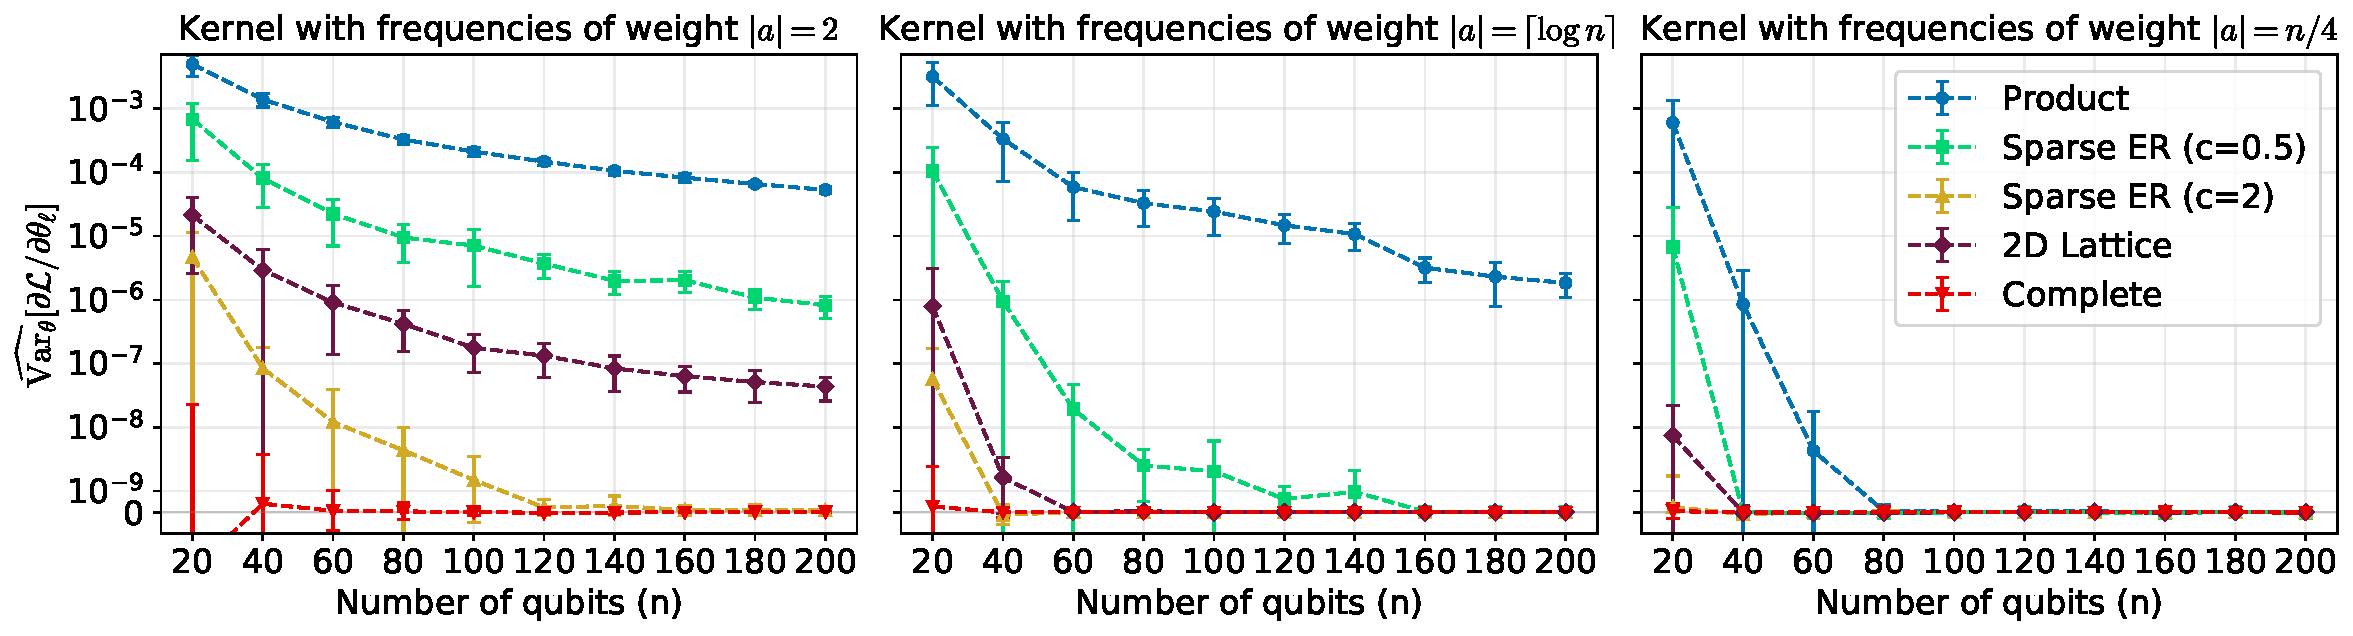
\includegraphics[width=\textwidth]
{neurips2026/bp_unbiased_uniform_mean.pdf}
%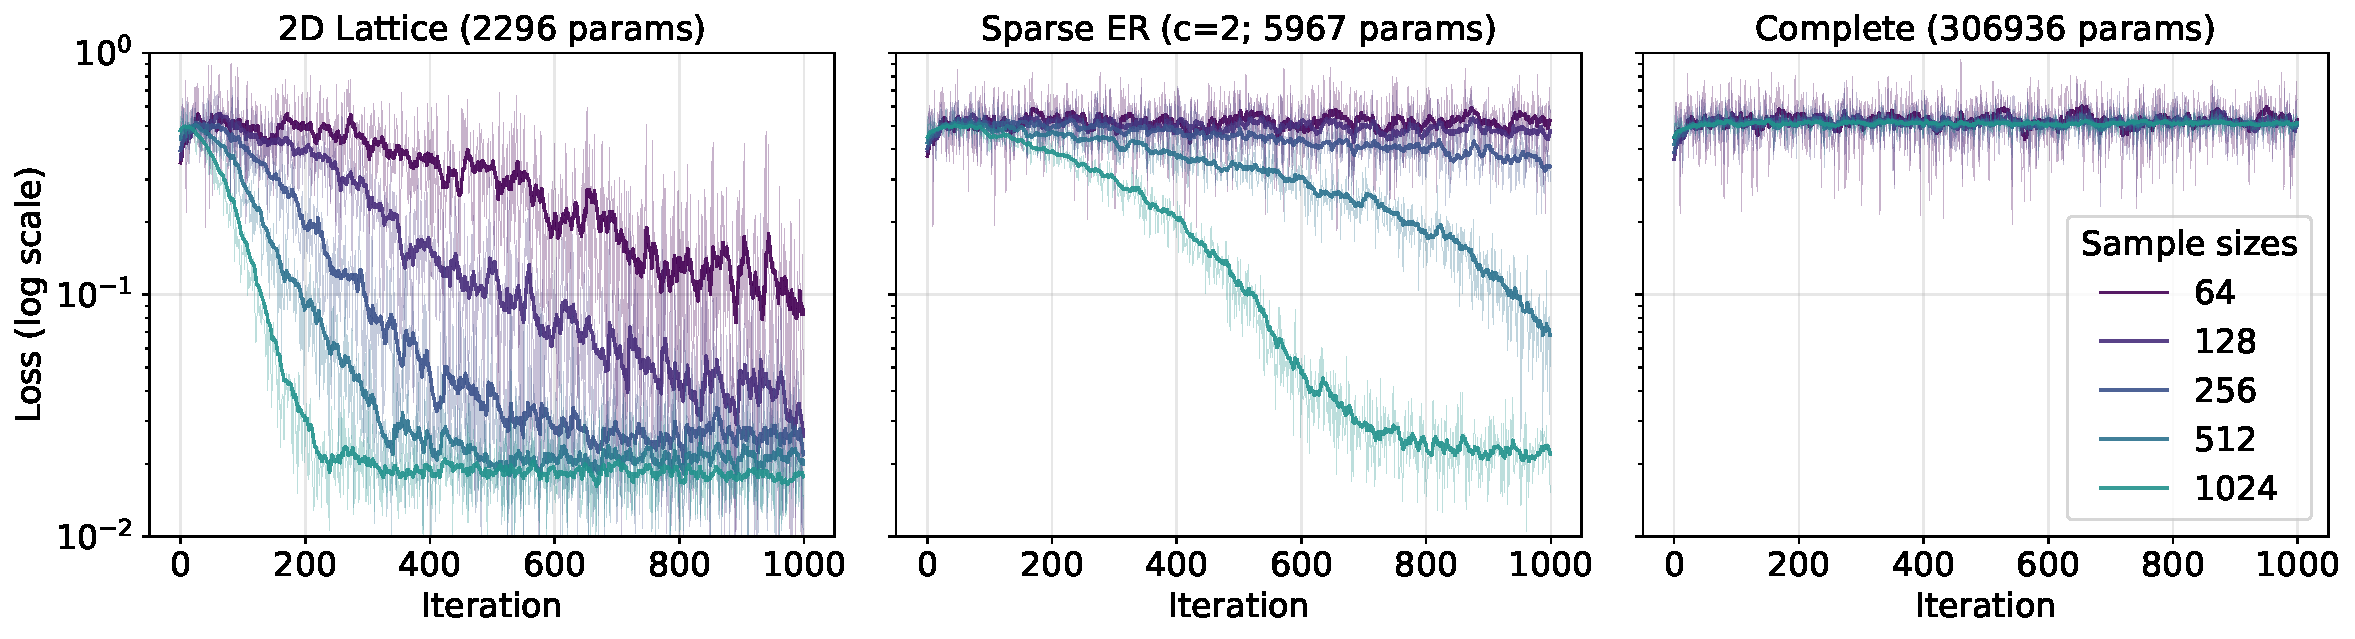
\includegraphics[width=\textwidth, trim=2mm 0mm 2mm 10mm, clip]{neurips2026/fixedOps_low_resource_training_curves.pdf}
\end{subfigure}
\begin{subfigure}{\textwidth}
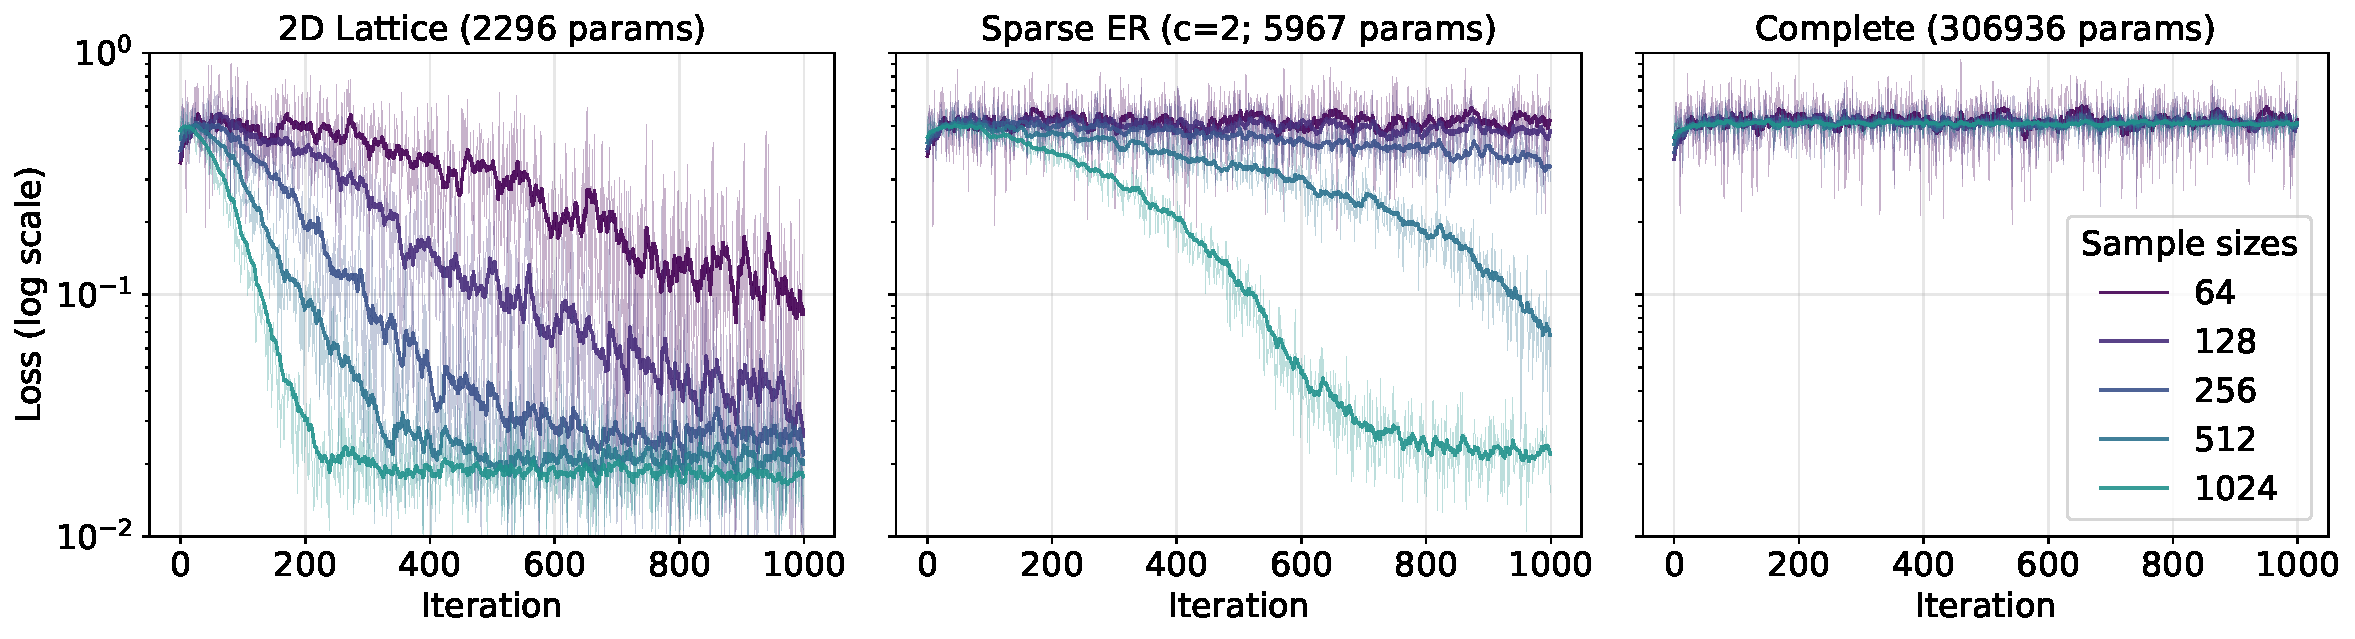
\includegraphics[width=\textwidth]
{neurips2026/fixedOps_low_resource_training_curves.pdf}
%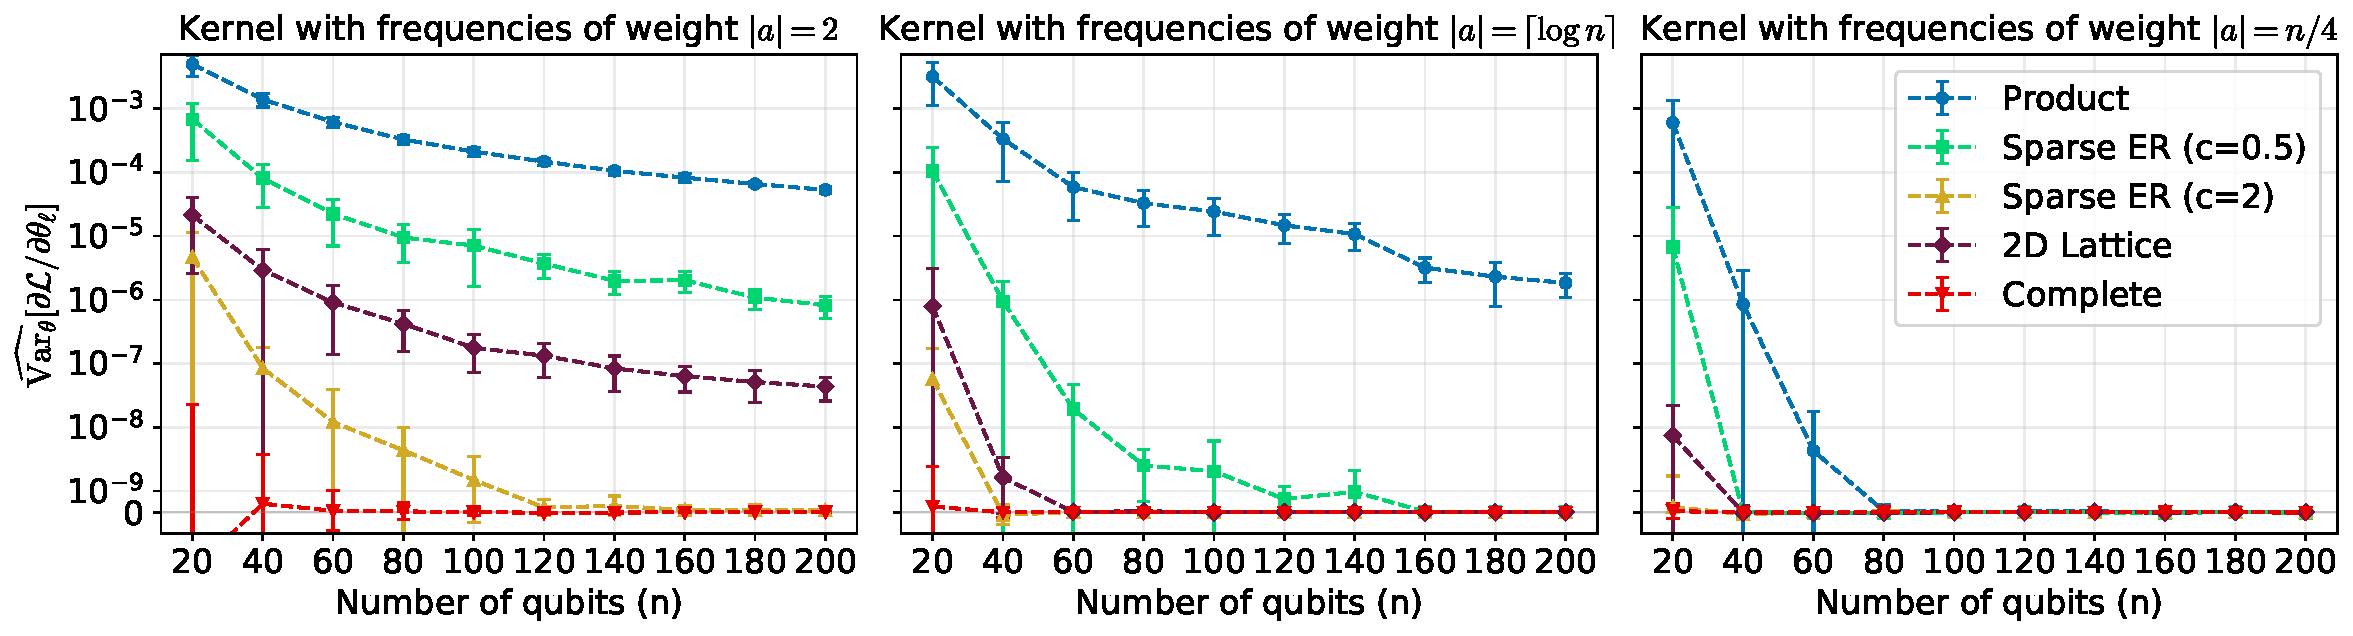
\includegraphics[width=\textwidth, trim=10mm 0mm 10mm 100mm, clip]{neurips2026/bp_unbiased_uniform_mean.pdf}
\end{subfigure}
\caption{Top: Scaling of the MMD derivative with respect to the number of qubits, measured on MNIST-inspired datasets and reporting the mean and standard deviation over $50$ repetitions. Bottom: Trajectories of the MMD training loss for learning the $784$-qubit binarized MNIST dataset, with increasing sample sizes for estimating the MMD loss.}
\label{pic:numerics}
\end{figure}
% To verify the scaling of the MMD gradient magnitudes in practice, we have created datasets of different sizes ($20,40,60,\dots,200$ bits) with marginals and correlations that approximately match the Fourier spectrum of real-world datasets MNIST. We studied all 4 architectures considered in the paper, Product, 2D Lattice, Sparse ER (with parameter $c=0.5$ or 2), and Complete graph, with different qubit numbers ranging from 20 to 200 under either uniform initialisation or Gaussian initialisation (variance is set to 1/D, D being the parameter count, consistent with our Theorem 3.13). For each setting, we estimated the magnitude of the partial derivative of the MMD loss, averaged over coordinates, with three different kernels: 
% 1. A kernel that only consists of weight-2 frequencies. 
% 2. A kernel that only consists of weight-$\log(n)$ frequencies. 
% 3. A kernel that only consists of weight-$n/4$ frequencies. 
   
% For the Sparse ER architecture, every reported data point shows the mean and std over 10 initialisation seeds and 5 random graphs. For other architectures, every reported data point shows the mean and std over 50 initialisation seeds.

% The results are shown in Figure 1 (uniform) and Figure 2 (Gaussian) below. 


% In our experiment setting, there’s a noise floor of the gradient magnitude since we use the finite sample sizes to estimate it. This is why in the figures, many curves decrease and stay flat at some value below $10^{-9}$. For the three different kernels, each architecture demonstrates either polynomial decay or exponential decay, all of which match our analysis in Examples 3.9-3.12 in our paper.
 
% To demonstrate the full training of IQP-QCBM on real world datasets, we have also performed the training on the binarized MNIST dataset (requires 784 qubits). We tested three architectures: 2D Lattice, Sparse ER, and Complete graph. The training is conducted on an RTX A6000 ADA GPU. The MMD training loss values are shown in Figure 3 below.  

% \begin{figure}[t]
% \centering

% \caption{Trajectory of MMD loss value in the training..}
% \label{pic:illustration}
% \end{figure}

% We observe that both the 2D Lattice architecture and the Sparse ER architecture show improved training stability and convergence for both Gaussian initialisation and uniform initialisation, as the sample size of estimating the MMD gradient increases. 2D Lattice shows steeper initial descent and faster convergence compared to Sparse ER in all settings, consistent with our theory (smaller critical rank in Example 3.10 and 3.11 of the paper), and this also aligns with patterns in Figure 1 and Figure 2. 

% For both architectures, for the same sample size, Gaussian initialisation provides steeper initial descent, though not a better converged value, supporting that Gaussian init mainly helps with early training, but later training dynamics and convergence are still heavily dependent on the properties of the architecture itself (e.g., gradient scaling over the entire parameter space) and the sample sizes.

% The Complete graph architecture was not trainable even at the highest sample size, consistent with the barren plateau prediction. 
% Under Gaussian initialisation, the losses fail to converge. The likely cause is, the sample size is not big enough to estimate the MMD gradient correctly.
% As shown in Figure 2, under Gaussian initialisation, the complete architecture has a signal that decays polynomially with a higher degree than the other two architectures, and hence requires more samples to estimate. It is possible that with larger sample sizes, the complete architecture will become trainable in the initial phases, under Gaussian initialisation. 

% \section{Discussion}
% \label{sec:discussion}
% We want to clarify a key difference from a related work. \citet{herbst25} claim that ``quantum models with sampling hardness rooted in anticoncentration will not be trainable.'' This claim is not in contradiction with our results, because their argument relies on pseudo-independence, a condition strictly stronger than anti-concentration: a random measure $p$ is pseudo-independent if $p(x)=Y_x / (\sum_{j=1}^{2^n} Y_j)$
% where the $Y_j$ are i.i.d. positive random variables. Pseudo-independence implies anti-concentration, but the converse is false: pseudo-independence forces all nonzero characteristic function values to vanish exponentially. By contrast, $L^2$ anti-concentration only controls the collision probability and still permits a small set of frequencies to remain polynomially visible. Our \cref{eg:sparse} illustrates precisely this distinction. 
% Finally, we emphasize that the classical sampling-hardness results for IQP circuits require anti-concentration~\citep{Bremner16,Bremner17}, not pseudo-independence.
% Related to the topic of classical non-simulability and trainability, \citet{herbst25} claim that ``quantum models with sampling hardness rooted in anticoncentration will not be trainable''. We remark that their finding is not in contradiction with our results. The reason is that their argument relies on the concept of pseudo-independence, which is a strictly stronger condition than anti-concentration. A random measure $p$ is pseudo-independent if $p(x)=Y_x / (\sum_{j=1}^{2^n} Y_j)$ where $Y_j$ are identical and independent positive random variables. In fact, pseudo-independence implies anticoncentration, but the converse is false. They claim that output distributions of IQP circuits resemble pseudo-independent distributions (which is too strong as an assumption), and they prove that for a family of pseudo-independent distributions, MMD loss value vanishes exponentially w.r.t. the qubit number $n$ and hence conclude non-trainability. Their proof relies on the fact that pseudo-independence implies that the characteristic function values for all $\vta \neq \bm{0}$ are exponentially vanishing. In contrast, $L^2$ anti-concentration alone only constrains the collision probability, but still allows a small set of frequencies to remain polynomially visible. Our \cref{eg:sparse} exactly illustrates this subtle difference. We remark again that it is the anti-concentration needed in the proof of classical sampling hardness~\cite{Bremner16, Bremner17}, not pseudo-independence. 

% Finally, we emphasize that training IQP-QCBM by minimizing $\MMD_k^2(p, q_\vttheta)$ for any choice of kernel $k$ does not imply that we can get a small total variation distance $\operatorname{TV}(p, q_\vttheta)$ since it is widely known that MMD is controlled by TV, but not vice versa. This limitation is purely classical information-theoretical, and not specific to IQP. 
% It reflects the general fact that learning an arbitrary distribution on $\{0,1\}^n$ in total variation requires exponentially many samples in the worst case, since the space has $2^n-1$ degrees of freedom. 
% What methods, like MMD, can learn efficiently are restricted families. 
\section{Conclusions and Limitations}
\label{sec:conclusion}
In this work, we studied the trainability and classical non-simulability of IQP-QCBMs. We expressed the MMD-gradient variance in terms of the IQP output's characteristic function and the kernel's spectral measure. Our first major result identifies the critical rank, which exactly determines the scaling of characteristic-function gradient variances and thereby characterizes the presence or absence of BPs. Unlike general depth-based bounds, critical ranks can be computed exactly from the generator set. We demonstrated the framework for product-state, two-dimensional lattice, sparse Erdős--Rényi, and complete-graph architectures.

% We precisely analyze whether barren plateaus occur in the MMD loss of four different IQP architectures under uniform initialization of the circuit's parameters, and demonstrate how BP can be mitigated by appropriate kernel selection.
% In particular, we focus on investigating the scaling of the characteristic function of the output distribution of IQP-QCBM and of the MMD loss function.
% We give an architecture-level characterization of trainability for IQP-QCBMs under MMD. 
% We first derive the closed-form variance expressions for the characteristic function values and the MMD and 
Our second major result concerns sparse Erd\H os-R\'enyi architectures at a suitable edge probability. Their low-weight gradients decay only polynomially, while the conditioned family is classically non-simulable in the worst case, assuming sparse average-case hardness and noncollapse of the polynomial hierarchy. Choosing a kernel concentrated on these frequencies therefore allows trainability and classical non-simulability to coexist. This contrasts with the trade-off suggested for supervised QML models, where trainability often implies classical simulability.

This does not contradict the claim of \citet{herbst25} that sampling hardness rooted in anti-concentration precludes trainability. Their argument assumes pseudo-independence, where $p(x)=Y_x/(\sum_jY_j)$ for i.i.d. positive $Y_j$. Pseudo-independence implies anti-concentration, but not conversely, and forces all nonzero characteristic functions to vanish exponentially. By contrast, $L^2$ anti-concentration controls only the collision probability and permits a small set of frequencies to remain polynomially visible, as illustrated by \cref{eg:sparse}.

Here we discuss the limitations of our work. First, our trainability analysis focuses on gradient scaling under random parameter initialization. Second, avoiding a barren plateau is a necessary, but not sufficient, condition for efficient end-to-end optimization. Third, the MMD lower bound is averaged over a target-distribution ensemble, and its implications for a particular dataset depend on the dataset's Fourier spectrum and the chosen kernel. Lastly, the classical sampling-hardness result is conditional on standard complexity-theoretic conjectures. Extending the analysis to noisy devices, broader initialization schemes, and application-specific targets are interesting future directions.

\paragraph{Acknowledgements} VD and HW were supported by the Dutch National Growth Fund (NGF), as part of the Quantum Delta NL programme.
This work was also supported by the European Union’s Horizon Europe program through the ERC CoG BeMAIQuantum (Grant No. 101124342). This research was funded by the BMW Group. 

% Lastly, we show that Gaussian initialization of the circuit's parameters leads to a polynomial decay in the variances of characteristic function values, even for high Hamming-weight frequencies, providing a potential way to broaden the set of trainable architectures in practice.

\newpage
\bibliographystyle{plainnat}
\bibliography{ref}

%%%%%%%%%%%%%%%%%%%%%%%%%%%%%%%%%%%%%%%%%%%%%%%%%%%%%%%%%%%%

\appendix

\onecolumn
\section{Proof of Theorems}
\subsection{Proof of~\cref{prop:lower}}
Consider an $n$-qubit IQP-QCBM in~\cref{def:IQP}, with generator set $S=\{\vtsj\}_{j=1}^D$, and the MMD loss $\mathcal{L}$ defined in~\cref{prop:mmd-loss}. Let $\mu_n$ be a reference measure on the parameter space that is symmetric about 0 (e.g., uniform), and let $\Lambda$ be a positive spectral probability measure on $\mathbb{F}_2^n$. Then the variance of the partial derivative of the MMD admits the decomposition
\begin{align*}
&\operatorname*{Var}_{\vttheta\sim \mu_n} \left[ \frac{\partial \mathcal{L}(\vttheta)}{\partial \theta_\ell} \right]
= 4 \operatorname*{\mathbb{E}}_{\vttheta\sim \mu_n} \left( \sum_{\vta, \vtb \in \mathbb{F}_2^n} \Lambda(\vta) \Lambda(\vtb)F(\vta, \vtb)\right)\\
&F(\vta, \vtb) = \left( C_\vttheta(\vta) C_\vttheta(\vtb) - 2C_p(\vta) C_\vttheta(\vtb) + C_p(\vta) C_p(\vtb) \right)\frac{\partial C_\vttheta(\vta)}{\partial \theta_\ell} \frac{\partial C_\vttheta(\vtb)}{\partial \theta_\ell} \nonumber
\end{align*}
\begin{proof}
We perform expansion of the term directly, using \cref{prop:mmd-loss}.
\begin{align*}
    \operatorname*{Var}_{\vttheta} \left[ \frac{\partial \mathcal{L}(\vttheta)}{\partial \theta_\ell} \right] &=    \operatorname*{Var}_{\vttheta} \left[ \frac{\partial }{\partial \theta_\ell}  \left(\sum_{\vta \in \mathbb{F}_2^n} \Lambda(\vta)\left(C_p(\vta) - C_\vttheta(\vta) \right)^2\right)\right]
\\ &= \operatorname*{Var}_{\vttheta} \left[-2 \sum_\vta \Lambda(\vta) \left(C_p(\vta) - C_\vttheta(\vta) \right) \frac{\partial C_\vttheta(\vta)}{\partial \theta_\ell} \right] \\
&= 4 \sum_{\vta, \vtb} \Lambda(\vta) \Lambda(\vtb) \operatorname*{Cov}_{\vttheta}\left(\left(C_p(\vta) - C_\vttheta(\vta)\right) \frac{\partial C_\vttheta(\vta)}{\partial \theta_\ell} , \left(C_p(\vtb) - C^\vtb_\vttheta\right) \frac{\partial C^\vtb_\vttheta}{\partial \theta_\ell} \right) \\
&= 4 \sum_{\vta, \vtb} \Lambda(\vta) \Lambda(\vtb) \bigg(\operatorname*{\mathbb{E}}_{\vttheta} \left[ (C_p(\vta) - C_\vttheta(\vta)) \frac{\partial C_\vttheta(\vta)}{\partial \theta_\ell} (C_p(\vtb) - C^\vtb_\vttheta) \frac{\partial C^\vtb_\vttheta}{\partial \theta_\ell} \right] \\
&- \operatorname*{\mathbb{E}}_{\vttheta}\left[(C_p(\vta) - C_\vttheta(\vta)) \frac{\partial C_\vttheta(\vta)}{\partial \theta_\ell} \right] \operatorname*{\mathbb{E}}_{\vttheta}\left[(C_p(\vtb) - C^\vtb_\vttheta) \frac{\partial C^\vtb_\vttheta}{\partial \theta_\ell} \right] \bigg) \\
&= 4 \operatorname*{\mathbb{E}}_{\vttheta} \left[\sum_{\vta, \vtb} \Lambda(\vta) \Lambda(\vtb)  \left( C_p(\vta) - C_\vttheta(\vta) \right) \frac{\partial C_\vttheta(\vta)}{\partial \theta_\ell} \left(C_p(\vtb) - C^\vtb_\vttheta\right) \frac{\partial C^\vtb_\vttheta}{\partial \theta_\ell} \right] \\
&= 4 \operatorname*{\mathbb{E}}_{\vttheta}\bigg[ \sum_{\vta, \vtb} \Lambda(\vta) \Lambda(\vtb) \bigg( C_p(\vta) C_p(\vtb) \frac{\partial C_\vttheta(\vta)}{\partial \theta_\ell} \frac{\partial C_\vttheta(\vtb)}{\partial \theta_\ell} - C_p(\vta) C_\vttheta(\vtb) \frac{\partial C_\vttheta(\vta)}{\partial \theta_\ell} \frac{\partial C_\vttheta(\vtb)}{\partial \theta_\ell}\\
& - C_p(\vtb) C_\vttheta(\vta) \frac{\partial C_\vttheta(\vta)}{\partial \theta_\ell} \frac{\partial C_\vttheta(\vtb)}{\partial \theta_\ell} + C_\vttheta(\vta) C_\vttheta(\vtb) \frac{\partial C_\vttheta(\vta)}{\partial \theta_\ell} \frac{\partial C_\vttheta(\vtb)}{\partial \theta_\ell}\bigg) \bigg]
\end{align*}
In the above derivation, many terms vanish. In particular, all terms of the forms $\frac{\partial C_\vttheta(\vta)}{\partial \theta_\ell}$ and $C_\vttheta(\vta)\frac{\partial C_\vttheta(\vta)}{\partial \theta_\ell}$ have zero expectation values. More specifically, these terms either vanish when $\vta \cdot\vtsl =0$ or are odd functions of $\theta_\ell$ when $\vta \cdot\vtsl =1$; their expectations vanish due to the symmetry of $\mu_n$.
\end{proof}
Consider averaging this quantity over an unbiased ensemble of target distributions $\mathcal P$. Specifically, we assume that, $\forall\vta, \vtb \in \mathbb{F}_2^n \setminus \{\bm{0}\},\operatorname*{\mathbb {E}}_{p\sim\mathcal {P}}[C_p(\vta)]=0$, and $\operatorname*{\mathbb {E}}_{p\sim\mathcal {P}}\!\left[C_p(\vta)C_p(\vtb)\right]=\delta_{\vta,\vtb}\,\sigma^2(\vta)$, where $\sigma^2(\vta) = \operatorname*{\mathbb {E}}_{p \sim \mathcal{P}}\left[C_p(\vta)^2\right]$. Under this ensemble average, we obtain the lower bound:
\begin{equation*}
\operatorname*{\mathbb{E}}_{p\sim\mathcal{P}} \left[\operatorname*{Var}_{\vttheta\sim\mu_n}  
\left[\frac{\partial \mathcal{L}(\vttheta)}{\partial \theta_\ell} \right]\right] \geq
4 \sum_{\vta\in \mathbb{F}_2^n} \Lambda^2(\vta)\sigma^2(\vta)\operatorname*{Var}_{\vttheta\sim\mu_n} \left[ \frac{\partial C_\vttheta(\vta)}{\partial \theta_\ell} \right].
\end{equation*}
\begin{proof}
Continuing from the proof above, we first identify the four-copy terms as square terms, i.e., 
\begin{equation*}
    \operatorname*{\mathbb{E}}_{\vttheta} \left[ \sum_{\vta, \vtb} \Lambda(\vta) \Lambda(\vtb) C_\vttheta(\vta) C_\vttheta(\vtb) \frac{\partial C_\vttheta(\vta)}{\partial \theta_\ell} \frac{\partial C_\vttheta(\vtb)}{\partial \theta_\ell}\right] =\operatorname*{\mathbb{E}}_{\vttheta}\left[ \left(\sum_{\vta \in \mathbb{F}_2^n} \Lambda(\vta) C_\vttheta(\vta) \frac{\partial C_\vttheta(\vta)}{\partial \theta_\ell}\right)^2\right]
\end{equation*}
which we can safely drop in the lower bound as non-negative terms. 
%As explained in the main text, a finer analysis shows that these terms sum to an exponentially small positive quantity, which we neglect.

Then we can apply the ensemble average. All the three-copy terms $C_p(\vta) C_\vttheta(\vtb) \frac{\partial C_\vttheta(\vta)}{\partial \theta_\ell} \frac{\partial C_\vttheta(\vtb)}{\partial \theta_\ell}$ vanish. Due to the uncorrelatedness between $C_p(\vta)$ and $C_p(\vtb)$, all the off-diagonal two copy terms $C_p(\vta) C_p(\vtb) \frac{\partial C_\vttheta(\vta)}{\partial \theta_\ell} \frac{\partial C_\vttheta(\vtb)}{\partial \theta_\ell}$ also vanish. Finally, we obtain the desired non-trivial lower bound for an average-case problem.
\begin{align*}
 \operatorname*{\mathbb{E}}_p\left[\operatorname*{Var}_{\vttheta} \left[ \frac{\partial \mathcal{L}(\vttheta)}{\partial \theta_\ell} \right]\right] &\geq 4 \operatorname*{\mathbb{E}}_{\vttheta}  \left[ \sum_{\vta \in \mathbb{F}_2^n} \Lambda(\vta)^2 (C_p(\vta))^2 \left(\frac{\partial C_\vttheta(\vta)}{\partial \theta_\ell}\right)^2 \right] \\
 &= 4 \sum_a\Lambda(\vta)^2\sigma_\vta^2\operatorname*{Var}_{\vttheta} \left[ \frac{\partial C_\vttheta(\vta)}{\partial \theta_\ell} \right] 
\end{align*}
\end{proof}

\subsection{Proof of \cref{prop:upper}}
Under the same conditions as in~\cref{prop:lower}, the variance of the partial derivative of the MMD satisfies
\begin{equation*}
    \operatorname*{Var}_{\vttheta \sim\mu_n} \left[ \frac{\partial \mathcal{L}(\vttheta)}{\partial \theta_\ell} \right] \leq 16 \sum_{\vta\in \mathbb{F}_2^n} \Lambda(\vta)\left[  \operatorname*{Var}_{\vttheta\sim\mu_n} \left[ \frac{\partial C_\vttheta(\vta)}{\partial \theta_\ell} \right]\right]
\end{equation*}
\begin{proof}
\begin{align*}
\operatorname*{Var}_{\vttheta} \left[ \frac{\partial \mathcal{L}(\vttheta)}{\partial \theta_\ell} \right] &\leq \operatorname*{\mathbb{E}}_{\vttheta} \left[ \left(\frac{\partial \mathcal{L}(\vttheta)}{\partial \theta_\ell} \right)^2 \right] \\
&= 4\operatorname*{\mathbb{E}}_{\vttheta} \left[  \operatorname*{\mathbb{E}}_{\vta}\left[\left( C_p(\vta) - C_\vttheta(\vta) \right) \frac{\partial C_\vttheta(\vta)}{\partial \theta_\ell} \right]^2  \right]\\
&\leq 4\operatorname*{\mathbb{E}}_{\vttheta} \left[  \operatorname*{\mathbb{E}}_{\vta}\left[\left( C_p(\vta) - C_\vttheta(\vta) \right)^2 \right] \operatorname*{\mathbb{E}}_{\vta}\left[\left(\frac{\partial C_\vttheta(\vta)}{\partial \theta_\ell} \right)^2\right]\right]\\
&\leq 4\operatorname*{\mathbb{E}}_{\vttheta} \left[  4 \operatorname*{\mathbb{E}}_{\vta}\left[\left(\frac{\partial C_\vttheta(\vta)}{\partial \theta_\ell} \right)^2\right]\right]\\
&= 16 \sum_\vta \Lambda(\vta)\left[  \operatorname*{Var}_{\vttheta} \left[ \frac{\partial C_\vttheta(\vta)}{\partial \theta_\ell} \right]\right]
\end{align*}
In the derivation above, we first used the Cauchy--Schwarz inequality and then the bound that, for a fixed $\vta$, $(C_p(\vta) - C_\vttheta(\vta))^2 \leq 4$. Lastly, we exchanged the order of expectations over $\vta$ and $\vttheta$ and used the fact that $\operatorname*{\mathbb{E}}_{\vttheta}\left[\partial C_\vttheta(\vta) / \partial \theta_\ell\right] = 0$.
\end{proof}


\subsection{Proof of \cref{thm:uniform}}
Before proving \cref{thm:uniform}, we will first prove a more general result applying to a broader family of reference measures that are symmetric about $0$, from which \cref{thm:uniform} follows as a special case.

We wish to show that: Let $\theta_1,\dots,\theta_D$ be i.i.d.\ with a common distribution that is symmetric about $0$. For a fixed Fourier frequency $\vta \in \mathbb{F}_2^n$, define $S^{\vta} := \{ \vtsj \big| \vta \cdot \vtsj = 1 \}$, $
m^\vta := \abs{S^{\vta}}$. Let $
\Xi^\vta:= \{J\subseteq S^\vta:\ \sum_{j\in J}\vtsj=\mathbf 0 \}.$ Then, 
%%%%%%%%%
\begin{equation*}
\operatorname*{\mathbb{E}}_\vttheta\big[C_\vttheta(\vta)\big] = \kappa^{m^\vta}, \qquad
\operatorname*{\mathbb{E}}_\vttheta\big[C_\vttheta(\vta)^2\big] = \sum_{J\in \Xi^\vta} \mu^{|J|} \nu^{m^\vta-|J|},
\end{equation*}
and hence
\begin{equation*}
     \operatorname*{Var}_\vttheta \left[ C_\vttheta(\vta) \right] = 
\left(\sum_{J\in \Xi^\vta} \mu^{|J|} \nu^{m^\vta-|J|}\right) - \kappa^{2m^\vta},
\end{equation*}
%%%%%%%%%
where $\mu=\operatorname*{\mathbb{E}}[\sin^2(2\theta_1)]$, $\nu=\operatorname*{\mathbb{E}}[\cos^2(2\theta_1)]$, $\kappa=\operatorname*{\mathbb{E}}[\cos(2\theta_1)]$. Fix $\ell\in[D]$. If $\vtsl \notin S^\vta$, then $ \frac{\partial C_\vttheta(\vta)}{\partial \theta_\ell}=0$. If $\vtsl \in S^\vta$, then, 
%%%%%%%%%
\begin{align*}
\operatorname*{Var}_\vttheta \left[ \frac{\partial C_\vttheta(\vta)}{\partial \theta_\ell} \right]
&= 4\sum_{J\in \Xi^\vta}
\Bigl[
\bm{1}\{\ell\in J\}\,\mu^{|J|-1}\nu^{m^\vta-|J|+1} \notag
\\&+
\bm{1}\{\ell\notin J\}\,\mu^{|J|+1}\,\nu^{m^\vta-|J|-1}\Bigr].
\label{eq:symmetric-variance}
\end{align*}
%%%%%%%%%

\begin{proof}
Fix $\vta\in\mathbb{F}_2^n$ and abbreviate $S:=S^\vta$, $m:=m^\vta$. If $m=0$, then $X^\vta$ commutes with $U_\vttheta$, so $C_\vttheta(\vta)\equiv 1$; this agrees with all formulas above, since then $\Xi^\vta=\{\emptyset\}$ and $\kappa^{0}=1$. Assume $m\geq 1$ from now on. Start from the expression $C_\vttheta(\vta)=\bra{+} U_\vttheta^\dagger X^{\vta}U_\vttheta\ket{+}
$. By recursively swapping the gates in $U_\vttheta$ with the observable $X^{\vta}$ and applying the commutation or anticommutation rule, one can derive the following:
\begin{align*}
C_\vttheta(\vta)
&= \bra{+}^{\otimes n} \prod_{\vtsj\in S^\vta} \exp(-2i\theta_jZ^\vtsj) \ket{+}^{\otimes n} \\
&= \bra{+}^{\otimes n} \prod_{\vtsj\in S^\vta} (\cos(2\theta_j)I - i \sin(2\theta_j)Z^\vtsj) \ket{+}^{\otimes n}  \\
&= \sum_{J\in\Xi^\vta} R_J(\vttheta), \qquad R_J(\vttheta)=\eta_J 
\Bigl(\prod_{j\in J} \sin(2\theta_j)\Bigr)\Bigl(\prod_{j\in S\setminus J}\cos(2\theta_j)\Bigr),
\end{align*}
where $\eta_J \in \{-1,1\}$. The equation is a reformulation of equation 27 of \cite{recioarmengol25}. Note that $\forall J \in \Xi^\vta, \abs{J} = 0 \, (\text{mod 2})$, so no imaginary number $i$ appears. Also note that $\sin(\cdot)$ is an odd function, whose expectation vanishes for any symmetric distribution. We will use this property many times.

First, we derive the variance of the characteristic function values, $\operatorname*{Var}_\vttheta \left[ C_\vttheta(\vta) \right] = \operatorname*{\mathbb{E}}_\vttheta \left[ (C_\vttheta(\vta))^2\right] - \left(\operatorname*{\mathbb{E}}_\vttheta \left[ C_\vttheta(\vta) \right]\right)^2$. Regarding $\operatorname*{\mathbb{E}}_\vttheta \left[ C_\vttheta(\vta) \right]$, except for the empty set $J = \emptyset$ (for which $\eta_\emptyset=1$), all the other terms in the summation contain $\sin(2\theta_j)$ for some $j$ and hence vanish in expectation by independence, so $\operatorname*{\mathbb{E}}_\vttheta[C_\vttheta(\vta)]=\kappa^{m}$. Regarding $\operatorname*{\mathbb{E}}_\vttheta \left[ (C_\vttheta(\vta))^2\right]$, for the same reason, $\forall J \neq K$,  $\operatorname*{\mathbb{E}}_{\vttheta}[R_J(\vttheta)R_K(\vttheta)] = 0$, since $R_JR_K$ contains a single factor $\sin(2\theta_j)$ for every $j\in J\triangle K\neq\emptyset$. Putting the remaining terms together gives
\begin{equation*}
     \operatorname*{\mathbb{E}}_\vttheta \left[ C_\vttheta(\vta)^2 \right] = \sum_{J \in \Xi^\vta} \operatorname*{\mathbb{E}}_\vttheta[R_J(\vttheta)^2] = \sum_{J \in \Xi^\vta} \mu^{\abs{J}} \nu^{m-\abs{J}},
\end{equation*}
and subtracting $\operatorname*{\mathbb{E}}_\vttheta[C_\vttheta(\vta)]^2=\kappa^{2m}$ gives the variance.
Then, we derive the variance of the partial derivatives. We differentiate the terms $R_J(\vttheta)$ with respect to $\theta_\ell$. If $\vtsl \notin S^\vta$, then $\comm{Z^{\vtsl}}{X^\vta}=0$, so $C_\vttheta(\vta)$ is independent of $\theta_\ell$, giving $\frac{\partial C_\vttheta(\vta)}{\partial \theta_\ell}=0$. Now, if $\vtsl \in S^\vta$,

\begin{equation*}
\frac{\partial C_\vttheta(\vta)}{\partial\theta_\ell}
=
\sum_{J\in\Xi^\vta} T_J(\vttheta),
\end{equation*}
where
\begin{equation*}
T_J(\vttheta)
=
\begin{cases}
2 \eta_J\prod_{j\in J\setminus\{\ell\}}\sin(2\theta_j)\prod_{j\in (S\setminus J) \cup \{\ell\}}\cos(2\theta_j), & \ell\in J,\\
-2 \eta_J \prod_{j\in J\cup \{\ell \}}\sin(2\theta_j)\prod_{j\in (S\setminus J)\setminus\{\ell\}}\cos(2\theta_j), & \ell\notin J.
\end{cases}
\label{eq:TJ_def}
\end{equation*}
For the same reason as before, $\operatorname*{\mathbb{E}}_{\vttheta}[T_J(\vttheta)T_K(\vttheta)] = 0 $ and  $\operatorname*{\mathbb{E}}_{\vttheta} \left[ \frac{\partial C_\vttheta(\vta)}{\partial\theta_\ell}\right] = 0.$
Therefore,
\begin{equation*}
\operatorname*{Var}_{\vttheta}\left[\frac{\partial C_\vttheta(\vta)}{\partial\theta_\ell}\right]
=
\operatorname*{\mathbb{E}}_{\vttheta}\left[\left(\frac{\partial C_\vttheta(\vta)}{\partial\theta_\ell}\right)^2\right]
=
\sum_{J\in \Xi^\vta}\operatorname*{\mathbb{E}}_{\vttheta}[T_J(\vttheta)^2],
\label{eq:symmetric-derivative-variance}
\end{equation*}
Finally, computing $\operatorname*{\mathbb{E}}_\vttheta[T_J(\vttheta)^2]$ from the two cases of $T_J$ above gives the desired result.
\end{proof}

Now we are ready to prove \cref{thm:uniform}. Consider an $n$-qubit IQP-QCBM in~\cref{def:IQP} with the generator set $S=\{\vtsj\}_{j=1}^D$, and let the reference measure on the parameter space be uniform, namely $\mu_n = \mathcal{U}([0,2\pi)^D)$. For a frequency $\vta \in \mathbb{F}_2^n$, define $S^{\vta} \coloneqq \{ \vtsj\in S \mid \vta \cdot \vtsj = 1 \}$ and the critical rank $r^\vta \coloneqq \dim \operatorname{span}_{\mathbb{F}_2}( S^{\vta})$ (so $r^\vta=0$ if $S^\vta=\emptyset$, in particular $r^{\mathbf 0}=0$). Then
\begin{equation*}
\operatorname*{\mathbb{E}}_{\vttheta\sim\mu_n}\big[C_\vttheta(\vta)^2\big] = 2^{-r^\vta},
\end{equation*}
and if $S^\vta\neq\emptyset$, then $\operatorname*{\mathbb{E}}_{\vttheta}[C_\vttheta(\vta)]=0$, hence $\operatorname*{Var}_{\vttheta\sim\mu_n}[C_\vttheta(\vta)] = 2^{-r^\vta}$. (If $S^\vta=\emptyset$, then $C_\vttheta(\vta)\equiv 1$.) For $\ell \in [D]$, if $\vtsl \notin S^\vta$, then $ \frac{\partial C_\vttheta(\vta)}{\partial \theta_\ell}=0$. If $\vtsl \in S^\vta$, then
\begin{equation*}
\operatorname*{Var}_{\vttheta\sim\mu_n} \left[ \frac{\partial C_\vttheta(\vta)}{\partial \theta_\ell} \right] = 2^{\,2-r^\vta}. \end{equation*}
\begin{proof}
Using the same notations as in the previous proof, in the case of uniform distribution, $\mu = \nu = 1/2$ and $\kappa = 0$. Plugging in these values gives, \begin{equation*}
    \operatorname*{\mathbb{E}}_\vttheta \left[ C_\vttheta(\vta)^2 \right] = 2^{-m^\vta} \abs{\Xi^\vta} , \qquad \operatorname*{Var}_{\vttheta}\left[\frac{\partial C_\vttheta(\vta)}{\partial\theta_\ell}\right]
= 2^{2-m^\vta} \abs{\Xi^\vta} .
\end{equation*}
Note that $\Xi^\vta$ is isomorphic to the set $\{\vtx \in \mathbb{F}_2^{m^\vta} | H \vtx = \bm{0}\}$, where $H$ is the matrix whose columns are the elements of $S^\vta$. In other words, $\Xi^\vta$ is the kernel of $H$ and hence $\abs{\Xi^\vta} = 2^{m^\vta-r^\vta}$ by the rank-nullity theorem (this also holds for $m^\vta=0$, where $\Xi^\vta=\{\emptyset\}$). This gives $\operatorname*{\mathbb{E}}_\vttheta[C_\vttheta(\vta)^2]=2^{-r^\vta}$ and the derivative formula. Finally, $\operatorname*{\mathbb{E}}_\vttheta[C_\vttheta(\vta)]=\kappa^{m^\vta}=0$ whenever $m^\vta\geq1$, i.e.\ $S^\vta\neq\emptyset$, in which case $\operatorname*{Var}_\vttheta[C_\vttheta(\vta)]=\operatorname*{\mathbb{E}}_\vttheta[C_\vttheta(\vta)^2]=2^{-r^\vta}$. This completes the proof.
\end{proof}
 

% \subsection{Proof of \cref{thm:poly_lb_gaussian_mmd}}
% Consider an $n$-qubit IQP-QCBM $U_\vttheta$ with generators $\{\vtsj\}$ of arbitrary architecture. Consider that the parameters $\vttheta$ are i.i.d. and Gaussian $\theta_j \sim\mathcal{N}(0,\gamma^2)$, with variance $\gamma^2 = c/D$ for arbitrary constant $c$. Fix $1\leq l \leq D$. For any frequency $\vta \in \mathbb{F}_2^n$, if $\in S^\vta$, then 
% \begin{equation}
% \operatorname*{Var}_{\vttheta} \left[ \frac{\partial C_\vttheta(\vta)}{\partial \theta_\ell} \right] = \Omega\left(\mathrm{poly}(n^{-1})\right).
% \end{equation} 
% If $\vtsl \notin S^\vta$, then $\frac{\partial C_\vttheta(\vta)}{\partial \theta_\ell}=0$.
% \begin{proof}
% We assume that $\vta \in \vtsl$ and continue from \cref{eq: symmetric variance} of \cref{thm: single symmetric},
% \begin{equation}
% \operatorname*{Var}_{\vttheta}\!\left(\frac{\partial C_\vttheta(\vta)}{\partial\theta_\ell}\right)
% =
% 4\sum_{J\in \Omega^\vta}
% \left[
% \bm{1}\{\ell\in J\}\,\mu^{|J|-1}\nu^{m^\vta-|J|+1}
% +
% \bm{1}\{\ell\notin J\}\,\mu^{|J|+1}\,\nu^{m^\vta-|J|-1}
% \right],
% \label{eq:single_var_exact_c}
% \end{equation}
% We identify \begin{equation}
%     \mu:=\operatorname*{\mathbb{E}}_{\theta\sim\mathcal N(0,\gamma^2)}[\sin^2(2\theta)]
% =\frac{1-e^{-8\gamma^2}}{2},
% \qquad
% \nu:=\operatorname*{\mathbb{E}}_{\theta\sim\mathcal N(0,\gamma^2)}[\cos^2(2\theta)]
% =\frac{1+e^{-8\gamma^2}}{2}
% \end{equation} 
% Note that every term in the summation is nonnegative. For the proof it suffices to keep the term $J= \emptyset$ and drop other terms, which gives
% \begin{align}
% \operatorname*{Var}_{\vttheta}\!\left(\frac{\partial C_\vttheta(\vta)}{\partial\theta_\ell}\right) & \geq 
% 4\mu\,\nu^{m^\vta-1} \\
% & \geq  4\mu\,\nu^{D-1} 
% \label{eq:single_var_lb_c}
% \end{align}
% By Taylor expansion, we can derive that $\mu = 4c/D + o(1/D)$ and $\nu^{D-1} = e^{-4c} + o(1)$. Therefore, $4\mu \nu^{D-1} =\Theta(1/D)$, which completes the proof.
% \end{proof}

\subsection{Proof of \cref{lem:parseval}}
Let $Q=\{q_\vttheta\}_\vttheta$ be the ensemble of output distributions of an
$n$-qubit IQP-QCBM with $\vttheta\sim\mathcal U([0,2\pi)^D)$, and let
$\mathcal Z \coloneqq \sum_{\vta\in\mathbb{F}_2^n} 2^{-r^\vta}$, with $r^{\mathbf 0}=0$.
Then the expected collision probability is exactly
\begin{equation}\label{eq:collision-identity}
\operatorname*{\mathbb{E}}_{\vttheta}\Big[\sum_{x\in\{0,1\}^n} q_\vttheta(x)^2\Big]
= \frac{\mathcal Z}{2^n}.
\end{equation}
Consequently, $Q$ is $L^2$ anti-concentrated with constant $b$ if and only if
$\mathcal Z\le b$. 

\begin{proof}
For fixed $\vttheta$, $C_\vttheta(\vta)=\sum_{x}(-1)^{\vta\cdot x}q_\vttheta(x)$ is the
(unnormalised) Walsh--Hadamard transform of $q_\vttheta$. Parseval's identity gives
$\sum_{\vta\in\mathbb{F}_2^n} C_\vttheta(\vta)^2 = 2^n\sum_x q_\vttheta(x)^2$ for every
$\vttheta$. Taking expectations over $\vttheta$ (both sums are finite) and using
$\operatorname*{\mathbb{E}}_\vttheta[C_\vttheta(\vta)^2]=2^{-r^\vta}$ for all $\vta$
(\cref{thm:uniform}) yields \cref{eq:collision-identity}. The equivalence follows by
comparing \cref{eq:collision-identity} with \cref{def:anti-concentration}.
\end{proof}

\subsection{Proof of \cref{thm:erm-sharp}}
\label{app:er-merged}
Let $c>0$ and $p=c\ln n/n$. Let $G\sim G(n,p)$ be an Erd\H{o}s--R\'enyi graph instance. The expected quantity $\mathbb{E}_G[\mathcal Z(G)]$ can be bounded by:
\begin{equation}
2\sum_{k=0}^{K}\frac{\big(T_n(1-o(1))\big)^k}{k!}-\mathcal O\big(n^{2K}2^{-n}\big)\ \le\ \operatorname*{\mathbb{E}}_G\big[\mathcal Z(G)\big]\ \le\ 2\exp\big(T_n(1+o(1))\big)+e^{-\Omega(n/\ln^3n)}
\end{equation}
for every fixed $K\in\mathbb N$, where $T_n=n2^{-n}(2-p)^{n-1}$. In particular, a threshold occurs at $c=2$:
\begin{equation}
    \begin{cases}
    c<2 & \lim\limits_{n\to \infty} T_n = \infty, \lim\limits_{n\to \infty}\mathbb{E}_G[\mathcal Z(G)] = \infty \\
    c=2 & \lim\limits_{n\to \infty}T_n = \frac{1}{2}, \lim\limits_{n\to \infty}\mathbb{E}_G[\mathcal Z(G)] = 2\sqrt{e}\\
    c>2 & \lim\limits_{n\to \infty}T_n = 0, \lim\limits_{n\to \infty}\mathbb{E}_G[\mathcal Z(G)] = 2 
\end{cases}
\end{equation}

\begin{proof}
Recall that by \cref{lem:parseval}, the ensemble of the output distributions of a fixed graph $G$ is anti-concentrated iff $\mathcal Z(G)\in\mathcal O(1)$, where we write $\mathcal Z(G):=\sum_{\vta\in\mathbb F_2^n}2^{-r^\vta(G)}$. 

For a fixed Fourier frequency $\vta \in \mathbb{F}_2^n$, let $A$ be the support of the observable $X^\vta$, and write $\abs{A}=k$. We denote its open neighborhood by $B$. As detailed in \cref{eg:sparse}, $\abs{B} \sim \mathrm{Binomial}(n-k,\,q)$, where we write $q = 1-\lambda^{k}$ and $\lambda=1-p$. Note that $r^\vta = k + \abs{B}$. Evaluating the probability generating function $\mathbb E[x^{|B|}]=(1-q+qx)^{n-k}$ at $x=\frac12$ gives $\mathbb{E}_G[2^{-r^\vta}]=2^{-k}(1-\frac q2)^{n-k}=2^{-k}\big(\frac{1+\lambda^k}{2}\big)^{n-k}$. Summing over all frequencies and binomially expanding $(1+\lambda^k)^{n-k}$ gives
\begin{align}\label{eq:erm-exact}
\operatorname*{\mathbb{E}}_G\big[\mathcal Z(G)\big]
&= \sum_{\vta\in\mathbb F_2^n} \mathbb{E}_G[2^{-r^\vta}] \\
&=\sum_{k=0}^n \binom nk2^{-n} \big(1+\lambda^k\big)^{n-k} \label{eq:t_k sum}\\
&= \sum_{k=0}^n \binom nk2^{-n} \sum_{j=0}^{n-k} \binom {n-k}j \lambda^{jk} \\
&=\sum_{j+k\le n}F(j,k), \label{eq:s_k sum}
\end{align}
where $F(j,k):=\frac{2^{-n}\,n!\,\lambda^{kj}}{k!\,j!\,(n-k-j)!}=F(k,j)$ is symmetric. 

For convenience, let $t_k=\binom nk2^{-k}\big(\frac{1+\lambda^k}{2}\big)^{n-k}$ such that \eqref{eq:t_k sum} writes $\operatorname*{\mathbb{E}}_G\big[\mathcal Z(G)\big] = \sum\limits_{k=0}^n t_k$. Let $s_k:=\sum_{j\ge k}F(k,j)$ and note that $s_0=2^{-n}\sum\limits_{j=0}^n\binom nj=1$. Then following from \eqref{eq:s_k sum}, 
\begin{equation}\label{eq:erm-upper}
\operatorname*{\mathbb{E}}_G\big[\mathcal Z(G)\big]=2\sum_{k=0}^{n} s_k-\sum_{k=0}^{n}F(k,k)\le2+2\sum_{k=1}^{n}s_k .
\end{equation}
Now we prove the upper bound part of \cref{thm:erm-sharp}. Let $k_1:=\lfloor n/\ln^3n\rfloor$ and $k_2:=\lfloor n/\sqrt{\ln n}\rfloor$. We will split the series $\sum\limits_{k=1}^{n} s_k$ into three parts and bound each part separately. 

\medskip
\noindent
For $1\leq k \leq k_1$, it is simpler to bound $t_k$ and then use $s_k\leq t_k$. Using the standard inequalities $\lambda^k=(1-p)^k\le e^{-kp}$, $1-e^{-x}\ge\frac{x}{1+x}$ for $x\ge0$, and $1-x\le e^{-x}$, we have that
\begin{equation}
\frac{1+\lambda^k}{2}\ = 1- \frac{1-\lambda^k}{2} \le 1- \frac{1-e^{-kp}}{2} \le\ 1-\frac{kp}{2(1+kp)}\ \le\ \exp\Big(-\frac{kp}{2(1+kp)}\Big),
\end{equation}
Raising this to the power $n-k$ and using $(n-k)p=c\ln n\,(1-\frac kn)$ gives
\begin{equation}
\Big(\frac{1+\lambda^k}{2}\Big)^{n-k} \leq
\exp\Big(-k\cdot\frac c2\cdot\frac{1-k/n}{1+kp}\,\ln n\Big)=n^{-k\alpha_k}, \quad \alpha_k=\frac c2\cdot\frac{1-k/n}{1+kp}.
\end{equation}

Then, using that $\binom nk\le\frac{n^k}{k!}$ gives
\begin{equation}\label{eq:erm-boundA}
s_k\ \le\ t_k\ \le\ \frac{n^k}{k!}\,2^{-k}\,n^{-k\alpha_k}=\frac1{k!}\Big(\frac12\,n^{1-\alpha_k}\Big)^k .
\end{equation}

We have that $k/n\le1/\ln^3n$ and $kp\le c/\ln^2n$. Using $\frac1{1+x}\ge1-x$ for $x>0$,
\begin{equation}
\alpha_k\ \ge\ \frac c2\Big(1-\frac kn\Big)(1-kp)\ \ge\ \frac c2\Big(1-\frac kn-kp\Big)\ \ge\ \frac c2-\varepsilon_n,
\qquad \varepsilon_n=\frac c2\Big(\frac1{\ln^3n}+\frac c{\ln^2n}\Big).
\end{equation}
Then, on one hand
\begin{equation}
n^{1-\alpha_k}\le n^{1-c/2}\,e^{\varepsilon_n\ln n}=n^{1-c/2}\big(1+o(1)\big).
\label{eq:erm-Sk}
\end{equation}

On the other hand, using $np^2\to0$, $T_n=t_1$ satisfies
\begin{align}
T_n&=n2^{-n}(2-p)^{n-1} \\
&=\frac{n}{2-p}\Bigl(1-\frac{p}{2}\Bigr)^n \\
&=\frac{n}{2-p} \exp\left(-\frac{np}{2} + \mathcal{O}(np^2)\right) \\
&= \Big(\frac{1}{2} + o(1)\Big)n^{1-c/2}
\label{eq:erm-Tn}
\end{align}
% which tends to $0$, $\frac12$ or $\infty$ depending on whether $c>2$, $c=2$ or $c<2$. It remains to show that, up to small errors, $\operatorname*{\mathbb{E}}_G\big[\mathcal Z(G)\big]$ behaves like $2e^{T_n}$. 
Inserting \eqref{eq:erm-Sk} and \eqref{eq:erm-Tn} into \eqref{eq:erm-boundA} gives, for large $n$,
\begin{equation}
\sum_{k=1}^{k_1}s_k\ \le\ \sum_{k=1}^{k_1}\frac{\big(T_n(1+o(1))\big)^k}{k!}\leq\exp\big(T_n(1+o(1))\big)-1. \label{eq:region-1}
\end{equation}

\medskip
\noindent
For $k_1 < k \leq k_2$, \eqref{eq:erm-boundA} still holds, and we will bound $t_k$ with a different method. We have that $k\le n/\sqrt{\ln n}$, so $1-\frac kn\ge1-\frac1{\sqrt{\ln n}}$, and $1+kp\le1+c\sqrt{\ln n}$. Hence, for large $n$,
\begin{equation}
\alpha_k\ \ge\ \frac c2\cdot\frac{1-1/\sqrt{\ln n}}{1+c\sqrt{\ln n}}=\frac{1+o(1)}{2\sqrt{\ln n}}\ \ge\ \frac1{3\sqrt{\ln n}} \implies n^{-\alpha_k}\le e^{-\sqrt{\ln n}/3}.
\end{equation} Moreover, using that $n/k<\ln^3n$ and $k!\ge(k/e)^k$, for large $n$, \eqref{eq:erm-boundA} leads to
\begin{equation}
s_k \leq \Big(\frac e2 \frac nk n^{-\alpha_k}\Big)^k \leq \Big(\frac e2 \ln^3n e^{-\sqrt{\ln n}/3}\Big)^k \leq 2^{-k}
\end{equation}
The last inequality holds for large $n$ because $\frac e2\ln^3n\,e^{-\sqrt{\ln n}/3}\to0$. Hence, for large $n$, \begin{equation}
    \sum_{k=k_1+1}^{k_2}s_k\le2^{-k_1} \label{eq:region-2}
\end{equation}

\medskip
\noindent
For $k>k_2$, we bound $s_k$ directly. Note that
\begin{equation}
s_k=\binom nk2^{-n}\sum_{j=k}^{n-k}\binom{n-k}{j}\lambda^{kj}.
\end{equation}
For $j\geq k$ and $\lambda\leq 1$, we have that $\lambda^{kj}\leq\lambda^{k^2}$. Moreover, $\sum\limits_{j=k}^{n-k}\binom{n-k}{j}\leq \sum\limits_{j=0}^{n-k}\binom{n-k}{j}=2^{n-k}$. Hence,
\begin{equation}
s_k \leq \binom nk2^{-n}\,2^{n-k}\,\lambda^{k^2}=\binom nk2^{-k}\big(\lambda^k\big)^k\ \le\ \frac{n^k}{k!}\,2^{-k}\big(\lambda^k\big)^k=\frac1{k!}\Big(\frac12\,n\lambda^k\Big)^k .
\end{equation}
Using $\lambda^k\le e^{-kp}=e^{-ck\ln n/n}$, we have
\begin{equation*}
s_k\ \le\ \frac1{k!}\Big(\frac12 n e^{-ck\ln n/n}\Big)^k .
\end{equation*}
Using $k > n/\sqrt{\ln n}$, so $e^{-c(k/n)\ln n}<e^{-c\sqrt{\ln n}}$, and $k!\ge(k/e)^k$, for large $n$, we have 
\begin{equation}
s_k \leq \Big(\frac e2\cdot\frac nk\cdot n^{-ck/n}\Big)^k \leq \Big(\frac e2\sqrt{\ln n} e^{-c\sqrt{\ln n}}\Big)^k \leq 2^{-k}.
\end{equation} Hence, for large $n$,
\begin{equation}\label{eq:region-3}
\sum_{k>k_2}s_k\ \le\ 2^{-k_2}.
\end{equation}

Combining \eqref{eq:region-1}, \eqref{eq:region-2}, \eqref{eq:region-3} and \eqref{eq:erm-upper} gives
\begin{equation}
\operatorname*{\mathbb{E}}_G\big[\mathcal Z(G)\big] \leq 2\exp\big(T_n(1+o(1))\big)+2^{1-k_1}+2^{1-k_2}
\leq 2\exp\big(T_n(1+o(1))\big)+e^{-\Omega(n/\ln^3n)},
\end{equation}
which is the upper bound of \cref{thm:erm-sharp}.

Now we prove the lower bound part. For every $0 \leq k \leq n$, the arithmetic-mean-geometric-mean inequality gives $\frac{1+\lambda^k}{2}\ge\lambda^{k/2}$. Hence,
\begin{equation}
 t_k=\binom nk2^{-k}\Big(\frac{1+\lambda^k}{2}\Big)^{n-k} \geq \binom nk2^{-k}(1-p)^{(n-k)k/2}
 \geq \binom nk2^{-k}(1-p)^{nk/2}.
\end{equation}
Since $(1-p)/(1-\frac p2)^2=1-\frac{p^2}{(2-p)^2}$ and $np^2\to0$, we have $(1-p)^{n/2} = (1-\frac p2)^{n}(1-o(1))$. Together with $\binom nk\geq(n-k)^k/k!$, for every fixed $k$ we get
\begin{equation}
 t_k\geq \frac{(n-k)^k}{k!}2^{-k} \Big(\big(1-\tfrac p2\big)^{n}(1-o(1))\Big)^k \geq \frac{\big(T_n(1-o(1))\big)^k}{k!}.
\end{equation}
Now fix a cutoff $K\in\mathbb N$ and sum over $F(j,k)$ for $k\leq K$ or $j \leq K$. By symmetry, they contribute $2\sum\limits_{k=0}^Kt_k$, and their overlap is at most
\begin{equation}
\sum_{j=0}^K\sum_{k=0}^KF(k,j)\leq (K+1)^2n^{2K}2^{-n}.
\end{equation}
Then, we have
\begin{equation}
\operatorname*{\mathbb{E}}_G[\mathcal Z]\geq 2\sum_{k=0}^{K}t_k-\mathcal O(n^{2K}2^{-n})
\geq 2\sum_{k=0}^{K}\frac{\big(T_n(1-o(1))\big)^k}{k!}-\mathcal O(n^{2K}2^{-n}),
\end{equation}
which is the lower bound of \cref{thm:erm-sharp}.
\end{proof}


\subsection{Proof of \cref{cor:erm-typical}}
Let $G\sim G(n,p)$ with $p=c\ln n/n$.

\noindent\textup{(a)} If $c>2$, then with high probability $2-2^{-n}\le\mathcal Z(G)\le2+n^{-(c-2)/4}$.

\noindent\textup{(b)} If $c=2$, then for every fixed $\delta\in(0,1)$, $\Pr_G\big[\mathcal Z(G)\le2+(2\sqrt e-2)/\delta\big]\ge1-\delta-o(1)$.

\noindent\textup{(c)} If $c<2$, then with high probability $\mathcal Z(G)\ge(1-o(1))\,T_n\to\infty$.

\begin{proof}
Every graph satisfies $\mathcal Z(G)\ge2-2^{-n}$, since the $\vta=\bm 0$ term equals $1$ and each of the other $2^n-1$ terms is at least $2^{-n}$. Markov's inequality gives, for every $\varepsilon>0$,
\begin{equation}\label{eq:erm-markov}
\Pr_G\big[\mathcal Z(G)>2+\varepsilon\big] \leq \Pr_G\big[\mathcal Z(G)>2-2^{-n}+\varepsilon\big] \leq \frac{\mathbb{E}_G[\mathcal Z(G)]-2+2^{-n}}{\varepsilon}.
\end{equation}

(a) By \cref{thm:erm-sharp}, $\mathbb{E}_G[\mathcal Z(G)]-2 = \mathcal O(n^{1-c/2})$. Let $\varepsilon=n^{-(c-2)/4}$. Then, $\Pr_G[\mathcal Z(G)>2+\varepsilon]=\mathcal O(n^{-(c-2)/4})\to0$.

(b) By \cref{thm:erm-sharp}, $\mathbb{E}_G[\mathcal Z(G)]\to2\sqrt e$. Let $\varepsilon=(2\sqrt e-2)/\delta$. Then, $\Pr_G[\mathcal Z(G)>2+\varepsilon]\le\delta+o(1)$.

(c) For simplicity, we will show that the sum of all weight-$1$ frequency contributions in $\mathcal Z(G)$ alone already diverges to positive infinity with high probability. Let \begin{equation}
X(G)=\sum\limits_{v=1}^{n}Y_v, \qquad Y_v=2^{-r^{\bm e_v}(G)}=2^{-1-\deg(v)},
\end{equation} since $S^{\bm e_v}$ consists of $\bm e_v$ and the edges at $v$. Let $\beta=1-\frac p2$. Using $\deg(v)\sim\mathrm{Bin}(n-1,p)$ gives $\mathbb{E}_G[X]=\frac n2\beta^{n-1}=T_n$. Now we compute the variance terms. $\mathbb{E}_G[Y_v^2]=\frac14(1-\frac{3p}4)^{n-1}\le\frac12\mathbb{E}_G[Y_v]$. For $u\ne v$, splitting off the shared edge $(u,v)$ gives $\mathbb{E}_G[Y_uY_v]=\frac14(1-\frac{3p}4)\beta^{2n-4}$, so $\operatorname{Cov}(Y_u,Y_v)=\frac14\beta^{2n-4}\cdot\frac p4(1-p)\le p\,(\mathbb{E}_G[Y_v])^2$. Hence, $\operatorname{Var}_G[X]\le\frac{T_n}2+p\,T_n^2$. Chebyshev's inequality gives, for every $\eta\in(0,1)$,
\begin{equation}
\Pr_G\big[X(G)\le(1-\eta)T_n\big]\le\frac1{\eta^2}\Big(\frac1{2T_n}+p\Big).
\end{equation}
By \eqref{eq:erm-Tn}, $T_n\to\infty$ for $c<2$, and $p\to0$. Choosing $\eta=(1/T_n+p)^{1/3}\to0$ yields $\mathcal Z(G)\ge X(G)\ge(1-o(1))\,T_n$ with high probability.
\end{proof}

\subsection{Proof of~\cref{lemma:low-rank-tail}}
\label{app:low-rank-tail}
Let $p=c\ln n/n$. By the binomial law in Example~\ref{eg:sparse}, for $k=\abs{\vta}\leq k_0$ we have $r^{\vta}=k+X_{\vta}$, where $X_{\vta}\sim\operatorname{Bin}(n-k,1-(1-p)^k)$ and $\mathbb{E} X_{\vta}\leq c k_0\ln n$. Choose $L>ec k_0$ so that $\rho:=L\ln(L/(ec k_0))>k_0$, and set $K=L+k_0$ and $\gamma=\rho-k_0>0$. For $n\geq e$, a Chernoff bound and a union bound yield
\begin{align}
 \Pr_{G\sim G(n,p)}\left(R_{k_0}(G)>K\ln n\right)
 &\leq\sum_{1\leq\abs{\vta}\leq k_0}\Pr\left( X_{\vta}>L\ln n \right) \nonumber\\
 &\leq k_0 n^{k_0}\left(\frac{ec k_0}{L}\right)^{L\ln n} = k_0n^{k_0-\rho} = \mathcal{O}(n^{-\gamma}).
 \label{eq:low-rank-rank-tail}
\end{align}
No independence between different frequencies is required.

\subsection{Proof of~\cref{thm:sampling-hardness}}
\label{app:sampling-hardness}

We first recap the definition of the distribution $\mathcal{D}_n$ in the original work.

\paragraph{The original sparse IQP distribution in~\cite[Section~2]{Bremner17}.}
An instance of sparse IQP circuit is generated by first sampling $G\sim G(n,c\ln n/n)$ and then choosing, independently conditional on $G$,
\begin{equation} \label{eq:diagonal-circuit-BMS17}
    D_C=\prod_{\{i,j\}\in E(G)}\operatorname{diag}(1,1,1,i^{w_{ij}}) \prod_{i=1}^n\operatorname{diag}(1,\zeta^{v_i}), \quad \zeta=e^{\pi i/4}, 
\end{equation}
where $w_{ij}$ is uniform on $\{0,1,2,3\}$ and $v_i$ is uniform on $\{0,\ldots,7\}$. Its partition function satisfies
\begin{equation}\label{eq:partition-function}
    Z_C=\sum_{z\in\{0,1\}^n} \zeta^{\,2\sum_{\{i,j\}\in E(G)}w_{ij}z_iz_j+\sum_i v_iz_i}, \quad P_C(0)=4^{-n}|Z_C|^2.
\end{equation}
Conjecture~8 of \cite{Bremner17} postulates that approximating $|Z_C|^2$ to relative error $1/4+o(1)$ on an arbitrary $c$ fraction of this original joint graph-and-label ensemble is \#P-hard, for a sufficiently small fixed constant $c>0$ specified by that conjecture.

Next, we show our reformulation of $\mathcal{D}_n$ is equivalent. By the following identities
\begin{align*}
 \operatorname{diag}(1,e^{it})
 &=e^{it/2}e^{-itZ_i/2},\\
 \operatorname{diag}(1,1,1,e^{i\phi})
 &=e^{i\phi/4}e^{-i\phi Z_i/4}e^{-i\phi Z_j/4}e^{i\phi Z_iZ_j/4}
\end{align*}
we see that the diagonal part of each original instance agrees, up to a global phase, with $U(G,\vttheta)$ generated from $\mathcal{D}_n$ in the main text.

We then recap the sampling-hardness theorem from~\cite{Bremner17}, which is used in this proof. 
    
\begin{theorem}[Rewrite of {\cite[Theorem~3]{Bremner17}}] \label{thm:BMS17}
Assume Conjecture~8 of \cite{Bremner17} and noncollapse of the polynomial
hierarchy. There exist constants $\varepsilon_*>0$ and $q_*\in(0,1)$
such that no uniform polynomial-time classical sampler is
$\varepsilon_*$-accurate in $\ell_1$ distance on a $1-q_*$ fraction of
the original $\mathcal D_n$ ensemble for all sufficiently large $n$.
\end{theorem}
The proof relies on the anti-concentration bound of ensemble $\mathcal{D}_n$ (see~\cite[Lemma~6]{Bremner17}) and the
Stockmeyer reduction (see~\cite[Corollary~7]{Bremner17}).
For the anti-concentration bound, one may fix $\alpha,\beta>0$ such that
\begin{equation} \label{eq:discrete-anticoncentration}
 \Pr_{C\sim\mathcal D_n}[P_C(0)\geq\alpha 2^{-n}]\geq\beta,
 \qquad c < \beta/2.
\end{equation}
To use~\cref{thm:BMS17}, we need to prove the anti-concentration bound for low-rank ensemble $\mathcal{D}_n^{\rm low}$.

\paragraph{Anti-concentration of $\mathcal{D}_n^{\rm low}$.}
Denote circuit instance by $C=(G,\theta)$. Since $\Pr_{C\sim\mathcal{D}_n}[G\notin E_n]=\delta_n=o(1)$, we have
\begin{align} 
 \Pr_{C\sim\mathcal{D}_n^{\rm low}}\left(P_C(0)\geq\alpha2^{-n}\right) =\frac{\Pr_{C\sim\mathcal D_n}\left(P_C(0)\geq\alpha2^{-n},\ G_C\in E_n\right)}{1-\delta_n} \geq \frac{\beta-\delta_n}{1-\delta_n}=\beta-o(1).
\end{align}
This proves anti-concentration of $\mathcal D_n^{\rm low}$ without requiring independence between the graph restriction and output probabilities.

\paragraph{Average-case hardness for the low-rank family $\mathcal{D}_n^{\rm low}$.}
Take $\varepsilon=\varepsilon_*$ and fix $0<\eta<q_*$.
Suppose a uniform polynomial-time sampler $A$ satisfies \cref{eq:low-rank-average-hardness}. Define an extension on the original
discrete ensemble by
$$
 A'(C)=
 \begin{cases}
  A(C), &G_C\in E_n,\\
  \text{a uniform bit string in }\{0,1\}^n, &G_C \notin E_n.
 \end{cases}
$$
This is polynomial-time because for fixed $k_0$, membership in $E_n$ is polynomial-time decidable by
computing $r^{\vta}(G)$ for the $\mathcal{O}(n^{k_0})$ relevant frequencies.
Write $Q_C^A$ for its output law.
On $E_n$, we have $Q_C^{A'}=Q_C^A$, so the law of total probability gives
$$
\Pr_{C\sim\mathcal{D}_n}\left(\|Q_C^{A'}-P_C\|_1>\varepsilon_*\right) \leq (1-\delta_n)\Pr_{C\sim\mathcal{D}_n^{\rm low}}\left(\|Q_C^A-P_C\|_1 > \varepsilon\right) + \delta_n \leq(1-\delta_n)\eta+\delta_n < q_*
$$
for sufficiently large $n$, because $\delta_n\to0$ and $\eta<q_*$. Thus $A'$ is $\varepsilon_*$-accurate on more than a $1-q_*$ fraction
of the original $\mathcal{D}_n$ ensemble, contradicting~\cref{thm:BMS17}. For fixed $\eta$, the tail bound tends to $\eta$; it suffices to choose this constant below $q_*$. 

\paragraph{Details of the average-case hardness argument.} Here, we aim to present some details behind the above contradiction to show where the anti-concentration bound is needed precisely. First, we write $Q_C \coloneqq Q_C^{A'}$ and define its mean sampling error under $\mathcal{D}_n$
\begin{equation} \label{eq:mean-sampling-error}
    b_n \coloneqq \mathbb{E}_{C\sim\mathcal{D}_n}\|Q_C-P_C\|_1 \leq(1-\delta_n)(\varepsilon+2\eta)+2\delta_n \leq\varepsilon+2\eta+2\delta_n\,.
\end{equation}
Next, draw $C\sim\mathcal D_n$ and $x\sim\mathcal{U}(\{0,1\}^n)$
independently, and let $C^{(x)}=X^xC$, where $X^x=\bigotimes_iX_i^{x_i}$ flips the selected output bits. Then
\begin{equation}
 P_{C^{(x)}}(y)=P_C(y\oplus x),\qquad
 P_{C^{(x)}}(x)=P_C(0).
 \label{eq:appendix-output-hiding}
\end{equation}
The shift preserves both $\mathcal{D}_n$ and the event $E_n$. For each fixed $x$, $C^{(x)}$ therefore still follows the law $\mathcal{D}_n$; in particular, $(C^{(x)},x)$ has the product law. Hence the average error at this
hidden output is
\begin{equation}
    \mathbb{E}_{C,x}|Q_{C^{(x)}}(x)-P_C(0)| =2^{-n}\mathbb E_{C'\sim\mathcal D_n} \sum_y|Q_{C'}(y)-P_{C'}(y)| =b_n2^{-n}.
\end{equation}
Markov's inequality consequently gives
\begin{equation}\label{eq:hidden-error-tail}
    \Pr_{C,x}\left(|Q_{C^{(x)}}(x)-P_C(0)|>(\alpha/4)2^{-n}\right) \leq\frac{4b_n}{\alpha}.
\end{equation}

Stockmeyer's approximate-counting theorem supplies an $\mathrm{FBPP}^{\mathrm{NP}}$ estimate $\widetilde Q$ with
$|\widetilde Q-Q_{C^{(x)}}(x)|\leq\tau Q_{C^{(x)}}(x)$, for inverse-polynomial $\tau>0$. On the anti-concentration event $P_C(0)\geq\alpha2^{-n}$ from \cref{eq:discrete-anticoncentration} and outside the error event in \cref{eq:hidden-error-tail}, we have
$$
|Q_{C^{(x)}}(x)-P_C(0)| \leq(\alpha/4)2^{-n} \leq P_C(0)/4
$$
and $Q_{C^{(x)}}(x) \leq 5P_C(0)/4$.
This is precisely where anti-concentration is needed: it converts an additive error of order $2^{-n}$ into a relative error. The triangle inequality now yields
$$
    |\widetilde Q_{C^{(x)}}(x)-P_C(0)| \leq|\widetilde{Q}-Q_{C^{(x)}}(x)|+|Q_{C^{(x)}}(x)-P_C(0)| \leq\tau Q_{C^{(x)}}(x) + P_C(0)/4 \leq\left(\tfrac14+o(1)\right)P_C(0) \,.
$$
By a union bound, this estimate succeeds with probability at least $\beta-4b_n/\alpha-o(1)$ over the instance $C$. Thus $\varepsilon$ and $\eta$ can be chosen sufficiently small that, using \cref{eq:mean-sampling-error} and $\delta_n=o(1)$, the success bound exceeds the fixed fraction stipulated in Conjecture~8 of \cite{Bremner17}, as in their original argument.

\paragraph{Worst-case hardness for the low-rank ensemble $\mathcal{C}_n^{\rm low}$.}
A sampler $A$ satisfying \cref{eq:low-rank-sampling-error} for every circuit with $G\in E_n$ would, in particular, sample every instance under $\mathcal{D}_n^{\rm low}$, since the low-rank circuits with discrete angles described in the main text form a subset of the circuits with graphs in $E_n$. The sampler $A$ would therefore succeed with probability one under $\mathcal{D}_n^{\rm low}$, contradicting the average-case hardness proved above.

\section{Setup for numerical validation}\label{sec:setup}
To train the models, we use MMD loss with a kernel that consists of weight-2 and weight-1 frequencies. We train all models with the Adam optimizer, learning rate 0.02 (obtained from hyperparameter search), $\beta_1=0.9, \beta_2=0.999$ (by default), where the initial parameters are sampled u.a.r.~in $[0, 2\pi)^D$. For each architecture, we trained for 5 resource budgets (sample sizes from 64 to 1024) using the MMD loss. If the sample size is too small, the Monte Carlo noise will be too large to be overcome by the gradient signal, thereby hindering training. The sample size cannot be too large, as this would increase training cost and cause an out-of-memory problem.  
To demonstrate the full training of IQP-QCBM on real-world datasets, we have also performed the training on the binarized MNIST dataset (requires 784 qubits). We tested three architectures: 2D Lattice, Sparse ER, and Complete graph. The training is conducted on an RTX 6000 ADA GPU.

\section{Architecture Illustration}
\begin{figure}[h]
  \begin{center}    \centerline{\includegraphics[width=0.6\columnwidth]{lattice_illustration.pdf}}
    \caption{Illustration of the IQP architectures considered in this paper: product state (\cref{eg:product}), 2D lattice (\cref{eg:lattice}), sparse Erd\H os-R\'enyi graph (\cref{eg:sparse}), and complete graph (\cref{eg:complete}).}
    \label{pic:illustration}
  \end{center}
\end{figure}
%%%%%%%%%%%%%%%%%%%%%%%%%%%%%%%%%%%%%%%%%%%%%%%%%%%%%%%%%%%%

\newpage
\section*{NeurIPS Paper Checklist}

%%% BEGIN INSTRUCTIONS %%%
% The checklist is designed to encourage best practices for responsible machine learning research, addressing issues of reproducibility, transparency, research ethics, and societal impact. Do not remove the checklist: {\bf The papers not including the checklist will be desk rejected.} The checklist should follow the references and follow the (optional) supplemental material.  The checklist does NOT count towards the page
% limit. 

% Please read the checklist guidelines carefully for information on how to answer these questions. For each question in the checklist:
% \begin{itemize}
%     \item You should answer \answerYes{}, \answerNo{}, or \answerNA{}.
%     \item \answerNA{} means either that the question is Not Applicable for that particular paper or the relevant information is Not Available.
%     \item Please provide a short (1--2 sentence) justification right after your answer (even for \answerNA). 
%    % \item {\bf The papers not including the checklist will be desk rejected.}
% \end{itemize}

% {\bf The checklist answers are an integral part of your paper submission.} They are visible to the reviewers, area chairs, senior area chairs, and ethics reviewers. You will also be asked to include it (after eventual revisions) with the final version of your paper, and its final version will be published with the paper.

% The reviewers of your paper will be asked to use the checklist as one of the factors in their evaluation. While \answerYes{} is generally preferable to \answerNo{}, it is perfectly acceptable to answer \answerNo{} provided a proper justification is given (e.g., error bars are not reported because it would be too computationally expensive'' or ``we were unable to find the license for the dataset we used''). In general, answering \answerNo{} or \answerNA{} is not grounds for rejection. While the questions are phrased in a binary way, we acknowledge that the true answer is often more nuanced, so please just use your best judgment and write a justification to elaborate. All supporting evidence can appear either in the main paper or the supplemental material, provided in appendix. If you answer \answerYes{} to a question, in the justification please point to the section(s) where related material for the question can be found.

% IMPORTANT, please:
% \begin{itemize}
%     \item {\bf Delete this instruction block, but keep the section heading ``NeurIPS Paper Checklist"},
%     \item  {\bf Keep the checklist subsection headings, questions/answers and guidelines below.}
%     \item {\bf Do not modify the questions and only use the provided macros for your answers}.
% \end{itemize} 
 

%%% END INSTRUCTIONS %%%


\begin{enumerate}

\item {\bf Claims}
    \item[] Question: Do the main claims made in the abstract and introduction accurately reflect the paper's contributions and scope?
    \item[] Answer: \answerYes{} % Replace by \answerYes{}, \answerNo{}, or \answerNA{}.
    \item[] Justification: The main claims in abstract and introduction correspond well to main results.
    \item[] Guidelines:
    \begin{itemize}
        \item The answer \answerNA{} means that the abstract and introduction do not include the claims made in the paper.
        \item The abstract and/or introduction should clearly state the claims made, including the contributions made in the paper and important assumptions and limitations. A \answerNo{} or \answerNA{} answer to this question will not be perceived well by the reviewers. 
        \item The claims made should match theoretical and experimental results, and reflect how much the results can be expected to generalize to other settings. 
        \item It is fine to include aspirational goals as motivation as long as it is clear that these goals are not attained by the paper. 
    \end{itemize}

\item {\bf Limitations}
    \item[] Question: Does the paper discuss the limitations of the work performed by the authors?
    \item[] Answer: \answerYes{} % Replace by \answerYes{}, \answerNo{}, or \answerNA{}.
    \item[] Justification: The limitations of the theoretical and numerical analyses are summarized in the Limitations section.
    \item[] Guidelines:
    \begin{itemize}
        \item The answer \answerNA{} means that the paper has no limitation while the answer \answerNo{} means that the paper has limitations, but those are not discussed in the paper. 
        \item The authors are encouraged to create a separate ``Limitations'' section in their paper.
        \item The paper should point out any strong assumptions and how robust the results are to violations of these assumptions (e.g., independence assumptions, noiseless settings, model well-specification, asymptotic approximations only holding locally). The authors should reflect on how these assumptions might be violated in practice and what the implications would be.
        \item The authors should reflect on the scope of the claims made, e.g., if the approach was only tested on a few datasets or with a few runs. In general, empirical results often depend on implicit assumptions, which should be articulated.
        \item The authors should reflect on the factors that influence the performance of the approach. For example, a facial recognition algorithm may perform poorly when image resolution is low or images are taken in low lighting. Or a speech-to-text system might not be used reliably to provide closed captions for online lectures because it fails to handle technical jargon.
        \item The authors should discuss the computational efficiency of the proposed algorithms and how they scale with dataset size.
        \item If applicable, the authors should discuss possible limitations of their approach to address problems of privacy and fairness.
        \item While the authors might fear that complete honesty about limitations might be used by reviewers as grounds for rejection, a worse outcome might be that reviewers discover limitations that aren't acknowledged in the paper. The authors should use their best judgment and recognize that individual actions in favor of transparency play an important role in developing norms that preserve the integrity of the community. Reviewers will be specifically instructed to not penalize honesty concerning limitations.
    \end{itemize}

\item {\bf Theory assumptions and proofs}
    \item[] Question: For each theoretical result, does the paper provide the full set of assumptions and a complete (and correct) proof?
    \item[] Answer: \answerYes{} % Replace by \answerYes{}, \answerNo{}, or \answerNA{}.
    \item[] Justification: Theorems are stated with detailed assumptions and proofs are in the appendix.
    \item[] Guidelines:
    \begin{itemize}
        \item The answer \answerNA{} means that the paper does not include theoretical results. 
        \item All the theorems, formulas, and proofs in the paper should be numbered and cross-referenced.
        \item All assumptions should be clearly stated or referenced in the statement of any theorems.
        \item The proofs can either appear in the main paper or the supplemental material, but if they appear in the supplemental material, the authors are encouraged to provide a short proof sketch to provide intuition. 
        \item Inversely, any informal proof provided in the core of the paper should be complemented by formal proofs provided in appendix or supplemental material.
        \item Theorems and Lemmas that the proof relies upon should be properly referenced. 
    \end{itemize}

    \item {\bf Experimental result reproducibility}
    \item[] Question: Does the paper fully disclose all the information needed to reproduce the main experimental results of the paper to the extent that it affects the main claims and/or conclusions of the paper (regardless of whether the code and data are provided or not)?
    \item[] Answer: \answerYes{} % Replace by \answerYes{}, \answerNo{}, or \answerNA{}.
    \item[] Justification: Our work is mainly a theoretical contribution. The experiments are intended only for validation. Nevertheless, the setup is fully described in the appendix.
    \item[] Guidelines:
    \begin{itemize}
        \item The answer \answerNA{} means that the paper does not include experiments.
        \item If the paper includes experiments, a \answerNo{} answer to this question will not be perceived well by the reviewers: Making the paper reproducible is important, regardless of whether the code and data are provided or not.
        \item If the contribution is a dataset and\slash or model, the authors should describe the steps taken to make their results reproducible or verifiable. 
        \item Depending on the contribution, reproducibility can be accomplished in various ways. For example, if the contribution is a novel architecture, describing the architecture fully might suffice, or if the contribution is a specific model and empirical evaluation, it may be necessary to either make it possible for others to replicate the model with the same dataset, or provide access to the model. In general. releasing code and data is often one good way to accomplish this, but reproducibility can also be provided via detailed instructions for how to replicate the results, access to a hosted model (e.g., in the case of a large language model), releasing of a model checkpoint, or other means that are appropriate to the research performed.
        \item While NeurIPS does not require releasing code, the conference does require all submissions to provide some reasonable avenue for reproducibility, which may depend on the nature of the contribution. For example
        \begin{enumerate}
            \item If the contribution is primarily a new algorithm, the paper should make it clear how to reproduce that algorithm.
            \item If the contribution is primarily a new model architecture, the paper should describe the architecture clearly and fully.
            \item If the contribution is a new model (e.g., a large language model), then there should either be a way to access this model for reproducing the results or a way to reproduce the model (e.g., with an open-source dataset or instructions for how to construct the dataset).
            \item We recognize that reproducibility may be tricky in some cases, in which case authors are welcome to describe the particular way they provide for reproducibility. In the case of closed-source models, it may be that access to the model is limited in some way (e.g., to registered users), but it should be possible for other researchers to have some path to reproducing or verifying the results.
        \end{enumerate}
    \end{itemize}


\item {\bf Open access to data and code}
    \item[] Question: Does the paper provide open access to the data and code, with sufficient instructions to faithfully reproduce the main experimental results, as described in supplemental material?
    \item[] Answer: \answerNo{} % Replace by \answerYes{}, \answerNo{}, or \answerNA{}.
    \item[] Justification: Our work is mainly a theoretical contribution. The experiments are intended only for validation. Nevertheless, the setup is fully described in the appendix.
    \item[] Guidelines:
    \begin{itemize}
        \item The answer \answerNA{} means that paper does not include experiments requiring code.
        \item Please see the NeurIPS code and data submission guidelines (\url{https://neurips.cc/public/guides/CodeSubmissionPolicy}) for more details.
        \item While we encourage the release of code and data, we understand that this might not be possible, so \answerNo{} is an acceptable answer. Papers cannot be rejected simply for not including code, unless this is central to the contribution (e.g., for a new open-source benchmark).
        \item The instructions should contain the exact command and environment needed to run to reproduce the results. See the NeurIPS code and data submission guidelines (\url{https://neurips.cc/public/guides/CodeSubmissionPolicy}) for more details.
        \item The authors should provide instructions on data access and preparation, including how to access the raw data, preprocessed data, intermediate data, and generated data, etc.
        \item The authors should provide scripts to reproduce all experimental results for the new proposed method and baselines. If only a subset of experiments are reproducible, they should state which ones are omitted from the script and why.
        \item At submission time, to preserve anonymity, the authors should release anonymized versions (if applicable).
        \item Providing as much information as possible in supplemental material (appended to the paper) is recommended, but including URLs to data and code is permitted.
    \end{itemize}


\item {\bf Experimental setting/details}
    \item[] Question: Does the paper specify all the training and test details (e.g., data splits, hyperparameters, how they were chosen, type of optimizer) necessary to understand the results?
    \item[] Answer: \answerYes{} % Replace by \answerYes{}, \answerNo{}, or \answerNA{}.
    \item[] Justification: Our work is mainly a theoretical contribution. The experiments are intended only for validation. Nevertheless, the setup is fully described in the appendix.
    \item[] Guidelines: 
    \begin{itemize}
        \item The answer \answerNA{} means that the paper does not include experiments.
        \item The experimental setting should be presented in the core of the paper to a level of detail that is necessary to appreciate the results and make sense of them.
        \item The full details can be provided either with the code, in appendix, or as supplemental material.
    \end{itemize}

\item {\bf Experiment statistical significance}
    \item[] Question: Does the paper report error bars suitably and correctly defined or other appropriate information about the statistical significance of the experiments?
    \item[] Answer: \answerYes{} % Replace by \answerYes{}, \answerNo{}, or \answerNA{}.
    \item[] Justification: See Figure 1 and appendix.
    \item[] Guidelines:
    \begin{itemize}
        \item The answer \answerNA{} means that the paper does not include experiments.
        \item The authors should answer \answerYes{} if the results are accompanied by error bars, confidence intervals, or statistical significance tests, at least for the experiments that support the main claims of the paper.
        \item The factors of variability that the error bars are capturing should be clearly stated (for example, train/test split, initialization, random drawing of some parameter, or overall run with given experimental conditions).
        \item The method for calculating the error bars should be explained (closed form formula, call to a library function, bootstrap, etc.)
        \item The assumptions made should be given (e.g., Normally distributed errors).
        \item It should be clear whether the error bar is the standard deviation or the standard error of the mean.
        \item It is OK to report 1-sigma error bars, but one should state it. The authors should preferably report a 2-sigma error bar than state that they have a 96\% CI, if the hypothesis of Normality of errors is not verified.
        \item For asymmetric distributions, the authors should be careful not to show in tables or figures symmetric error bars that would yield results that are out of range (e.g., negative error rates).
        \item If error bars are reported in tables or plots, the authors should explain in the text how they were calculated and reference the corresponding figures or tables in the text.
    \end{itemize}

\item {\bf Experiments compute resources}
    \item[] Question: For each experiment, does the paper provide sufficient information on the computer resources (type of compute workers, memory, time of execution) needed to reproduce the experiments?
    \item[] Answer: \answerYes{} % Replace by \answerYes{}, \answerNo{}, or \answerNA{}.
    \item[] Justification: See Appendix, we describe the computing unit used for the experiments.
    \item[] Guidelines:
    \begin{itemize}
        \item The answer \answerNA{} means that the paper does not include experiments.
        \item The paper should indicate the type of compute workers CPU or GPU, internal cluster, or cloud provider, including relevant memory and storage.
        \item The paper should provide the amount of compute required for each of the individual experimental runs as well as estimate the total compute. 
        \item The paper should disclose whether the full research project required more compute than the experiments reported in the paper (e.g., preliminary or failed experiments that didn't make it into the paper). 
    \end{itemize}
    
\item {\bf Code of ethics}
    \item[] Question: Does the research conducted in the paper conform, in every respect, with the NeurIPS Code of Ethics \url{https://neurips.cc/public/EthicsGuidelines}?
    \item[] Answer: \answerYes{} % Replace by \answerYes{}, \answerNo{}, or \answerNA{}.
    \item[] Justification: We stay with the code of ethics.
    \item[] Guidelines:
    \begin{itemize}
        \item The answer \answerNA{} means that the authors have not reviewed the NeurIPS Code of Ethics.
        \item If the authors answer \answerNo, they should explain the special circumstances that require a deviation from the Code of Ethics.
        \item The authors should make sure to preserve anonymity (e.g., if there is a special consideration due to laws or regulations in their jurisdiction).
    \end{itemize}


\item {\bf Broader impacts}
    \item[] Question: Does the paper discuss both potential positive societal impacts and negative societal impacts of the work performed?
    \item[] Answer: \answerNA{} % Replace by \answerYes{}, \answerNo{}, or \answerNA{}.
    \item[] Justification: Our work is not expected to have a negative societal impact.
    \item[] Guidelines:
    \begin{itemize}
        \item The answer \answerNA{} means that there is no societal impact of the work performed.
        \item If the authors answer \answerNA{} or \answerNo, they should explain why their work has no societal impact or why the paper does not address societal impact.
        \item Examples of negative societal impacts include potential malicious or unintended uses (e.g., disinformation, generating fake profiles, surveillance), fairness considerations (e.g., deployment of technologies that could make decisions that unfairly impact specific groups), privacy considerations, and security considerations.
        \item The conference expects that many papers will be foundational research and not tied to particular applications, let alone deployments. However, if there is a direct path to any negative applications, the authors should point it out. For example, it is legitimate to point out that an improvement in the quality of generative models could be used to generate Deepfakes for disinformation. On the other hand, it is not needed to point out that a generic algorithm for optimizing neural networks could enable people to train models that generate Deepfakes faster.
        \item The authors should consider possible harms that could arise when the technology is being used as intended and functioning correctly, harms that could arise when the technology is being used as intended but gives incorrect results, and harms following from (intentional or unintentional) misuse of the technology.
        \item If there are negative societal impacts, the authors could also discuss possible mitigation strategies (e.g., gated release of models, providing defenses in addition to attacks, mechanisms for monitoring misuse, mechanisms to monitor how a system learns from feedback over time, improving the efficiency and accessibility of ML).
    \end{itemize}
    
\item {\bf Safeguards}
    \item[] Question: Does the paper describe safeguards that have been put in place for responsible release of data or models that have a high risk for misuse (e.g., pre-trained language models, image generators, or scraped datasets)?
    \item[] Answer: \answerNA{} % Replace by \answerYes{}, \answerNo{}, or \answerNA{}.
    \item[] Justification: Our work is not expected to pose safety issues.
    \item[] Guidelines:
    \begin{itemize}
        \item The answer \answerNA{} means that the paper poses no such risks.
        \item Released models that have a high risk for misuse or dual-use should be released with necessary safeguards to allow for controlled use of the model, for example by requiring that users adhere to usage guidelines or restrictions to access the model or implementing safety filters. 
        \item Datasets that have been scraped from the Internet could pose safety risks. The authors should describe how they avoided releasing unsafe images.
        \item We recognize that providing effective safeguards is challenging, and many papers do not require this, but we encourage authors to take this into account and make a best faith effort.
    \end{itemize}

\item {\bf Licenses for existing assets}
    \item[] Question: Are the creators or original owners of assets (e.g., code, data, models), used in the paper, properly credited and are the license and terms of use explicitly mentioned and properly respected?
    \item[] Answer: \answerYes{} % Replace by \answerYes{}, \answerNo{}, or \answerNA{}.
    \item[] Justification: We credit the authors and creators of the assets used.
    \item[] Guidelines:
    \begin{itemize}
        \item The answer \answerNA{} means that the paper does not use existing assets.
        \item The authors should cite the original paper that produced the code package or dataset.
        \item The authors should state which version of the asset is used and, if possible, include a URL.
        \item The name of the license (e.g., CC-BY 4.0) should be included for each asset.
        \item For scraped data from a particular source (e.g., website), the copyright and terms of service of that source should be provided.
        \item If assets are released, the license, copyright information, and terms of use in the package should be provided. For popular datasets, \url{paperswithcode.com/datasets} has curated licenses for some datasets. Their licensing guide can help determine the license of a dataset.
        \item For existing datasets that are re-packaged, both the original license and the license of the derived asset (if it has changed) should be provided.
        \item If this information is not available online, the authors are encouraged to reach out to the asset's creators.
    \end{itemize}

\item {\bf New assets}
    \item[] Question: Are new assets introduced in the paper well documented and is the documentation provided alongside the assets?
    \item[] Answer: \answerNA{} % Replace by \answerYes{}, \answerNo{}, or \answerNA{}.
    \item[] Justification: No new asset.
    \item[] Guidelines:
    \begin{itemize}
        \item The answer \answerNA{} means that the paper does not release new assets.
        \item Researchers should communicate the details of the dataset\slash code\slash model as part of their submissions via structured templates. This includes details about training, license, limitations, etc. 
        \item The paper should discuss whether and how consent was obtained from people whose asset is used.
        \item At submission time, remember to anonymize your assets (if applicable). You can either create an anonymized URL or include an anonymized zip file.
    \end{itemize}

\item {\bf Crowdsourcing and research with human subjects}
    \item[] Question: For crowdsourcing experiments and research with human subjects, does the paper include the full text of instructions given to participants and screenshots, if applicable, as well as details about compensation (if any)? 
    \item[] Answer: \answerNA{} % Replace by \answerYes{}, \answerNo{}, or \answerNA{}.
    \item[] Justification: We do not have this.
    \item[] Guidelines:
    \begin{itemize}
        \item The answer \answerNA{} means that the paper does not involve crowdsourcing nor research with human subjects.
        \item Including this information in the supplemental material is fine, but if the main contribution of the paper involves human subjects, then as much detail as possible should be included in the main paper. 
        \item According to the NeurIPS Code of Ethics, workers involved in data collection, curation, or other labor should be paid at least the minimum wage in the country of the data collector. 
    \end{itemize}

\item {\bf Institutional review board (IRB) approvals or equivalent for research with human subjects}
    \item[] Question: Does the paper describe potential risks incurred by study participants, whether such risks were disclosed to the subjects, and whether Institutional Review Board (IRB) approvals (or an equivalent approval/review based on the requirements of your country or institution) were obtained?
    \item[] Answer: \answerNA{} % Replace by \answerYes{}, \answerNo{}, or \answerNA{}.
    \item[] Justification: We do not have this.
    \item[] Guidelines:
    \begin{itemize}
        \item The answer \answerNA{} means that the paper does not involve crowdsourcing nor research with human subjects.
        \item Depending on the country in which research is conducted, IRB approval (or equivalent) may be required for any human subjects research. If you obtained IRB approval, you should clearly state this in the paper. 
        \item We recognize that the procedures for this may vary significantly between institutions and locations, and we expect authors to adhere to the NeurIPS Code of Ethics and the guidelines for their institution. 
        \item For initial submissions, do not include any information that would break anonymity (if applicable), such as the institution conducting the review.
    \end{itemize}

\item {\bf Declaration of LLM usage}
    \item[] Question: Does the paper describe the usage of LLMs if it is an important, original, or non-standard component of the core methods in this research? Note that if the LLM is used only for writing, editing, or formatting purposes and does \emph{not} impact the core methodology, scientific rigor, or originality of the research, declaration is not required.
    %this research? 
    \item[] Answer: \answerNA{} % Replace by \answerYes{}, \answerNo{}, or \answerNA{}.
    \item[] Justification: We use LLM for writing only.
    \item[] Guidelines:
    \begin{itemize}
        \item The answer \answerNA{} means that the core method development in this research does not involve LLMs as any important, original, or non-standard components.
        \item Please refer to our LLM policy in the NeurIPS handbook for what should or should not be described.
    \end{itemize}

\end{enumerate}




\end{document}